
\documentclass[
	% -- opções da classe memoir --
	12pt,				% tamanho da fonte
	openright,			% capítulos começam em pág ímpar (insere página vazia caso preciso)
	twoside,			% para impressão em recto e verso. Oposto a oneside
	a4paper,			% tamanho do papel. 
	% -- opções da classe abntex2 --
	%chapter=TITLE,		% títulos de capítulos convertidos em letras maiúsculas
	%section=TITLE,		% títulos de seções convertidos em letras maiúsculas
	%subsection=TITLE,	% títulos de subseções convertidos em letras maiúsculas
	%subsubsection=TITLE,% títulos de subsubseções convertidos em letras maiúsculas
	% -- opções do pacote babel --
	english,			% idioma adicional para hifenização
	french,				% idioma adicional para hifenização
	spanish,			% idioma adicional para hifenização
	brazil				% o último idioma é o principal do documento
	]{abntex2}

% ---
% Pacotes básicos 
% ---	
\usepackage[T1]{fontenc}		% Selecao de codigos de fonte.
\usepackage{lmodern}			% Usa a fonte Latin Modern		
\usepackage[utf8]{inputenc}		% Codificacao do documento (conversão automática dos acentos)
\usepackage{lastpage}			% Usado pela Ficha catalográfica
\usepackage{indentfirst}		% Indenta o primeiro parágrafo de cada seção.
\usepackage{color}				% Controle das cores
\usepackage{graphicx}			% Inclusão de gráficos
\usepackage{microtype} 			% para melhorias de justificação
% ---
% ---
% Header
% ---
% \newcommand{\cite}[1]{(\citeauthoronline{#1}, \citeyear{#1})} % Cites ($Author, $Year)

\usepackage[nameinlink, noabbrev]{cleveref}
\crefname{listing}{listagem}{listagens}
\Crefname{listing}{Listagem}{Listagens}
\crefname{chapter}{capítulo}{capítulo}
\Crefname{chapter}{Capítulo}{Capítulos}
\crefname{section}{seção}{seções}
\Crefname{section}{Seção}{Seções}
\crefname{subsection}{seção}{seções}
\Crefname{subsection}{Seção}{Seções}
\crefname{subsubsection}{seção}{seções}
\Crefname{subsubsection}{Seção}{Seções}

\crefname{appendix}{apêndice}{apêndices}
\Crefname{appendix}{Apêndice}{Apêndices}

\crefname{equation}{equação}{equações}
\Crefname{equation}{Equação}{Equações}

\crefname{table}{tabela}{tabelas}
\Crefname{table}{Tabela}{Tabelas}

\crefname{line}{linha}{linhas}
\Crefname{line}{Linha}{Linhas}

\crefname{subfigure}{figura}{figuras}
\Crefname{subfigure}{Figura}{Figuras}

\newcommand{\crefpairconjunction}{ e }
\newcommand{\crefmiddleconjunction}{, }
\newcommand{\creflastconjunction}{ e }

\newcommand{\citenp}[1]{\citeauthoronline{#1}, \citeyear{#1}} % No parens version
% Floats
\usepackage{float}
\usepackage{subcaption} % Allows us to create figures with multiple images, each one having it's own caption
\usepackage{chngcntr}	% Allows us to number floats according to chapters
\counterwithin{figure}{chapter}
\counterwithin{table}{chapter}

\usepackage{array}
\usepackage{tabularx, tabulary}
\usepackage{tikz}
\usepackage{colortbl} % Allows us to change \hline's color

% Enumerate
\usepackage{enumitem}

% Allow table elements to spread over multiple rows
\usepackage{multirow}

\usepackage{environ}
\NewEnviron{parametersdesc}
	{
		% \let\olditem\item
		\let\olditem\item
		% \renewcommand{\item}[3]{\olditem[##1: ]\(##2\,##3\);}
		\renewcommand{\item}[3]{##1 & \(##2\) \(##3\) \tabularnewline}
		% \begin{table}[h]
		\setlength{\extrarowheight}{3pt}
		\centering{
			\begin{tabularx}{\textwidth}{Xc}
			\hline
			\multicolumn{1}{c}{Parâmetro} & 
			\multicolumn{1}{c}{Valor} \tabularnewline
			\hline
			\BODY
			\hline
			\end{tabularx}
		}
		% \end{table}
		% \renewcommand{\item}{\olditem}
	}

\newcounter{descriptcount}
\newlist{enumdesc}{description}{2}
\setlist[enumdesc,1]{%
	% label=\arabic*,
	ref=\roman*,
	leftmargin=*,
	itemindent=*,
	labelindent=*,
  % before={\setcounter{descriptcount}{0}%
  %         \renewcommand*\thedescriptcount{\alph{descriptcount}}}
	before=\setcounter{descriptcount}{0},
	font=\normalfont\stepcounter{descriptcount}\thedescriptcount.\itshape~
}
\setlist[enumdesc,2]{%
	leftmargin = *,
	itemindent=*,
	labelindent=*,
	before={\setcounter{descriptcount}{0}%
	          \renewcommand*\thedescriptcount{\alph{descriptcount}}},
	font=\normalfont\stepcounter{descriptcount}\thedescriptcount)\itshape~
}

\newcommand{\normalresultsfigwidth}{0.9\textwidth}
\newcommand{\smallresultsfigwidth}{0.49\textwidth}
\newcommand{\mine}{do Autor}
\newcommand{\source}[1]{\legend{Fonte: #1.}}
\newcommand{\adapted}[1]{Adaptado de #1}
\newcommand{\adaptedFrom}[1]{\source{\adapted{#1}}}
\newcommand{\sourceMe}{\source{\mine}}
\newcommand{\inlineSource}[1]{(Fonte: #1)}
\newcommand{\inlineAdaptedFrom}[1]{\inlineSource{\adapted{#1}}}
\newcommand{\inlineSourceMe}{\inlineSource{\mine}}

\usepackage{amsthm}
\usepackage{amsmath}
\usepackage{amssymb} % Defines mathematical symbols
\usepackage{amsfonts} % Defines mathematical fonts
\usepackage{bm} % Bold mathematical symbols
\usepackage{physics} % Defines derivative symbols
\usepackage{empheq} % Emphasizes equations
\usepackage{xifthen}
\usepackage{thmtools}
\usepackage{xfrac} % Fractions

\newtheorem{theorem}{Teorema}[chapter]
\newtheorem{lema}{Lema}[chapter]
\newtheorem{definition}{Definição}[chapter]
\newtheorem{corolary}{Corolário}[chapter]
\newcommand{\alert}[1]{
	\textit{*** #1 ***}
}

\usepackage{xspace}
\DeclareRobustCommand{\eg}{e.g.\@\xspace}
\DeclareRobustCommand{\ie}{i.e.\@\xspace}

\makeatletter
\DeclareRobustCommand{\etc}{%
    \@ifnextchar{.}%
        {etc}%
        {etc.\@\xspace}%
}
\makeatother


\usepackage{xstring}
\usepackage{nomencl}
\usepackage{siunitx}

\newcommand{\emptyTableEntry}{..}
\newcommand{\dummy}{\cdot}

\newcommand{\predicted}[1]{#1_{\text{pr}}}
% \newcommand{\predicted}[1]{#1^{\,\text{pr}}}
\newcommand{\corrected}[1]{#1_{\text{corr}}}
% \newcommand{\corrected}[1]{#1^{\,\text{corr}}}

\newcommand{\DEM}{DEM}

\newcommand{\Dt}{\Delta t}
% \newcommand{\eqdef}{:=}
\newcommand*{\eqdef}{\mathrel{\vcenter{\baselineskip0.5ex \lineskiplimit0pt
                     \hbox{\scriptsize.}\hbox{\scriptsize.}}}%
                     =}

% Linear Algebra
\newcommand{\approximately}{\cong}
\renewcommand{\real}{\mathbb{R}}
\renewcommand{\vec}[1]{\bm{#1}}
\newcommand{\vectorFromPoints}[2]{\overrightarrow{#1 #2}}
\newcommand{\normalized}[1]{\dfrac{#1}{\norm{#1}}}
\newcommand{\mtx}[1]{\underline{\bm{#1}}}
\newcommand{\innerProduct}[2]{\left\langle #1, #2 \right\rangle}
\newcommand{\tensor}[1]{\hat{\mathbf{#1}}}
\newcommand{\quaternion}[1]{\bm{#1}}
\newcommand{\drvec}[2]{\vec{#2}^{\bqty{#1}}}
\newcommand{\versor}[1]{\hat{\vec{#1}}}
\newcommand{\nullVector}{\vec{0}}

\newcommand{\originPoint}{O}
\newcommand{\planeAxis}[1]{#1}
\newcommand{\xAxis}{\planeAxis{X}}
\newcommand{\yAxis}{\planeAxis{Y}}
\newcommand{\zAxis}{\planeAxis{Z}}
\newcommand{\xUnit}{\mathbf{i}}
\newcommand{\yUnit}{\mathbf{j}}
\newcommand{\zUnit}{\mathbf{k}}
\newcommand{\xComponent}[1]{{#1}_{\text{x}}}
\newcommand{\yComponent}[1]{{#1}_{\text{y}}}
\newcommand{\zComponent}[1]{{#1}_{\text{z}}}
\newcommand{\explicitVector}[3]{\pqty{#1, #2, #3}}
\newcommand{\explicitVectorCoordinates}[1]{\pqty{\xComponent{#1}, \yComponent{#1}, \zComponent{#1}}}
\newcommand{\explicitVectorPrincipalCoordinates}[1]{\pqty{{#1}_{1}, {#1}_{2}, {#1}_{3}}}

\newcommand{\eqOrder}{p}
\newcommand{\maxDerivOrder}{q}
\newcommand{\taylorOrder}{k}

% Indices
\newcommand{\ind}[2]{{#1}_{#2}} % Add an index #2 to argument #1
% \newcommand{\fromTo}[3]{{#1}_{#3 #2}}
\newcommand{\fromTo}[3]{{#1}_{#2 #3}}
\newcommand{\toFrom}[3]{\fromTo{#1}{#3}{#2}}
\newcommand{\betw}[3]{{#1}_{#2 #3}}

% Physical quantities
\newcommand{\positionScalar}{r}
\newcommand{\positionx}{\xComponent{\positionScalar}}
\newcommand{\positiony}{\yComponent{\positionScalar}}
\newcommand{\positionz}{\zComponent{\positionScalar}}
\newcommand{\position}{\vec{\positionScalar}}
\newcommand{\positioni}{\ind{\position}{i}}
\newcommand{\positionj}{\ind{\position}{j}}

\newcommand{\velocityScalar}{\deriv{1}{\positionScalar}}
\newcommand{\velocityx}{\xComponent{\velocityScalar}}
\newcommand{\velocityy}{\yComponent{\velocityScalar}}
\newcommand{\velocityz}{\zComponent{\velocityScalar}}
\newcommand{\velocity}{\deriv{1}{\position}}
\newcommand{\velocityi}{\ind{\velocity}{i}}
\newcommand{\velocityj}{\ind{\velocity}{j}}

\newcommand{\accelerationScalar}{\deriv{2}{\positionScalar}}
\newcommand{\accelerationx}{\xComponent{\accelerationScalar}}
\newcommand{\accelerationy}{\yComponent{\accelerationScalar}}
\newcommand{\accelerationz}{\zComponent{\accelerationScalar}}
\newcommand{\acceleration}{\deriv{2}{\position}}
\newcommand{\mass}{m}
\newcommand{\massi}{\ind{\mass}{i}}
\newcommand{\massj}{\ind{\mass}{j}}
\newcommand{\massij}{\betw{\mass}{i}{j}}
\newcommand{\forceScalar}{F}
\newcommand{\force}{\vec{\forceScalar}}
\newcommand{\forceScalarij}{\fromTo{\forceScalar}{i}{j}}
\newcommand{\forceScalarji}{\fromTo{\forceScalar}{j}{i}}
\newcommand{\forceij}{\fromTo{\force}{i}{j}}
\newcommand{\forceji}{\fromTo{\force}{j}{i}}
\newcommand{\resultingForce}{\force_{\text{R}}}
\newcommand{\resultingForcei}{\ind{\force}{i}}
\newcommand{\linearMomentum}{\vec{p}}

\newcommand{\orientationScalar}{\varphi}
\newcommand{\orientation}{\vec{\orientationScalar}}
\newcommand{\angularVelocityScalar}{\omega}
\newcommand{\angularVelocityVersor}{\versor{\angularVelocityScalar}}
\newcommand{\angularVelocity}{\vec{\angularVelocityScalar}}
\newcommand{\angularVelocityi}{\ind{\angularVelocity}{i}}
\newcommand{\angularVelocityj}{\ind{\angularVelocity}{j}}
\newcommand{\angularAcceleration}{\deriv{1}{\angularVelocity}}

\newcommand{\momentOfInertia}{J} % Scalar moment of inertia
\newcommand{\tensorOfInertia}{\tensor{\momentOfInertia}} % Tensorial moment of inertia
\newcommand{\matrixOfInertia}{\mtx{\momentOfInertia}} % Matricial moment of inertia
\newcommand{\xxMomentOfInertia}{\momentOfInertia_{\text{xx}}}
\newcommand{\xyMomentOfInertia}{\momentOfInertia_{\text{xy}}}
\newcommand{\xzMomentOfInertia}{\momentOfInertia_{\text{xz}}}
\newcommand{\yxMomentOfInertia}{\momentOfInertia_{\text{yx}}}
\newcommand{\yyMomentOfInertia}{\momentOfInertia_{\text{yy}}}
\newcommand{\yzMomentOfInertia}{\momentOfInertia_{\text{yz}}}
\newcommand{\zxMomentOfInertia}{\momentOfInertia_{\text{zx}}}
\newcommand{\zyMomentOfInertia}{\momentOfInertia_{\text{zy}}}
\newcommand{\zzMomentOfInertia}{\momentOfInertia_{\text{zz}}}

\newcommand{\rotationMatrix}{\mtx{A}}

\newcommand{\torqueScalar}{M}
\newcommand{\torque}{\vec{\torqueScalar}}
\newcommand{\torqueij}{\fromTo{\torque}{i}{j}}
\newcommand{\torqueji}{\fromTo{\torque}{j}{i}}
\newcommand{\resultingTorque}{\torque_{\text{R}}}
\newcommand{\resultingTorquei}{\ind{\torque}{i}}
\newcommand{\angularMomentum}{\vec{L}}

\newcommand{\applied}[3]{\underaccent{#2\to#3}{#1}}

\newcommand*{\IsInteger}[3]{%
    \IfStrEq{#1}{ }{%
        #3% is a blank string
    }{%
        \IfInteger{#1}{#2}{#3}%
    }%
}%
\usepackage{xstring}

\newcommand\lagrangeprime[1]{^{%
\ifcase#1 \or\prime\or\prime\prime\or\prime\prime\prime\else\mathrm{\romannumeral #1}\fi}}

\newcommand\deriv[2]{%
\IfInteger{#1}
{
    \ifcase#1 % 0
        #2
    \or % 1
        \dot{#2}
    \or % 2
        \ddot{#2}
    \or % 3
        \dddot{#2}
    \else
        {#2}^{\mathrm{\romannumeral #1}}
	\fi
}{
    {#2}^{\pqty{#1}}
}
}

\newcommand{\gravityScalar}{g}
\newcommand{\gravity}{\vec{\gravityScalar}}

\newcommand{\initial}[1]{#1^{\text{i}}}
\newcommand{\final}[1]{#1^{\text{f}}}

\newcommand{\normal}[1]{#1^{\text{n}}}
\newcommand{\tangential}[1]{#1^{\text{t}}}
\newcommand{\coefficientOfRestitution}{\varepsilon}
\newcommand{\normalCoefficientOfRestitution}{\normal{\coefficientOfRestitution}}
\newcommand{\normalCoefficientOfRestitutionij}{\normal{\betw{\coefficientOfRestitution}{i}{j}}}
\newcommand{\tangentialCoefficientOfRestitution}{\tangential{\coefficientOfRestitution}}
\newcommand{\tangentialCoefficientOfRestitutionij}{\tangential{\betw{\coefficientOfRestitution}{i}{j}}}
\newcommand{\normalVersor}{\normal{\versor{e}}}
\newcommand{\normalVersorij}{\normal{\fromTo{\versor{e}}{i}{j}}}
\newcommand{\normalVersorji}{\normal{\fromTo{\versor{e}}{j}{i}}}
\newcommand{\tangentialVersor}{\tangential{\versor{e}}}
\newcommand{\tangentialVersorij}{\tangential{\fromTo{\versor{e}}{i}{j}}}
\newcommand{\tangentialVersorji}{\tangential{\fromTo{\versor{e}}{j}{i}}}

\newcommand{\radialVectorScalar}{\varrho}
\newcommand{\radialVector}{\vec{\radialVectorScalar}}
\newcommand{\radialVectorMtx}{\mtx{\radialVectorScalar}}

\newcommand{\transpose}[1]{{#1}^T}
\newcommand{\identity}{\mtx{I}}

\newcommand{\basis}{\mtx{e}}
\newcommand{\principal}[1]{{#1}^\star}

\newcommand{\particleSet}{\mathcal{P}}
\newcommand{\particle}{\mathcal{P}}
\newcommand{\particlei}{\ind{\particle}{i}}
\newcommand{\particlej}{\ind{\particle}{j}}
\newcommand{\particlek}{\ind{\particle}{k}}

\newcommand{\element}{\mathcal{E}}
\newcommand{\elementj}{\ind{\element}{j}}
\newcommand{\numberOfParticles}{N_{\particleSet}}

\newcommand{\set}[1]{\left\lbrace #1 \right\rbrace}
\newcommand{\suchThat}{\,\middle|\,}

\newcommand{\neighborhood}{\mathcal{N}}
\newcommand{\neighborhoodOf}[1]{\neighborhood\pqty{#1}}
\newcommand{\ineighborhood}[1]{\neighborhood_{#1}}

\newcommand{\dint}{\displaystyle\int}

\newcommand{\distance}{d}
\newcommand{\distanceij}{\betw{\distance}{i}{j}}
\newcommand{\overlap}{\xi}
\newcommand{\overlapij}{\betw{\overlap}{i}{j}}
\newcommand{\overlapDerivative}{\deriv{1}{\overlap}}
\newcommand{\overlapDerivativeij}{\betw{\overlapDerivative}{i}{j}}

\newcommand{\radius}{R}
\newcommand{\radiusi}{\ind{\radius}{i}}
\newcommand{\radiusj}{\ind{\radius}{j}}

\newcommand{\planeOrigin}{\position}
\newcommand{\planeOriginj}{\ind{\planeOrigin}{j}}
\newcommand{\planeNormalVersor}{\versor{n}}
\newcommand{\planeNormalVersorj}{\ind{\planeNormalVersor}{j}}

\newcommand{\normalLine}{N}
\newcommand{\normalLineij}{\betw{\normalLine}{i}{j}}
\newcommand{\contactPlane}{\mathcal{T}}
\newcommand{\contactPlaneij}{\betw{\contactPlane}{i}{j}}
\newcommand{\contactPoint}{P}
\newcommand{\contactPointi}{\ind{\contactPoint}{i}}
\newcommand{\contactPointj}{\ind{\contactPoint}{j}}
\newcommand{\contactPointij}{\betw{\contactPoint}{i}{j}}
\newcommand{\contactCircleRadius}{a}
\newcommand{\contactCircleRadiusij}{\betw{\contactCircleRadius}{i}{j}}

\newcommand{\contactRadiusij}{\fromTo{\radialVectorScalar}{i}{j}}
\newcommand{\contactRadiusji}{\fromTo{\radialVectorScalar}{j}{i}}
\newcommand{\contactVectorij}{\fromTo{\radialVector}{i}{j}}
\newcommand{\contactVectorji}{\fromTo{\radialVector}{j}{i}}

\newcommand{\relativeVelocityContactPointScalar}{v}
\newcommand{\relativeVelocityContactPoint}{\vec{\relativeVelocityContactPointScalar}}
\newcommand{\relativeVelocityContactPointScalarij}{\fromTo{\relativeVelocityContactPointScalar}{i}{j}}
\newcommand{\relativeVelocityContactPointij}{\fromTo{\relativeVelocityContactPoint}{i}{j}}
\newcommand{\relativeVelocityContactPointScalarji}{\fromTo{\relativeVelocityContactPointScalar}{j}{i}}
\newcommand{\relativeVelocityContactPointji}{\fromTo{\relativeVelocityContactPoint}{j}{i}}
\newcommand{\relativeNormalVelocityScalarij}{\normal{\fromTo{\relativeVelocityContactPointScalar}{i}{j}}}
\newcommand{\relativeNormalVelocityij}{\normal{\fromTo{\relativeVelocityContactPoint}{i}{j}}}
\newcommand{\relativeNormalVelocityScalarji}{\normal{\fromTo{\relativeVelocityContactPointScalar}{j}{i}}}
\newcommand{\relativeNormalVelocityji}{\normal{\fromTo{\relativeVelocityContactPoint}{j}{i}}}
\newcommand{\relativeTangentialVelocityScalarij}{\tangential{\fromTo{\relativeVelocityContactPointScalar}{i}{j}}}
\newcommand{\relativeTangentialVelocityij}{\tangential{\fromTo{\relativeVelocityContactPoint}{i}{j}}}
\newcommand{\relativeTangentialVelocityScalarji}{\tangential{\fromTo{\relativeVelocityContactPointScalar}{j}{i}}}
\newcommand{\relativeTangentialVelocityji}{\tangential{\fromTo{\relativeVelocityContactPoint}{j}{i}}}

\newcommand{\beforeCollision}[1]{#1}
\newcommand{\afterCollision}[1]{\pqty{#1}^{\prime}}

\newcommand{\normalForceij}{\normal{\forceij}}
\newcommand{\normalForceji}{\normal{\forceji}}
\newcommand{\normalForceScalarij}{\normal{\forceScalarij}}
\newcommand{\normalForceScalarji}{\normal{\forceScalarji}}
\newcommand{\normalElasticForceij}{\normal{\forceScalar_{ij,\text{el}}}}
\newcommand{\normalElasticForceji}{\normal{\forceScalar_{ji,\text{el}}}}
\newcommand{\normalDissipativeForceij}{\normal{\forceScalar_{ij,\text{diss}}}}
\newcommand{\normalDissipativeForceji}{\normal{\forceScalar_{ji,\text{diss}}}}
\newcommand{\tangentialForceij}{\tangential{\forceij}}
\newcommand{\tangentialForceji}{\tangential{\forceji}}
\newcommand{\tangentialForceScalarij}{\tangential{\forceScalarij}}
\newcommand{\tangentialForceScalarji}{\tangential{\forceScalarji}}

\newcommand{\elasticModulus}{Y}
\newcommand{\elasticModulusi}{\ind{\elasticModulus}{i}}
\newcommand{\elasticModulusj}{\ind{\elasticModulus}{j}}
\newcommand{\elasticModulusij}{\betw{\elasticModulus}{i}{j}}
\newcommand{\elasticModulusji}{\betw{\elasticModulus}{j}{i}}

\newcommand{\dampingConstant}{\gamma}
\newcommand{\normalDampingConstant}{\normal{\dampingConstant}}
\newcommand{\normalDampingConstanti}{\normal{\ind{\dampingConstant}{i}}}
\newcommand{\normalDampingConstantj}{\normal{\ind{\dampingConstant}{j}}}
\newcommand{\normalDampingConstantij}{\normal{\betw{\dampingConstant}{i}{j}}}
\newcommand{\normalDampingConstantji}{\normal{\betw{\dampingConstant}{j}{i}}}

\newcommand{\normalDissipativeConstant}{A}
\newcommand{\normalDissipativeConstanti}{\ind{\normalDissipativeConstant}{i}}
\newcommand{\normalDissipativeConstantj}{\ind{\normalDissipativeConstant}{j}}
\newcommand{\normalDissipativeConstantij}{\betw{\normalDissipativeConstant}{i}{j}}

\newcommand{\effectiveNormalElasticij}{\normal{\betw{k}{i}{j}}}
\newcommand{\effectiveRadiusij}{\betw{\radius}{i}{j}}

\newcommand{\poisson}{\nu}
\newcommand{\poissoni}{\ind{\poisson}{i}}
\newcommand{\poissonj}{\ind{\poisson}{j}}

\newcommand{\error}{\text{E}}
\newcommand{\maximumError}{\error_{\text{max}}}

% Convention: given a variable \variable, \variablei and \variablej denote \ind{\variable}{i} and \ind{\variable}{j}
% Convention: given a variable \variable whose indices are commutative, \variableij denotes \betw{\variable}{i}{j}
% Convention: given a variable \variable whose indices are not commutative, \variableij denotes \fromTo{\variable}{i}{j}
\usepackage{include/listingstyle}
% \usepackage{include/mintedstyle}

% ---
% Pacotes de citações
% ---
\usepackage[alf]{abntex2cite}	% Citações padrão ABNT
% ---

% Informações de dados para CAPA e FOLHA DE ROSTO
% ---
\titulo{\normalsize FUNDAMENTOS DO MÉTODO DE ELEMENTOS DISCRETOS (DEM) E SUA APLICAÇÃO À SIMULAÇÃO DA DINÂMICA DE PARTÍCULAS ESFÉRICAS}
% \titulo{Fundamentos do Método de Elementos Discretos (DEM) e sua aplicação à simulação da dinâmica de partículas esféricas}
\autor{Ruan {}Cardoso Comelli}
\local{Florianópolis}
\estado{SC}
\diadadefesa{15}
\mesdadefesa{dezembro}
\data{2017}
\orientador{\professor{} António Fábio Carvalho da Silva, \doctorEngineer{}}
\instituicao{%
  Universidade Federal de Santa Catarina
  \par
  Curso de Graduação em Engenharia Mecânica}
\tipotrabalho{Trabalho de Conclusão de Curso (graduação)}
% O preambulo deve conter o tipo do trabalho, o objetivo, 
% o nome da instituição e a área de concentração 
\preambulo{Trabalho apresentado ao Curso de Graduação em Engenharia Mecânica da Universidade Federal de Santa Catarina como parte dos requisitos para a obtenção do título de
Engenheiro Mecânico.}
% ---


% ---
% Configurações de aparência do PDF final

% alterando o aspecto da cor azul
\definecolor{blue}{RGB}{41,5,195}

% informações do PDF
\makeatletter
\hypersetup{
     	%pagebackref=true,
		pdftitle={\@title}, 
		pdfauthor={\@author},
    	pdfsubject={\imprimirpreambulo},
	    pdfcreator={LaTeX with abnTeX2},
		pdfkeywords={abnt}{latex}{abntex}{abntex2}{trabalho acadêmico}, 
		colorlinks=true,       		% false: boxed links; true: colored links
    	linkcolor=blue,          	% color of internal links
    	citecolor=blue,        		% color of links to bibliography
    	filecolor=magenta,      		% color of file links
		urlcolor=blue,
		bookmarksdepth=4
}
\makeatother
% --- 

% --- 
% Espaçamentos entre linhas e parágrafos 
% --- 

% O tamanho do parágrafo é dado por:
\setlength{\parindent}{1.3cm}

% Controle do espaçamento entre um parágrafo e outro:
\setlength{\parskip}{0.2cm}  % tente também \onelineskip

% ---
% compila o indice
% ---
\makeindex
% ---

% ----
% Início do documento
% ----
\begin{document}

% Seleciona o idioma do documento (conforme pacotes do babel)
%\selectlanguage{english}
\selectlanguage{brazil}

% Retira espaço extra obsoleto entre as frases.
\frenchspacing 

% ----------------------------------------------------------

\imprimircapa
\imprimirfolhaderosto*

% Isto é um exemplo de Ficha Catalográfica, ou ``Dados internacionais de
% catalogação-na-publicação''. Você pode utilizar este modelo como referência. 
% Porém, provavelmente a biblioteca da sua universidade lhe fornecerá um PDF
% com a ficha catalográfica definitiva após a defesa do trabalho. Quando estiver
% com o documento, salve-o como PDF no diretório do seu projeto e substitua todo
% o conteúdo de implementação deste arquivo pelo comando abaixo:
%
% \begin{fichacatalografica}
%     \includepdf{fig_ficha_catalografica.pdf}
% \end{fichacatalografica}

\begin{fichacatalografica}
	\alert{Esta ficha deve ser substituída pela gerada pela BU: \url{http://ficha.bu.ufsc.br/}}
	\sffamily
	\vspace*{\fill}					% Posição vertical
	\begin{center}					% Minipage Centralizado
	\fbox{\begin{minipage}[c][8cm]{13.5cm}		% Largura
	\small
	\imprimirautor
	%Sobrenome, Nome do autor
	
	\hspace{0.5cm} \imprimirtitulo  / \imprimirautor. --
	\imprimirlocal, \imprimirdata-
	
	\hspace{0.5cm} \pageref{LastPage} p. : il. (algumas color.) ; 30 cm.\\
	
	\hspace{0.5cm} \imprimirorientadorRotulo~\imprimirorientador\\
	
	\hspace{0.5cm}
	\parbox[t]{\textwidth}{\imprimirtipotrabalho~--~\imprimirinstituicao,
	\imprimirdata.}\\
	
	\hspace{0.5cm}
		1. Palavra-chave1.
		2. Palavra-chave2.
		2. Palavra-chave3.
		I. Orientador.
		II. Universidade xxx.
		III. Faculdade de xxx.
		IV. Título 			
	\end{minipage}}
	\end{center}
\end{fichacatalografica}
\begin{errata}
\alert{Aqui a errata}
\end{errata}
% Isto é um exemplo de Folha de aprovação, elemento obrigatório da NBR
% 14724/2011 (seção 4.2.1.3). Você pode utilizar este modelo até a aprovação
% do trabalho. Após isso, substitua todo o conteúdo deste arquivo por uma
% imagem da página assinada pela banca com o comando abaixo:
%
% \includepdf{folhadeaprovacao_final.pdf}
%
\begin{folhadeaprovacao}

  \begin{center}
    {\ABNTEXchapterfont\large\imprimirautor}

    \vspace*{\fill}\vspace*{\fill}
    \begin{center}
      \ABNTEXchapterfont\bfseries\Large\imprimirtitulo
    \end{center}
    \vspace*{\fill}
    
    \hspace{.45\textwidth}
    \begin{minipage}{.5\textwidth}
        \imprimirpreambulo
    \end{minipage}%
    \vspace*{\fill}
   \end{center}
        
   Este Trabalho de Curso foi julgado adequado para a obtenção do título de Engenheiro Mecânico e aprovado em sua forma final pela Comissão examinadora e pelo Curso de Graduação em Engenharia Mecânica da Universidade Federal de Santa Catarina.

   \assinatura{\textbf{\imprimirorientador} \\ Orientador} 
   \assinatura{\textbf{Prof. Saulo G\"uths, Dr. Eng.}}
   \assinatura{\textbf{\alert{quem?}}}
      
   \begin{center}
    \vspace*{0.5cm}
    {\large\imprimirlocal}
    \par
    {\large\imprimirdata}
    \vspace*{1cm}
  \end{center}
  
\end{folhadeaprovacao}
\begin{dedicatoria}
   \vspace*{\fill}
   \centering
   \noindent
   \hfill À minha família, por tudo o que sou.
   \vspace*{1cm}
\end{dedicatoria}
\begin{agradecimentos}
	Agradeço a toda a equipe do SINMEC por fazer deste laboratório um ótimo ambiente de trabalho. Ao professor Maliska por me conceder essa oportunidade. Ao Gustavo e ao Giovani por terem me auxiliado tanto, especialmente no início. À Tatiane por resolver todos os problemas burocráticos, que são sempre os mais difíceis. Ao Felipe, ao Hermínio, à Josi, ao Conrado, ao Vitão, ao Rafa e a todos os demais integrantes do SINMEC pelas conversas e risadas. À Taisa por me ajudar em várias etapas deste trabalho e, pacientemente, responder às minhas perguntas incessantes.

	Ao professor Fábio por ter aceito a árdua tarefa de me orientar, pela revisão incansável do texto e pelas discussões, sempre produtivas, que impulsionaram o desenvolvimento deste trabalho.

	Aos professores Raphael, Gilles, Melissa e Milton e ao coordenador do Programa Avançado de Matemática (PAM), Mário César Zambaldi, pelo curso de excelência. As habilidades desenvolvidas nesse curso foram fundamentais para a minha formação.

	Também não posso deixar de me sentir grato a toda a comunidade on-line de desenvolvedores, programadores e estudantes sempre dispostos a esclarecer qualquer tipo de dúvida. Em especial, à Stack Exchange, sem a qual eu provavelmente não teria aprendido o suficiente sobre programação e \LaTeX{} para concluir este trabalho.

	A todos os amigos que caminharam comigo pela trajetória da graduação. Dentre eles, gostaria de destacar o Alex, o Henrique, o Sérgio, o Dalla Vecchia e o Guesser por terem compartilhado os momentos de alegria e de sofrimento e por passarem tantas noites acordados comigo fazendo trabalhos. Em especial, ao Guesser por todas as discussões sobre os mais diversos assuntos, pelos lanches sempre pontuais e por, além de ser um grande amigo, participar em todas as etapas deste TCC.

	E, acima de tudo, sou imensamente grato à minha família pelo amor e pelo carinho. Às minhas irmãs, Natália e Beatriz, por me ajudarem a exercitar a sabedoria e a paciência e por me ensinarem tanto, cada uma ao seu modo. Ao meu pai, Ricardo, por todas as discussões filosóficas, pelo ótimo gosto musical e por ser meu melhor amigo. À minha mãe, Morgana, pelo apoio incondicional, por me dar forças mesmo nos momentos mais difíceis e pelo seu amor infinito. À Puca e à Poly pela alegria sempre que chego em casa. Aos meus avós, tios e primos por todos os momentos juntos. À Pity e ao meu tio Thiago por haverem me ensinado que os laços familiares se sobrepõem aos laços de sangue e por terem tocado meu coração e ali deixado sua marca em sua passagem pela vida.
\end{agradecimentos}
\begin{epigrafe}
    \vspace*{\fill}
	\begin{flushright}
		\textit{``What is better: to be born good, or to overcome your evil nature through great effort?''}

		Paarthurnax
	\end{flushright}
\end{epigrafe}
\setlength{\absparsep}{18pt} % ajusta o espaçamento dos parágrafos do resumo
\begin{resumo}
	Este trabalho apresenta os fundamentos do Método de Elementos Discretos (\DEM{}), uma família de métodos computacionais amplamente aplicados na simulação da dinâmica de sistemas de partículas, e a implementação de uma biblioteca de suporte à geração de simuladores, com sua subsequente validação numérica. Os métodos de elementos discretos têm como propósito a solução das equações de movimento de partículas que interagem entre si por meio de forças de colisão. As partículas são consideradas corpos rígidos aos quais se aplicam as leis de Euler para o movimento, e as forças que atuam entre elas são dadas por modelos matemáticos. A solução das equações de movimento é feita por meio de algoritmos de integração, dentre os quais destaca-se o algoritmo de Gear. Ademais, é detalhado o método numérico obtido a partir da formulação matemática, assim como suas principais etapas: a inicialização do sistema, a solução das equações de movimento, a exportação de dados, a avaliação do critério de parada do laço de simulação e a finalização do programa. Consideram-se, também, ferramentas adicionais como métodos de monitoramento de vizinhança, condições de contorno, restrições de movimento e, de maneira simplificada, o acoplamento do \DEM{} com outras famílias de métodos, como o Método de Elementos Finitos (\FEM{}) e a Fluidodinâmica Computacional (\CFD{}). Com base nisso, foi implementada uma biblioteca computacional de suporte ao desenvolvimento de simuladores \DEM{}, permitindo a inserção de modelos de interação arbitrários e de elementos de geometria e propriedades físicas quaisquer. A implementação foi feita em linguagem \CPP{} aplicando programação orientada a objetos e a técnica de metaprogramação com templates. Por fim, um simulador é desenvolvido e quatro casos de teste são resolvidos numericamente. Os resultados simulados são comparados com as soluções analíticas dos problemas, e, com isso, é atestada a corretude do algoritmo.

   \vspace{\onelineskip}
 
   \noindent 
   \textbf{Palavras-chave}: Método de Elementos Discretos. Dinâmica de sistemas de partículas. Solução de equações de movimento. Algoritmo de Gear.
\end{resumo}

\begin{resumo}[Abstract]
 \begin{otherlanguage*}{english}
   This study presents the fundamentals of the Discrete Element Methods (\DEM{}), a family of computer methods widely used to simulate particle system dynamics, the implementation of a support library for the generation of simulators and its subsequent numerical validation. Discrete element methods have as purpose the solution to the motion equations of particles that interact according to collision forces. Particles are considered as rigid bodies to which Euler's laws of motion are applied, and the forces acting between them are given by mathematical models. The solution of the motion equations is done by means of integration algorithms, among which stands out Gear algorithm. In addition, the numerical method derived from the mathematical formulation is detailed as well as its main steps: the system initialization, the solution to the motion equations, the data output, the evaluation of the simulation loop stop criterion and the program termination. Furthermore, additional tools are considered, some of which are neighborhood monitoring methods, boundary conditions, motion constraints and, in a summarised manner, the coupling between \DEM{} and other numerical methods such as the Finite Element Method (\FEM{}) and Computational Fluid Dynamics (\CFD{}). On this basis, a computational library was implemented to support the design of \DEM{} simulators, allowing the definition of new interaction models and elements with arbitrary geometry and physical properties. The implementation was done in \CPP{} applying object-oriented programming and template metaprogramming. Finally, a simulator was developed and four test cases were numerically solved. The simulation results were compared to the respective analytical solutions, attesting the algorithm correctness.

   \vspace{\onelineskip}
 
   \noindent 
   \textbf{Keywords}: Discrete Element Method. Particle system dynamics. Solution to motion equations. Gear algorithm.
 \end{otherlanguage*}
\end{resumo}

%%%%%%%%%%%%%%%%%%%%% EXEMPLO
%
% resumo em português
% \setlength{\absparsep}{18pt} % ajusta o espaçamento dos parágrafos do resumo
% \begin{resumo}
%  Segundo a \citeonline[3.1-3.2]{NBR6028:2003}, o resumo deve ressaltar o
%  objetivo, o método, os resultados e as conclusões do documento. A ordem e a extensão
%  destes itens dependem do tipo de resumo (informativo ou indicativo) e do
%  tratamento que cada item recebe no documento original. O resumo deve ser
%  precedido da referência do documento, com exceção do resumo inserido no
%  próprio documento. (\ldots) As palavras-chave devem figurar logo abaixo do
%  resumo, antecedidas da expressão Palavras-chave:, separadas entre si por
%  ponto e finalizadas também por ponto.

%  \textbf{Palavras-chave}: latex. abntex. editoração de texto.
% \end{resumo}

% % resumo em inglês
% \begin{resumo}[Abstract]
%  \begin{otherlanguage*}{english}
%    This is the english abstract.

%    \vspace{\onelineskip}
 
%    \noindent 
%    \textbf{Keywords}: latex. abntex. text editoration.
%  \end{otherlanguage*}
% \end{resumo}
% % ---
\pdfbookmark[0]{\listfigurename}{lof}
\listoffigures*
\cleardoublepage

\pdfbookmark[0]{\listtablename}{lot}
\listoftables*
\cleardoublepage

\begin{siglas}
  \item[DEM] Método de Elementos Discretos (\textit{Discrete Element Method})
  \item[SINMEC] Laboratório de Simulação Numérica em Mecânica dos Fluidos e Transferência de Calor
\end{siglas}

\begin{simbolos}
  \item[$ \Gamma $] Letra grega Gama
  \item[$ \Lambda $] Lambda
  \item[$ \zeta $] Letra grega minúscula zeta
  \item[$ \in $] Pertence
\end{simbolos}

\pdfbookmark[0]{\contentsname}{toc}
\tableofcontents*
\cleardoublepage

\textual

\chapter[Introdução]{Introdução}

\section{Motivação} \label{sec:motivation}

A compreensão acerca do comportamento de sistemas de partículas e de materiais granulados cresceu enormemente nas últimas décadas devido aos esforços da ciência e da engenharia. Tais sistemas são amplamente encontrados em processos industriais e nas ciências naturais \cite{bib:computational_granular_dynamics}, tais como matemática aplicada, física de matéria condensada, geomecânica, agricultura, engenharia química, engenharia civil e engenharia mecânica \cite{bib:rolling}.

Esses conhecimentos são aplicados na previsão do comportamento mecânico de geomateriais, como rochas, e da propagação de trincas e fraturas em sólidos, na simulação da produção de fármacos, alimentos, detergentes e cosméticos, no desenvolvimento de novos materiais e na modelagem da fragmentação, sedimentação, granulação, escavação, transporte e armazenamento de grãos e do escoamento em máquinas extrusoras \cite{bib:donze,bib:poschel,bib:applications}.

\alert{Imagens de aplicações aqui}

% \begin{figure}[h]
% 	\caption{Transporte de grãos}
% 	\vspace{-0.5cm}
% 	\begin{center}
% 		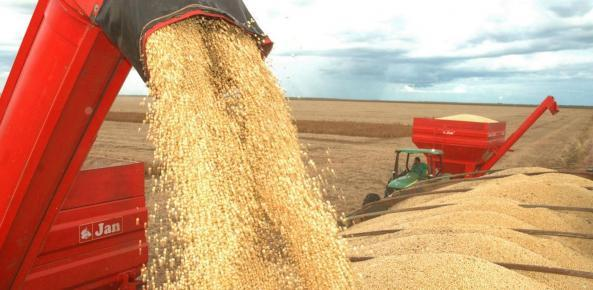
\includegraphics[width=0.6\textwidth]{images/grains_transport.jpg}
% 	\end{center}
% 	% {\centerline{\includegraphics[scale=#2]{#1}}}
% 	\vspace{-0.2cm}
% 	\label{fig:grains_transport}
% 	\legend{Fonte: Confederação da Agricultura e Pecuária do Brasil.\footnote{Disponível em: \url{http://www.cnabrasil.org.br/noticias/pesquisa-vai-quantificar-perdas-no-transporte-de-graos-em-caminhoes}. Acesso em: 04/11/2017}}
% 	% \vspace{-1cm}
% \end{figure}

Sendo assim, surge a necessidade de se compreender a mecânica das partículas.

A análise de sistemas de partículas, contudo, costuma ser bastante complexa. Partículas podem interagir umas com as outras e com o meio em que estão imersas. As interações podem ser forças de contato, forças de corpo, trocas de calor, trocas de carga elétrica, entre outras. Ainda, a quantidade de partículas presentes no sistema de interesse pode facilmente alcançar a ordem dos milhões \cite{bib:computational_granular_dynamics}. Além dessas dificuldades, os problemas estudados geralmente assumem geometrias distintas, tais quais a mistura de substâncias para a produção de fármacos ou o transporte de carga granular.

Com o propósito de executar tais análises, existem três abordagens principais: a experimental, a analítica e a numérica. 

No método experimental, procura-se caracterizar os fenômenos físicos através da sua reprodução em ambientes controlados. A grande vantagem desse método é o fato de lidar com a configuração real do sistema estudado, e dessa análise resultam hipóteses, equações e correlações para as diversas grandezas físicas envolvidas. A experimentação, no entanto, resulta em altíssimo custo e muitas vezes é limitada por questões de segurança ou pela dificuldade de reprodução do sistema real. A experimentação é utilizada para validar modelos físicos e matemáticos \cite{bib:maliska}.

A abordagem analítica, por sua vez, busca a obtenção de soluções analíticas para o problema. A vantagem de se obterem soluções em forma fechada é seu baixíssimo custo de computação quando comparado aos outros métodos. O método analítico, porém, frequentemente depende de hipóteses simplificativas e de geometrias e condições de contorno simples, o que acaba por reduzir a aplicabilidade de seus resultados. Geralmente, utilizam-se soluções analíticas para validar métodos numéricos e auxiliar na busca de métodos mais robustos \cite{bib:maliska}.

A fim de conciliar exatidão e eficiência, os métodos numéricos despontam como uma poderosa ferramenta capaz de resolver problemas complexos, com geometrias complicadas e grande número de partículas, alcançando, apesar disso, uma elevada rapidez e baixíssimo custo \cite{bib:maliska}.

\begin{figure}[h]
	\caption{Comparação entre experimento e simulação de pílulas no interior de um misturador.}
	\vspace{-0.5cm}
	\begin{center}
		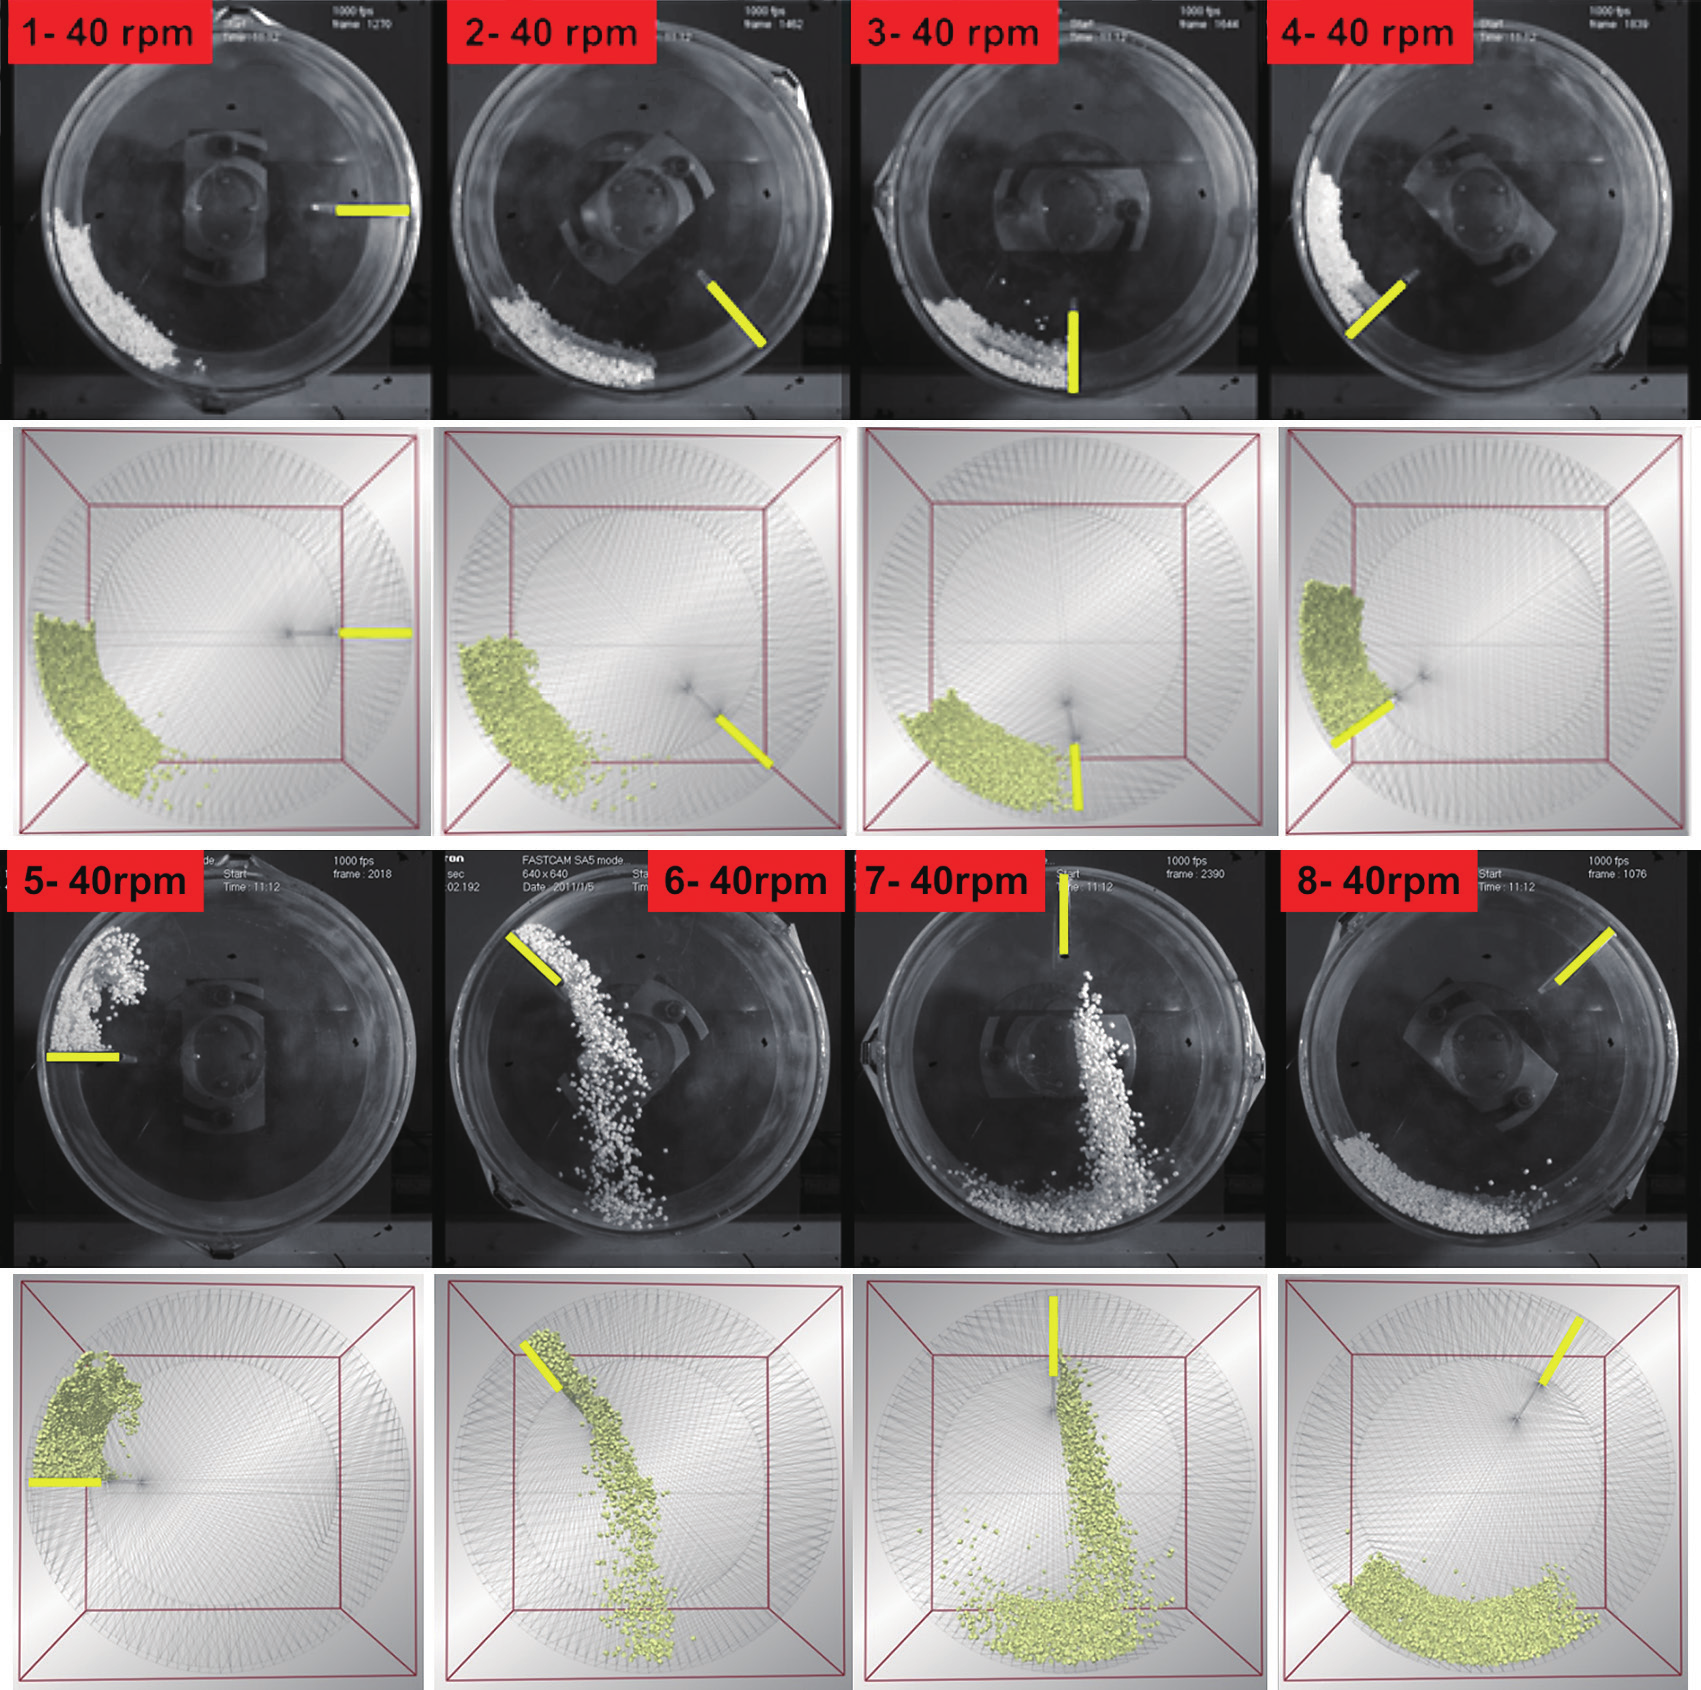
\includegraphics[width=0.65\textwidth]{images/pellet_flow.png}
	\end{center}
	% {\centerline{\includegraphics[scale=#2]{#1}}}
	\vspace{-0.2cm}
	\label{fig:pellet_flow}
	\legend{Fonte: \citeonline{bib:applications}.}
	% \vspace{-1cm}
\end{figure}

\begin{figure}[h]
	\caption{Comparação entre experimento e simulação da mistura de esferas de vidro no interior de um misturador.}
	\vspace{-0.5cm}
	\begin{center}
		\includegraphics[width=0.65\textwidth]{images/drug_production.png}
	\end{center}
	% {\centerline{\includegraphics[scale=#2]{#1}}}
	\vspace{-0.2cm}
	\label{fig:drug_production}
	\legend{Fonte: \citeonline{bib:future}.}
	\vspace{-1cm}
\end{figure}

As figuras \ref{fig:pellet_flow} e \ref{fig:drug_production} ilustram a capacidade dos métodos numéricos. A primeira delas é uma comparação feita por \citeonline{bib:applications} entre pílulas movendo-se no interior de um tambor rotativo experimentalmente e em uma simulação. A segunda figura representa uma comparação feita por \citeonline{bib:future} entre a mistura de esferas de vidro em um misturador e uma simulação correspondente. As esferas são idênticas a menos de sua cor, que permite uma melhor avaliação dos resultados. Como pode ser observado, embora as simulações não reproduzam \textit{exatamente} a posição das partículas, elas representam com grande fidelidade o sistema estudado.

Sendo assim, o estudo de sistemas de partículas conta principalmente com a simulação numérica como método de análise.
 
\section{Sistemas de Partículas}

A definição de partícula não é um consenso entre autores, cada um adotando o conceito mais adequado à aplicação. Segundo \citeonline{bib:sampaio}, compreende-se por \textit{partícula} um objeto ao qual são atribuídas propriedades físicas, mas cuja estrutura interna é desconsiderada. Cada partícula possui também uma função posição, que descreve a posição de seu centro de massa em função do tempo, e uma função orientação, que determina a posição dos seus eixos principais, sendo que essas duas definições são tomadas com relação a um sistema de referência fixo no espaço.

Por sua vez, um \textit{sistema de partículas} é um conjunto de partículas que interagem entre si. Conforme citado na \autoref{sec:motivation}, essas interações podem ser de diversas naturezas, das quais destacam-se as forças de colisão.

O aspecto dinâmico dos sistemas de partículas é determinado pelas leis de Euler para o movimento:
\begin{gather}
	{\resultingForce} = \mass\cdot\acceleration, \label{eq:intro_motion_first}\\
	{\resultingTorque} = \tensorOfInertia\cdot\deriv{1}{\angularVelocity} + \angularVelocity\cross\pqty{\tensorOfInertia\cdot\angularVelocity}, \label{eq:intro_motion_second}
\end{gather}
em que \(\position\), \(\angularVelocity\), \(\mass\) e \(\tensorOfInertia\) são, respectivamente, a função posição, a função velocidade angular, a massa e o tensor momento de inércia de uma partícula qualquer, enquanto \({\resultingForce}\) e \({\resultingTorque}\) são o vetor força resultante e o vetor torque resultante sobre a mesma.

É na solução das equações \eqref{eq:intro_motion_first} e \eqref{eq:intro_motion_second} que consiste a análise acerca dos sistemas de partículas. Essas equações, porém, são de difícil resolução já que a força e o torque resultantes sobre a partícula são oriundos de sua interação com os demais elementos do sistema e são, portanto, funções das propriedades físicas, posições, velocidades, orientações e velocidades angulares dos interagentes.

Em vista disso, é necessário o uso de métodos para a resolução dessas equações, e nessa situação destaca-se o Método dos Elementos Discretos.

\section{O Método dos Elementos Discretos} 

Segundo \citeonline{bib:sampaio}, o Método dos Elementos Discretos, ou DEM (\textit{Discrete Element Method}), refere-se a uma família de métodos computacionais que consideram deslocamentos e rotações de corpos discretos e reconhecem contatos entre elementos automaticamente à medida em que os cálculos são executados. Devido a essa característica, o DEM representa um conjunto de técnicas apropriadas para a simulação do comportamento dinâmico de sistemas de partículas.

De acordo com \citeonline{bib:cundall1979}, os cálculos são executados explicitamente, alternando entre a aplicação das leis de Euler para a determinação da posição e da orientação das partículas e a aplicação de relações força-deslocamento para a computação das forças e torques atuantes.

Geralmente, algoritmos de elementos discretos levam em conta a hipótese de partículas rígidas. Uma consequência disso é que, se uma partícula está em contato com outras duas, as interações ocorrem de maneira independente. Com isso, os contatos podem ser computados para cada par de partículas interagentes como se estivessem isoladas das demais.

Cada elemento da simulação pertence a um \textit{tipo}. O tipo de um elemento é usado para determinar a sua geometria e o seu comportamento na simulação. É comum, por exemplo, definir-se um tipo de partícula \textit{fixa}. Partículas desse tipo representam elementos de fronteira, com posição constante e conhecida desde o início da simulação.  

Por sua vez, a geometria das partículas determina quais os modelos de interação que podem ser aplicados. Em geral, o uso de geometrias simples permite a aplicação de modelos também simples, resultando em um custo computacional menor quando comparado às geometrias mais complexas. Certamente, a geometria de partícula necessária depende do sistema que se deseja estudar e do grau de representatividade requisitado. A geometria mais simples é a esférica. Para a obtenção de formas mais complexas, \citeonline{bib:computational_granular_dynamics} apresentam uma técnica de associação de partículas, resultando em partículas compostas, como aquela representada na figura \ref{fig:composite_particle}. \citeonline{bib:computational_granular_dynamics} também tratam de partículas poligonais, enquanto \citeonline{bib:sampaio} demonstra a utilização de superelipsoides.

\begin{figure}[h]
	\caption{Exemplo de associação de partículas simples para a obtenção de geometrias mais complexas.}
	% \vspace{-0.5cm}
	\begin{center}
		\alert{Colocar imagem de uma partícula composta}
		% \includegraphics[width=0.65\textwidth]{images/drug_production.png}
	\end{center}
	% {\centerline{\includegraphics[scale=#2]{#1}}}
	% \vspace{-0.2cm}
	\label{fig:composite_particle}
	\legend{Fonte: \alert{Citar fonte}}
	% \vspace{-1cm}
\end{figure}

O Método de Elementos Discretos é intimamente ligado à Dinâmica Molecular, outra família de métodos computacionais. A distinção que geralmente se faz é que o DEM considera geometrias arbitrariamente complexas, exigindo um tratamento da identificação dos pontos de contato e do cálculo das rotações mais adequado.

Segundo \citeonline{bib:computational_granular_dynamics}, algoritmos do DEM, de forma simplificada, são compostos por algumas etapas principais, sendo elas:
\begin{enumerate}
	\item \textbf{Inicialização:} Nesta etapa, os elementos da simulação são construídos, cada qual com tipo, geometria, propriedades físicas, posição e velocidade iniciais. Também são determinados os modelos de interação considerados e o critério de parada. Esses itens são geralmente definidos por um arquivo de entrada.
	\item \textbf{Predição:} O cálculo de forças e torques atuantes sobre cada partícula depende da posição, da velocidade, da orientação e da velocidade angular dos elementos da simulação, que são desconhecidas no instante futuro. Sendo assim, é necessária uma estimativa, ou \textit{predição}, para os valores dessas variáveis. Essa estimativa é feita na etapa de predição. \label{item:prediction}
	\item \textbf{Interação:} A etapa de interação se divide em duas subetapas:
		\begin{enumerate}
			\item Determinação dos pares de interação. Nem todas as partículas interagem em todos os instantes.
			\item Computação das forças e torques entre os elementos da simulação com base nas coordenadas previstas na etapa \ref{item:prediction}.
		\end{enumerate}
	\item \textbf{Correção:} Nesta etapa, valores corrigidos para as coordenadas (e as respectivas derivadas) das partículas são obtidos através da resolução das equações \eqref{eq:intro_motion_first} e \eqref{eq:intro_motion_second}.
	\item \textbf{Terminação:} Caso o critério de parada previamente estabelecido seja atingido, o programa deve finalizar. Caso contrário, a simulação deve avançar o instante de tempo e retornar ao passo \ref{item:prediction}.
\end{enumerate}

Essas etapas podem ser representadas como na figura \ref{fig:simple_dem_algorithm}. Outros passos podem ser introduzidos no algoritmo, tais quais exportação de dados, iterações em cada passo de tempo e acoplamento com outros simuladores.

\begin{figure}[h]
	\caption{Fluxograma simplificado do Método dos Elementos Discretos.}
	% \vspace{-0.5cm}
	\begin{center}
		\alert{Colocar fluxograma do DEM}
		% \includegraphics[width=0.65\textwidth]{images/drug_production.png}
	\end{center}
	% {\centerline{\includegraphics[scale=#2]{#1}}}
	% \vspace{-0.2cm}
	\label{fig:simple_dem_algorithm}
	\legend{Fonte: \alert{Citar fonte}}
	% \vspace{-1cm}
\end{figure}

Também é possível acoplar o DEM a outras famílias de métodos, como FEM (Método de Elementos Finitos) e CFD (Fluidodinâmica Computacional). Nesses casos, além das equações de movimento para as partículas, são consideradas equações de conservação de massa, de energia, de carga elétrica, equações de estado, entre outras. Com isso, é possível computar transferência de calor, arraste causado por fluidos e distribuição de tensões em sólidos. \citeonline{bib:donze} e \citeonline{bib:dem_chapter} apresentam alguns exemplos das diversas extensões que podem ser feitas ao DEM. \citeonline{bib:chu_and_yu} explicam e aplicam um modelo para interação entre um fluido e partículas com foco no arrasto, enquanto \citeonline{bib:conductivity} e \citeonline{bib:heat_dem} demonstram a aplicação de modelos de troca de calor. O acoplamento entre DEM e outras famílias é conhecido como EDEM, ou XDEM, o Método de Elementos Discretos Estendido.

\section{Revisão Bibliográfica}

A base matemática para os Métodos de Elementos Discretos foi fundada por Isaac Newton, com a divulgação de suas leis de movimento. Entretanto, devido às dificuldades mencionadas na seção \ref{sec:motivation} tais quais a quantidade de partículas e a natureza das equações diferenciais, a análise de sistemas de partículas só se tornou factível com o advento dos computadores.

O Método dos Elementos Discretos foi primeiramente apresentado por Cundall. Uma descrição do método pode ser encontrada em \citeonline{bib:cundall1979}, em que se consideram atrito e amortecimento na colisão das partículas. A presença de atrito provoca rotações, que devem ser solucionadas juntamente com as posições. Nesse algoritmo, as velocidades eram preditas como constantes durante um passo de tempo.

O método foi ainda extendido com os trabalhos de \citeonline{bib:haff1986}, \apudonline{bib:walton1983}{bib:haff1986}, \citeonline{bib:gallas1992}, além de vários outros.

Dentre as principais referências sobre o DEM, destacam-se \citeonline{bib:liquids}, \citeonline{bib:computational_granular_dynamics} e \citeonline{bib:dem_chapter}.

Além das publicações acadêmicas, existem diversos \textit{softwares} comerciais e de código aberto projetados para simulação com o DEM, cada qual com seus objetivos, vantagens e desvantagens. Dentre os simuladores comerciais, destacam-se o Rocky DEM, o EDEM e o PFD (\textit{Particle Flow Code}). Dentre os principais programas de código aberto estão o Yade, o LIGGGHTS e o KRATOS. Algumas das características desses simuladores são o processamento em paralelo, a capacidade de customização, pós-processamento, geração de scripts, acoplamento entre diferentes físicas, uso de geometrias CAD e acoplamento com outros simuladores.

\section{Objetivos e Contribuições}

O SINMEC - Laboratório de Simulação Numérica em Mecânica dos Fluidos e Transferência de Calor, do Departamento de Engenharia Mecânica da Universidade Federal de Santa Catarina, tem como principal linha de pesquisa a aplicação do método de volumes finitos baseado em elementos (EbFVM) com malhas não estruturadas para a solução de problemas de mecânica de fluidos e transferência de calor.

Devido à importância do tema e à possibilidade de se estudar o acoplamento entre a dinâmica de partículas e os fenômenos de transporte, surgiu o interesse do laboratório em iniciar uma área de pesquisa acerca do Método de Elementos Discretos Estendido utilizando o EbFVM para a solução de escoamentos. Para tanto, porém, é necessária, primeiramente, uma compreensão acerca do DEM.

Sendo assim, este trabalho objetiva iniciar essa linha de pesquisa no SINMEC, desenvolvendo um simulador que seja de fácil extensão, permitindo que novos modelos de interação, tipos de partículas e algoritmos de solução sejam introduzidos à medida que novos estudos sejam feitos. Para que isso se tornasse possível, este trabalho foi subdividido em três partes: primeiramente, uma biblioteca deveria ser implementada, contendo a lógica do funcionamento dos algoritmos DEM, de forma generalizada, sem particularizar suas características; na segunda parte, seria gerado um simulador que, tomando a biblioteca como base, especificasse os tipos de partícula, as interações e os métodos de solução; e, por fim, executar simulações no simulador e validar a implementação através da análise dos resultados e da comparação com soluções analíticas. 
 
Com o propósito de melhor guiar as atividades, são propostos os seguintes objetivos específicos:
\begin{enumerate}
\item Desenvolver uma biblioteca computacional para a simulação da dinâmica de partículas através do DEM. Essa biblioteca deve possuir as seguintes características: \label{item:library}
 	\begin{enumerate}
		\item Suporte para diferentes modelos de colisão, inclusive para modelos estudados e implementados por um usuário posterior;
		\item Capacidade para um número arbitrário de partículas, as quais podem assumir diferentes formas geométricas e possuir várias propriedades físicas;
        \item Permitir a inserção de diferentes tipos de interação entre as partículas. Essas interações podem ter naturezas distintas, como a transferência de calor e a troca de cargas elétricas;
		\item Suporte para variadas funções de busca de partículas vizinhas;
		\item Disponibilidade de utilização de diversos tipos de condição de contorno;
		\item Suporte para diferentes algoritmos de predição e correção;
	\end{enumerate}  
\item Implementar um simulador que, com base na biblioteca desenvolvida, seja capaz de executar simulações que aceitem, no mínimo:
	\begin{enumerate}
		\item Partículas esféricas;
		\item Paredes fixas planas;
		\item Os principais modelos de força de colisão, conforme explicado na seção \ref{sec:collision_force_models};
		\item O algoritmo de Gear, empregando a extrapolação de Taylor, de acordo com o capítulo \ref{ch:mathematical_model};
		\item Três dimensões;
	\end{enumerate}
\item Validar a implementação por meio da comparação de resultados de simulações com soluções analíticas para o problema ou através da análise dos resultados.
\end{enumerate}

\section{Organização do Trabalho}

Para melhor cobrir todos os assuntos relativos ao cumprimento dos objetivos, além do capítulo de introdução, este trabalho é dividido nos seguintes capítulos:
\begin{description}
	\item[\autoref{ch:mathematical_model} - \nameref{ch:mathematical_model}:] Nesse capítulo, são abordados os aspectos teóricos e matemáticos concernentes ao DEM. Nele, são descritas as equações de movimento que devem ser solucionadas, alguns dos principais modelos para as forças de colisão e o algoritmo de Gear;
	\item[\autoref{ch:discrete_element_method} - \nameref{ch:discrete_element_method}:] Nesse capítulo, é descrito o DEM, demonstrando como os conceitos apresentados no capítulo \ref{ch:mathematical_model} são aplicados e transformados em algoritmos.
	\item[\autoref{ch:computational_implementation} - \nameref{ch:computational_implementation}:] Esse capítulo evidencia a implementação da biblioteca e do simulador em linguagem C++ ao apresentar códigos, pseudocódigos e fluxogramas com o intuito de fornecer uma visão geral do código e explicar o seu funcionamento.
	\item[\autoref{ch:results} - \nameref{ch:results}:] Esse capítulo é destinado à apresentação de resultados de simulação, à sua confrontação com soluções analíticas e à análise de tais resultados. Com isso, a implementação é validada.
	\item[\autoref{ch:conclusion} - \nameref{ch:conclusion}:] O último capítulo é dedicado a sumarizar o trabalho, reafirmando os principais pontos explorados ao longo do texto e atestando que os objetivos propostos foram alcançados. Também são apresentadas algumas sugestões para trabalhos futuros.
\end{description}

\chapter{Modelo Matemático} \label{ch:mathematical_model}

Segundo \citeonline{bib:maliska}, a solução numérica de qualquer problema físico requer a sua prévia modelagem matemática. Um modelo matemático é uma representação de um sistema real através de equações. Essas equações são obtidas ao se fazerem hipóteses sobre o comportamento do sistema estudado, e a representatividade do modelo depende das simplificações feitas nesse processo.

Este capítulo aborda os aspectos matemáticos pertinentes ao Método de Elementos Discretos. São abordados os principais conceitos referentes aos sistemas de partículas, e apresentadas as equações de movimento que governam o problema. Os principais modelos de força de colisão são então expostos e, por fim, é apresentado o algoritmo de Gear, responsável por resolver as equações.

\section{Sistemas de Partículas} \label{sec:particle_systems}

As partículas são os elementos fundamentais do Método de Elementos Discretos. De acordo com a definição apresentada por \citeonline{bib:sampaio}, partículas são consideradas corpos rígidos. Por serem indeformáveis, fica implícita a hipótese de que não ocorrem deformações plásticas nesses elementos, e então eles preservam a sua geometria mesmo durante e após colisões.

A princípio, o \DEM{} suporta geometrias arbitrárias para seus elementos. Entretanto, devido a limitações de modelos físicos e de avaliação das colisões, em geral consideram-se formatos básicos como esferas, superelipsoides e poliedros. Geometrias mais complexas podem ser geradas pela associação de geometrias mais simples em partículas compostas \cite{bib:sampaio,bib:computational_granular_dynamics}.

Um sistema de partículas é, por sua vez, um conjunto de partículas que interagem entre si. Considera-se que o sistema possua um referencial global fixo centrado no ponto \(\originPoint\) a partir do qual as demais grandezas vetoriais são definidas.

A cada partícula está associada uma função posição que determina, vetorialmente, a posição de seu centro de massa com relação à origem do sistema. A orientação de um elemento é a orientação do seu sistema de eixos principais com relação ao sistema global. Com isso, cada partícula possui seis graus de liberdade: três translações e três rotações \cite{bib:sampaio}. Os elementos discretos ainda contêm diversas \textit{propriedades}, as quais são determinantes para as suas interações.

As translações e rotações das partículas são determinadas através da solução das equações de movimento, detalhadas na seção \ref{sec:equations_of_motion}. Essas equações dependem das interações que ocorrem entre as partículas. Em um sistema qualquer, as interações podem ser de diversas naturezas, tais quais colisões mecânicas, troca de cargas elétricas, transferência de calor, e outras. No entanto o \DEM{} considera, a princípio, apenas as colisões e as forças de campo, como a gravidade.

Embora a quantidade de elementos em um sistema seja arbitrária, ela é sempre finita. Denotando por \(\numberOfParticles\) essa quantidade, é possível enumerarem-se esses elementos e definir-se o conjunto de partículas do sistema como
\begin{equation*}
	\particleSet = \left\lbrace\particlei \suchThat 1\leq i\leq\numberOfParticles\right\rbrace,
\end{equation*}
sendo \(\particlei\) a \(i\)-ésima partícula no sistema.

Cada partícula ainda possui uma \textit{vizinhança}, que é o conjunto de elementos que podem interagir com ela. Denota-se por \(\ineighborhood{i}\) ou \(\neighborhoodOf{\particlei}\) a vizinhança da partícula \(i\). A determinação da vizinhança de uma partícula é essencial para o cálculo das forças e dos torques que atuam sobre ela, e alguns dos métodos para se construir esse conjunto são apresentados na \autoref{sec:neighborhood}.

Escrevendo como \(\forceji\) a força e \(\torqueji\) o torque aplicados pela partícula \(\particlej\) sobre a partícula \(\particlei\), tem-se que a força resultante \(\resultingForcei\) e o torque resultante \(\resultingTorquei\) sobre \(\particlei\) são dados pelo princípio da superposição como
\begin{gather}
	\resultingForcei = \sum_{\particlej\in\ineighborhood{i}}\forceji + \external\resultingForcei, \label{eq:superposition_translation} \\
	\resultingTorquei = \sum_{\particlej\in\ineighborhood{i}}\torqueji + \external\resultingTorquei, \label{eq:superposition_rotation}
\end{gather}
em que \(\external\resultingForcei\) e \(\external\resultingTorquei\) são a força e o torque \textit{externos} atuantes sobre \(\particlei\), isto é, resultantes da interação entre a \(i\)-ésima partícula com elementos exteriores ao sistema.

Uma importante hipótese que se faz no Método de Elementos Discretos é que a interação entre duas partículas \(\particlei\) e \(\particlej\) não interfere na interação entre outras partículas ou entre \(\particlei\) e uma terceira partícula \(\particlek\). Com isso, cada par de partículas pode ser estudado isoladamente, e o estado final do sistema, após as interações, é uma simples combinação desses resultados.

\section{Equações de Movimento} \label{sec:equations_of_motion}

Na dinâmica de partículas, os elementos estudados são considerados corpos rígidos, aos quais se aplicam as leis de Euler para o movimento \cite{bib:sampaio, bib:dynamics_of_multibody_systems}.

Em um sistema inercial fixo, considera-se uma partícula de massa \(\mass\) com um centro de massa \(C\) cuja posição é descrita pela função vetorial \(\position\). Além disso, considera-se que a partícula possua uma velocidade angular \(\angularVelocity\) e um tensor momento de inércia \(\tensorOfInertia\) definido com relação ao seu centro de massa.

Conforme demonstrado por \citeonline{bib:dynamics_of_multibody_systems}, a \textit{quantidade de movimento linear} e a \textit{quantidade de movimento angular} da partícula, denotadas respectivamente por \(\linearMomentum\) e \(\angularMomentum\), são então dadas por
\begin{gather*}
	\linearMomentum = \mass\cdot\velocity, \\
	\angularMomentum = \position\cross\linearMomentum + \tensorOfInertia\cdot\angularVelocity.
\end{gather*}

\subsection{Primeira Lei de Euler}

A primeira lei de Euler trata do movimento de translação. Ela se expressa através da equação
\begin{equation} \label{eq:euler_first}
	\resultingForce = \deriv{1}{\linearMomentum},
\end{equation}
sendo \(\resultingForce\) o vetor força resultante sobre a partícula. Para o caso em que a massa do corpo é constante, a primeira lei de Euler torna-se equivalente à segunda lei de Newton:
\begin{equation} \label{eq:motion_first}
	\resultingForce = \mass\cdot\acceleration.
\end{equation}

A equação \eqref{eq:euler_first} é aplicada para os fenômenos de fragmentação e aglutinação, casos em que partículas são divididas ou unidas, sendo que a massa de cada partícula isoladamente não é constante. \citeonline{bib:computational_granular_dynamics} apresentam métodos que descrevem o fenômeno de fragmentação. Tais situações, porém, são tratadas separadamente, de modo que a equação \eqref{eq:motion_first} é a que se considera para o estudo da evolução do sistema.

De acordo com o princípio da superposição, a força resultante sobre a partícula é igual à soma vetorial todas as forças aplicadas sobre ela, conforme a equação \eqref{eq:superposition_translation}. Essas forças são comumente divididas em \textit{forças internas} e \textit{forças externas} ao sistema. As forças internas são aquelas oriundas das interações entre os elementos do sistema, enquanto as forças externas são atribuídas a elementos exteriores. 

No sistema, as forças internas são sempre sujeitas ao princípio de ação e reação. Se a partícula \(\particlei\) aplica uma força \(\forceij\) sobre a partícula \(\particlej\), então, pela terceira lei de Newton,  a força \(\forceji\) que \(\particlej\) aplica sobre \(\particlei\) é dada por
\begin{equation*}
	\forceji = - \forceij.
\end{equation*}

Para a translação, os movimentos ocorrem separadamente em cada eixo coordenado de modo que os algoritmos de solução da equação \eqref{eq:motion_first} são facilmente generalizados de duas para três dimensões. Ainda, cabe observar que a primeira lei de Euler independe da posição do eixo de referência. Isso nem sempre ocorre no movimento de rotação.

\subsection{Segunda Lei de Euler}

A segunda lei de Euler, por sua vez, é o análogo rotacional da primeira:
\begin{equation*} % \label{eq:euler_second}
	\resultingTorque = \deriv{1}{\angularMomentum},
\end{equation*}
em que \(\resultingTorque\) é o torque resultante sobre a partícula calculado com relação ao seu centro de massa. Para partículas com massa constante, é possível obter
\begin{equation} \label{eq:motion_second}
	\resultingTorque = \deriv{1}{\angularMomentum} = \tensorOfInertia\cdot\deriv{1}{\angularVelocity} + \angularVelocity\cross\pqty{\tensorOfInertia\cdot\angularVelocity},
\end{equation}
sendo \(\angularVelocity\) a \textit{aceleração angular} do elemento.

Novamente, a hipótese de que a massa da partícula é constante é geralmente considerada. 

Entretanto, mesmo diante de situações em que \(m\) é constante, a resolução da equação \eqref{eq:motion_second} possui algumas complicações em simulações tridimensionais. Isso se deve ao fato de que são necessárias parametrizações para a orientação da partícula, e não ocorre que a velocidade angular seja a derivada desses parâmetros. Só é possível escrever \(\angularVelocity = \deriv{1}{\orientation}\), isto é, a velocidade angular como taxa de variação de uma função de orientação, quando a direção da rotação é constante \cite[p. 32]{bib:dynamics_of_multibody_systems}.

O tensor \(\tensorOfInertia\) identifica-se com a matriz de momento de inércia \(\matrixOfInertia\) dada por
\begin{equation*}
	\matrixOfInertia =
	\begin{pmatrix}
		\xxMomentOfInertia & \xyMomentOfInertia & \xzMomentOfInertia \\
		\yxMomentOfInertia & \yyMomentOfInertia & \yzMomentOfInertia \\
		\zxMomentOfInertia & \zyMomentOfInertia & \zzMomentOfInertia
	\end{pmatrix}.
\end{equation*}

Para um ponto \(P\) qualquer, define-se o vetor radial \(\radialVector = \vectorFromPoints{C}{P}\). Denotando por \(\radialVectorMtx\) a matriz correspondente a \(\radialVector\), a matriz de momento de inércia do corpo \(\particlei\) é dada por
\begin{equation*}
	\matrixOfInertia = \int_{\particlei}\pqty{\transpose{\radialVectorMtx}\radialVectorMtx\cdot\identity - \radialVectorMtx\transpose{\radialVectorMtx}}\dd{m},
\end{equation*}
em que \(\identity\) é a matriz identidade. Alternativamente, escrevendo-se \(\radialVector = \explicitVectorCoordinates{\radialVectorScalar}\),
\begin{equation*}
	\matrixOfInertia =
	\begin{pmatrix}
		\dint_{\particlei} \pqty{\yComponent{\radialVectorScalar}^2 + \zComponent{\radialVectorScalar}^2} \dd{m}
		& - \dint_{\particlei} \xComponent{\radialVectorScalar}\yComponent{\radialVectorScalar} \dd{m}
		& - \dint_{\particlei} \xComponent{\radialVectorScalar}\zComponent{\radialVectorScalar} \dd{m} \\
		& \dint_{\particlei} \pqty{\xComponent{\radialVectorScalar}^2 + \zComponent{\radialVectorScalar}^2} \dd{m} 
		& - \dint_{\particlei} \yComponent{\radialVectorScalar}\zComponent{\radialVectorScalar} \dd{m} \\
		\text{Simétrica} 
		&  
		& \dint_{\particlei} \pqty{\xComponent{\radialVectorScalar}^2 + \yComponent{\radialVectorScalar}^2} \dd{m}
	\end{pmatrix}.
\end{equation*}

A cada corpo estão associados \textit{eixos principais}, formados pelos autovetores da matriz de momento de inércia. Ao se utilizarem como sistema de referência os eixos principais, a matriz de inércia assume forma diagonal:
\begin{equation*}
	\principal{\matrixOfInertia} =
	\begin{pmatrix}
		\momentOfInertia_1 & 0 & 0 \\
		0 & \momentOfInertia_2 & 0 \\
		0 & 0 & \momentOfInertia_3 \\
	\end{pmatrix},
\end{equation*}
e reescrevendo, nessas coordenadas, o torque resultante como \(\principal{\resultingTorque} = \explicitVectorPrincipalCoordinates{\torqueScalar}\), a velocidade angular como \(\principal{\angularVelocity} = \explicitVectorPrincipalCoordinates{\angularVelocityScalar}\) e a aceleração angular como \(\principal{\angularAcceleration} = \explicitVectorPrincipalCoordinates{\deriv{1}{\angularVelocityScalar}}\), a equação \eqref{eq:motion_second} se transforma no sistema de equações
\begin{equation} \label{eq:motion_second_system}
	\left\lbrace
	\begin{array}{l}
		\momentOfInertia_1\deriv{1}{\angularVelocityScalar}_1 - \pqty{\momentOfInertia_2 - \momentOfInertia_3}\angularVelocityScalar_2\angularVelocityScalar_3 = \torqueScalar_1 \\
		\momentOfInertia_2\deriv{1}{\angularVelocityScalar}_2 - \pqty{\momentOfInertia_3 - \momentOfInertia_1}\angularVelocityScalar_3\angularVelocityScalar_1 = \torqueScalar_2 \\
		\momentOfInertia_3\deriv{1}{\angularVelocityScalar}_3 - \pqty{\momentOfInertia_1 - \momentOfInertia_2}\angularVelocityScalar_1\angularVelocityScalar_2 = \torqueScalar_3
	\end{array}
	\right.
	.
\end{equation}

Esse sistema pode ser resolvido de forma análoga à primeira lei de Euler, conforme discutido na \autoref{subsec:motion_equations_solution}. Os valores de \(\momentOfInertia_1\), \(\momentOfInertia_2\) e \(\momentOfInertia_3\) são dependentes da geometria da partícula e da distribuição de massa no seu interior. Em geral, essas características já são conhecidas no início das simulações.

Entretanto o sistema \eqref{eq:motion_second_system} exige que se conheçam os eixos principais da partícula, isto é, sua orientação. Esses eixos, porém, movem-se e rotacionam junto com o corpo, e então são variantes no tempo. Para se resolver o problema no caso geral, são propostas parametrizações, tais quais os ângulos de Euler, os ângulos de Bryan, e os parâmetros de Euler-Rodrigues \cite{bib:dynamics_of_multibody_systems}. Mais detalhes sobre essas parametrizações são encontrados no \autoref{app:three_dimensional_rotation}.

\alert{Verificar que os detalhes foram explicados no apêndice}

Duas simplificações que podem se aplicar à equação \eqref{eq:motion_second} são: que a simulação ocorre em apenas duas dimensões; ou que as partículas são esféricas. No primeiro caso, a direção de rotação é constante. Essa situação é tratada na \autoref{subsubsec:bidimensional}. Já no segundo caso, como explicado na \autoref{subsubsec:rotation_of_spherical_particles}, qualquer sistema de eixos centrado no centro de massa da partícula é um sistema de eixos principais, e então a orientação das partículas não é mais necessária para a determinação de \eqref{eq:motion_second_system}. Por fim, na \autoref{subsubsec:general_rotation}, apresenta-se o caso de rotação geral em três dimensões.

\subsubsection{Simulação Bidimensional} \label{subsubsec:bidimensional}

Em se supondo que a simulação ocorre em apenas duas dimensões, por convenção no plano \(\xAxis\yAxis\), a velocidade angular das partículas possui direção constante, a do eixo \(\zAxis\). Denotando por \(\basis = \pqty{\xUnit, \yUnit, \zUnit}\) a base canônica do espaço \(\real^3\), isso implica que existe uma função real \(\angularVelocityScalar\) tal que
\[
	\angularVelocity = \angularVelocityScalar\cdot\zUnit.
\]

Já que, neste caso, a velocidade angular possui direção constante, é possível encontrar uma função \(\orientationScalar\) para a orientação da partícula, de forma que
\begin{gather*}
	\angularVelocityScalar = \deriv{1}{\orientationScalar}, \\
	\angularVelocity = \deriv{1}{\orientationScalar}\cdot\zUnit, \text{e} \\
	\angularAcceleration = \deriv{2}{\orientationScalar}\cdot\zUnit.
\end{gather*}

Geometricamente, \(\orientationScalar\) é o ângulo entre os eixos principais da partícula e sua orientação de referência, como na figura \ref{fig:bidimensional_simulation}.

\begin{figure}[h]
	\caption{Ângulo de rotação de uma partícula com relação à posição de referência em simulações bidimensionais}
	% \vspace{-0.5cm}
	\centering
		\alert{Colocar imagem representando a orientação de uma partícula em simulação bidimensionais}
		% \includegraphics[width=0.65\textwidth]{images/drug_production.png}
	% {\centerline{\includegraphics[scale=#2]{#1}}}
	% \vspace{-0.2cm}
	\label{fig:bidimensional_simulation}
	\source{\alert{Citar fonte}}
	% \vspace{-1cm}
\end{figure}

Além disso, da hipótese de que as rotações ocorrem apenas em torno do eixo \(\zAxis\) segue que o torque resultante possui apenas componentes nessa direção, isto é,
\begin{equation*}
	\resultingTorque = \torqueScalar\cdot \zUnit,
\end{equation*}
com \(\torqueScalar\in\real\).

Com isso, a equação \eqref{eq:motion_second} fica simplesmente
\begin{equation*}
	\torqueScalar = \zzMomentOfInertia\cdot\deriv{2}{\orientationScalar},
\end{equation*}
em que \(\zzMomentOfInertia\) é o momento de inércia escalar da partícula com relação ao eixo \(\zAxis\). Essa última equação se torna, então, a equação de movimento rotacional para partículas em simulações em duas dimensões.

Uma situação um pouco mais geral é que a direção da velocidade angular seja apenas constante, não necessariamente a do eixo \(\zAxis\), mas sim a de um eixo qualquer \(\zAxis^\prime\). Nesse caso, existe uma nova base \(\basis^\prime = \explicitVector{\xUnit^\prime}{\yUnit^\prime}{\zUnit^\prime}\) contendo os versores dos eixos \(\xAxis^\prime\yAxis^\prime\zAxis^\prime\) que satisfaz
\begin{equation*}
	\angularVelocity = \angularVelocityScalar\cdot\zUnit^\prime,
\end{equation*}
e, analogamente ao caso anterior, uma função de orientação \(\orientationScalar\) tal que
\begin{gather*}
	\angularVelocity = \deriv{1}{\orientationScalar}\cdot\zUnit^\prime, \\
	\angularAcceleration = \deriv{2}{\orientationScalar}\cdot\zUnit^\prime.
\end{gather*}

Novamente, a hipótese de direção de rotação constante implica que é possível escrever
\begin{equation*}
	\resultingTorque = \torqueScalar\cdot\zUnit^\prime,
\end{equation*}
e assim se obtém a equação
\begin{equation*}
	\torqueScalar = \zzMomentOfInertia^\prime\cdot\deriv{2}{\orientationScalar}.
\end{equation*}

Para a solução dessa equação, porém, ainda é necessária a determinação do valor de \(\zzMomentOfInertia^\prime\). Isso pode ser feito como sugere \citeonline{bib:dynamics_of_multibody_systems}, calculando-se a matriz de rotação \(\rotationMatrix\) que transforma as coordenadas de vetores definidos na base \(\basis\) em coordenadas definidas no sistema \(\xAxis^\prime\yAxis^\prime\zAxis^\prime\), na base \(\basis^\prime\), e obtendo
\begin{equation*}
	\matrixOfInertia^\prime =
	\begin{pmatrix}
		\xxMomentOfInertia^\prime & \xyMomentOfInertia^\prime & \xzMomentOfInertia^\prime \\
		\yxMomentOfInertia^\prime & \yyMomentOfInertia^\prime & \yzMomentOfInertia^\prime \\
		\zxMomentOfInertia^\prime & \zyMomentOfInertia^\prime & \zzMomentOfInertia^\prime
	\end{pmatrix}
	=
	\rotationMatrix\cdot \matrixOfInertia \cdot \transpose{\rotationMatrix}.
\end{equation*}

Embora tenda-se a evitar multiplicações matriciais, esse cálculo pode ser feito apenas uma vez, no início da simulação, desde que se saiba a priori a direção da rotação.

\subsubsection{Rotação de Partículas Esféricas} \label{subsubsec:rotation_of_spherical_particles}

Segundo \citeonline{bib:dynamics_of_multibody_systems}, para partículas esféricas, \textit{todas} as direções são uma direções principais. Sendo assim, o sistema de equações \eqref{eq:motion_second_system} é válido em qualquer sistema de eixos. Mais ainda, em função da simetria da partícula, ocorre que \(\momentOfInertia_1 = \momentOfInertia_2 = \momentOfInertia_3\). Ao se definir \(\momentOfInertia \eqdef \momentOfInertia_1\), obtém-se
\begin{equation*}
	\left\lbrace
	\begin{array}{l}
		\momentOfInertia\deriv{1}{\angularVelocityScalar_1} = \torqueScalar_1 \\
		\momentOfInertia\deriv{1}{\angularVelocityScalar_2} = \torqueScalar_2 \\
		\momentOfInertia\deriv{1}{\angularVelocityScalar_3} = \torqueScalar_3
	\end{array}
	\right.
	,
\end{equation*}
ou ainda
\begin{equation} \label{eq:rotation_spherical_particle}
	\resultingTorque = \momentOfInertia\cdot\angularAcceleration,
\end{equation}
sendo que o momento de inércia \(\momentOfInertia\) é facilmente calculado pela expressão
\begin{equation} \label{eq:momentOfInertia_for_spheres}
	\momentOfInertia = \dfrac{2}{5}\cdot\mass \radius^2,
\end{equation}
em que \(\radius\) é o raio da esfera.

Com isso, a equação diferencial para o movimento de rotação está pronta para simulações tridimensionais de partículas esféricas.

\subsubsection{Rotação Geral em Três Dimensões} \label{subsubsec:general_rotation}

Para simulações em três dimensões com partículas não esféricas, utiliza-se o sistema de equações \eqref{eq:motion_second_system}. A solução do sistema, porém, não é trivial já que as equações são dadas em termos das direções principais da partícula.

As direções principais de uma partícula são dadas pela base ortonormal \(\principal{\basis} = \explicitVector{\principal{\xUnit}}{\principal{\yUnit}}{\principal{\zUnit}}\) cujos versores são autovetores da matriz de momento de inércia. A importância dessa base se dá pelo fato de que a matriz de momento de inércia se torna diagonal quando escrita em termos de seus vetores.

Entretanto, em virtude do caráter dinâmico dos sistemas de partículas, as direções principais dos elementos são funções do tempo: \(\principal{\basis} \equiv \principal{\basis}\pqty{t}\). Uma \textit{parametrização} para a orientação é qualquer conjunto de coordenadas \(\orientation\) que defina, equivalentemente, as direções principais. Diversas parametrizações já foram propostas, como mostrado no \autoref{app:three_dimensional_rotation}.

Com a parametrização \(\orientation\), sempre é possível obter os eixos principais através de uma transformação inversível:
\begin{equation*}
	\principal{\basis}\pqty{t} \leftrightarrow \orientation\pqty{t},
\end{equation*}
e, com isso, determina-se uma matriz de rotação \(\orientationRotationMatrix\) que transforma vetores da base de eixos locais na base das direções principais da partícula.

Ainda, com os eixos principais dados em função de \(\orientation\), a velocidade angular e suas derivadas podem ser escritas a partir da parametrização e suas derivadas:
\begin{gather*}
	\angularVelocity \equiv \angularVelocity\pqty{\orientation, \deriv{1}{\orientation}}, \\
	\deriv{1}{\angularVelocity} \equiv \deriv{1}{\angularVelocity}\pqty{\orientation, \deriv{1}{\orientation}, \deriv{2}{\orientation}}, \\
	\vdots \\
	\deriv{\taylorOrder}{\angularVelocity} \equiv \deriv{\taylorOrder}{\angularVelocity}\pqty{\orientation, \deriv{1}{\orientation}, \dots, \deriv{\taylorOrder+1}{\orientation}}.
\end{gather*}

Essas relações são inversíveis, e então é possível obter
\begin{gather*}
	\deriv{1}{\orientation} \equiv \deriv{1}{\orientation}\pqty{\orientation, \angularVelocity} \\
	\deriv{2}{\orientation} \equiv \deriv{2}{\orientation}\pqty{\orientation, \angularVelocity, \deriv{1}{\angularVelocity}} \\
	\vdots \\
	\deriv{\taylorOrder+1}{\orientation} \equiv \deriv{\taylorOrder+1}{\orientation}\pqty{\orientation, \angularVelocity, \dots, \deriv{\taylorOrder}{\angularVelocity}}
\end{gather*}

Assim, com a parametrização \(\orientation\), define-se toda a cinemática da rotação da partícula. Mais ainda, devido à equivalência entre o sistema de eixos principais e a parametrização, vetores definidos com relação ao sistema de eixos locais podem ser escritos em termos das direções principais. Isso significa que
\begin{equation*}
	\principal{\resultingTorque} \equiv \principal{\resultingTorque}\pqty{\resultingTorque, \orientation}.
\end{equation*}

Como resultado dessas considerações, o sistema de equações \eqref{eq:motion_second_system} transforma-se em uma equação diferencial da forma
\begin{equation} \label{eq:diff_equation_orientation_parametrization}
	\deriv{2}{\orientation} = \eqFor{\orientation}\pqty{\resultingTorque, \orientation, \deriv{1}{\orientation}}.
\end{equation}

A função \(\eqFor{\orientation}\) representa a dependência de \(\deriv{2}{\orientation}\) com relação a \(\resultingTorque\), \(\orientation\) e \(\deriv{1}{\orientation}\), e seu formato depende da definição da parametrização e da expressão para o torque resultante em função das variáveis do problema.

\subsection{Solução das Equações de Movimento} \label{subsec:motion_equations_solution}

Para a determinação do comportamento do sistema, é necessária a obtenção das soluções para as equações \eqref{eq:motion_first} e \eqref{eq:motion_second}. Isso exige  o cálculo da força e do torque resultantes sobre cada partícula e a consequente resolução da equação. 

O cálculo das forças e dos torques geralmente leva em conta \textit{modelos de interação}. Cada modelo determina uma parcela do vetor força ou torque resultante a partir de parâmetros de material, da posição, da velocidade, da orientação e da velocidade angular das partículas. Na \autoref{sec:collision_force_models}, são apresentados alguns desses modelos. Os vetores resultantes são então a soma de todas as parcelas.
 
Com os vetores força e torque resultantes, as equações diferenciais do movimento ficam bem determinadas. Resta a escolha de procedimentos para a resolução dessas equações, algoritmos chamados de \textit{métodos de integração} que, dadas duas partículas no instante \(t\) e as equações de movimento, sejam capazes de calcular as coordenadas e as propriedades dessas partículas em um instante futuro \(t+\Dt\).  
 
As principais características consideradas para a escolha de um método de solução das equações diferenciais são a exatidão, a estabilidade e o custo computacional. Neste trabalho, é utilizado o algoritmo de Gear, descrito na \autoref{sec:gear_integration_scheme}. A motivação para seu uso é que, como indicado na \autoref{sec:neighborhood}, o principal custo computacional dos métodos de elementos discretos advém do cômputo das forças em cada instante de tempo. O método de Gear necessita de apenas uma avaliação das interações por passo de tempo, o que representa uma eficiência máxima nesse sentido. A estabilidade do algoritmo ainda dispensa iterações dentro de cada passo de tempo, reduzindo, mais uma vez, o custo computacional. Outros algoritmos de integração são o método baseado em pontos centrais \textit{leapfrog}, os métodos de Verlet e os de Runge-Kutta \cite{bib:sampaio}.
 
De uma simulação, é possível extrair diversas informações. Alguns dos principais resultados que se buscam obter são a trajetória das partículas, o carregamento ou a pressão sobre determinada superfície, o coeficiente de restituição resultante das colisões, tempo para esvaziamento de um reservatório, entre outros.

O procedimento de se calcularem as forças e torques e, posteriormente, resolverem-se as equações diferenciais é conhecido como \textit{simulação baseada em forças}. Alternativamente a esse método, é possível executarem-se \textit{simulações orientadas a eventos}. Nessas simulações, apenas o coeficiente de restituição é considerado na colisão entre as partículas. Esse técnica está fora do escopo desse trabalho, mas pode ser encontrada com mais detalhes em \citeonline{bib:computational_granular_dynamics}.

\section{Modelos de Força de Colisão} \label{sec:collision_force_models}

Dentre as interações entre partículas do sistema, as mais comumente encontradas são as forças de colisão que surgem durante o seu contato. Os modelos de força têm o papel de atribuir, para cada par de partículas, uma componente de força \(\force\) e uma componente de torque \(\torque\).

Seguindo a notação apresentada na \autoref{sec:particle_systems}, denota-se por \(\forceji\) a componente de força aplicada pela partícula \(\particlej\) sobre a partícula \(\particlei\), e por \(\torqueji\) a componente de torque correspondente definida no sistema de eixos centrado na partícula \(\particlei\).

Os modelos de colisão mais simples são aqueles que ocorrem entre partículas esféricas ou entre uma partícula esférica e uma parede plana. Nesta seção, são apresentados alguns dos parâmetros geralmente utilizados na determinação de forças e torques e alguns dos principais modelos considerados, segundo \citeonline{bib:computational_granular_dynamics}. 

\subsection{Parâmetros de Cálculo} \label{subsec:collision_parameters}

Os principais parâmetros considerados para o cálculo das forças de colisão são a geometria das partículas, as suas propriedades físicas, a velocidade relativa no ponto de contato e a \textit{superposição}. Esses parâmetros, representados graficamente na figura \ref{fig:collision_parameters}, descrevem as condições em que a colisão ocorre, e assim determinam as componentes de força. Além disso, o coeficiente de restituição e as energias cinética, potencial e mecânica são de grande importância para a análise dos resultados.

\begin{figure}[h]
	\caption{Parâmetros de Cálculo na Colisão entre Elementos}
	% \vspace{-0.5cm}
	\centering
		\alert{Colocar figura aqui}
		% \includegraphics[width=0.65\textwidth]{images/drug_production.png}
	% {\centerline{\includegraphics[scale=#2]{#1}}}
	% \vspace{-0.2cm}
	\label{fig:collision_parameters}
	\source{\alert{Citar fonte}}
	% \vspace{-1cm}
\end{figure}

\subsubsection*{Superposição} 

No Método de Elementos Discretos, os elementos são consideradas corpos rígidos. Sendo assim, quando ocorre contato entre dois elementos, não ocorre deformação, mas, sim, uma superposição ou penetração.

A medida da penetração pode variar dependendo dos tipos de elementos considerados. Para corpos com geometrias arbitrárias, pode ser necessária a medição do volume sobreposto. Entretanto, para um par de partículas esféricas ou um par formado por uma esfera e uma parede plana, é suficiente definir-se a superposição linearmente, como na figura \ref{fig:collision_parameters}.

Sendo \(\particlei\) e \(\particlej\) duas partículas esféricas distintas, pode-se definir a distância entre seus centros como 
\begin{equation*}
	\distanceij = \norm{\positionj - \positioni}.
\end{equation*}

Denotando-se por \(\radiusi\) e \(\radiusj\) os raios das partículas \(\particlei\) e \(\particlej\), ocorre que há superposição se, e somente se, \(\radiusi + \radiusj > \distanceij\). Nesse caso, a superposição \(\overlapij\) entre os elementos é dada por \(\overlapij = \radiusi + \radiusj - \distanceij\).

Caso a distância entre os centros das partículas seja maior que a soma de seus raios, a superposição é nula. Com isso, pode-se definir a superposição entre as partículas \(\particlei\) e \(\particlej\) como
\begin{equation} \label{eq:overlap}
	\overlapij = \max\Bqty{\radiusi + \radiusj - \distanceij, 0}.
\end{equation}

A simples diferenciação da equação \eqref{eq:overlap} com relação ao tempo resulta na derivada da superposição:
\begin{equation} \label{eq:spherical_particle_overlap_derivative}
	\overlapDerivativeij =
	\left\lbrace
	\begin{array}{cl}
		- \dfrac{\innerProduct{\positionj - \positioni}{\velocityj - \velocityi}}{\norm{\positionj - \positioni}},
		& \text{se } \overlapij > 0 \\
		0, & \text{se } \overlapij = 0
	\end{array}
	\right.
	,
\end{equation}
em que \(\innerProduct{\dummy}{\dummy}\) representa o produto interno entre vetores.

Para o caso do contato entre esfera e parede plana, consideram-se \(\particlei\) uma partícula esférica e \(\elementj\) um elemento plano fixo no espaço. Sejam \(\planeOriginj\) um ponto nesse plano e \(\planeNormalVersorj\) um versor normal a ele. A distância do centro de \(\particlei\) ao plano é dada por
\begin{equation*}
	\distanceij = \abs{\innerProduct{\positioni - \planeOriginj}{\planeNormalVersorj}}.
\end{equation*}

Assim, a sobreposição entre \(\particlei\) e \(\elementj\) fica
\begin{equation*}
	\overlapij = \max\Bqty{\radiusi - \distanceij, 0},
\end{equation*}
e sua derivada,
\begin{equation*}
	\overlapDerivativeij =
	\left\lbrace
	\begin{array}{cl}
		- \innerProduct{\velocityi}{\planeNormalVersorj}, & \text{se } \overlapij > 0 \text{ e } \innerProduct{\positioni - \planeOriginj}{\planeNormalVersorj} > 0\\
		\innerProduct{\velocityi}{\planeNormalVersorj}, & \text{se } \overlapij > 0 \text{ e } \innerProduct{\positioni - \planeOriginj}{\planeNormalVersorj} < 0\\
		0, & \text{se } \overlapij = 0
	\end{array}
	\right.
	.
\end{equation*}

\subsubsection*{Versor Normal}

Sendo \(\particlei\) e \(\particlej\) duas partículas esféricas, o versor normal que aponta de \(\particlei\) para \(\particlej\) é dado por
\begin{equation*}
	\normalVersorij = \normalized{\positionj - \positioni},
\end{equation*}
e é fácil ver que \(\normalVersorij = - \normalVersorji\).

Com isso, a derivada da superposição entre partículas esféricas pode ser calculada, equivalentemente à equação \eqref{eq:spherical_particle_overlap_derivative}, como
\begin{equation} \label{eq:particle_wall_overlap_derivative}
	\overlapDerivativeij =
	\left\lbrace
	\begin{array}{cl}
		- \innerProduct{\velocityj-\velocityi}{\normalVersorij}, & \text{se } \overlapij > 0 \\
		0, & \text{se } \overlapij = 0
	\end{array}
	\right.
	.
\end{equation}


Já para o caso de um elemento plano fixo \(\elementj\), o versor normal \(\normalVersorji\) é paralelo ao versor normal ao plano, isto é, \(\normalVersorji = \pm \planeNormalVersorj\). O sinal adotado é positivo se a partícula se encontrar na direção do versor normal, e negativo no caso contrário. Isso pode ser escrito como
\begin{equation*}
	\normalVersorji = \sign\pqty{\innerProduct{\positioni - \planeOriginj}{\planeNormalVersorj}}\cdot\planeNormalVersorj,
\end{equation*}
sendo \(\sign\) a função sinal definida como
\begin{equation*}
	\sign x =
	\left\lbrace
	\begin{array}{cl}
		1, & \text{se } x > 0 \\
		0, & \text{se } x = 0 \\
		-1, & \text{se } x < 0
	\end{array}
	\right.
	.
\end{equation*}

Novamente, \(\normalVersorij = - \normalVersorji\).

Em ambos os casos, é possível construir-se, a partir do centro da partícula \(i\), a reta normal \(\normalLineij\) da colisão entre \(i\) e \(j\) como o espaço gerado por \(\normalVersorij\):
\begin{equation*}
	\normalLineij = \set{\positioni + \radialVectorScalar\cdot\normalVersorij\suchThat\radialVectorScalar\in\real}.
\end{equation*}

\subsubsection*{Ponto de Contato}

Tanto na colisão entre partículas esféricas quanto na colisão entre partícula esférica e parede plana, existe um único plano, denominado de \textit{plano de contato} e denotado por \(\contactPlaneij\), que contém todos os pontos de interseção entre as superfícies dos colidentes, como mostra a figura \ref{fig:contact_point}.

\begin{figure}[h]
	\caption{Plano e ponto de contato entre dois elementos colidentes}
	% \vspace{-0.5cm}
	\centering
		\alert{Colocar figura aqui}
		% \includegraphics[width=0.65\textwidth]{images/drug_production.png}
	% {\centerline{\includegraphics[scale=#2]{#1}}}
	% \vspace{-0.2cm}
	\label{fig:contact_point}
	\source{\alert{Citar fonte}}
	% \vspace{-1cm}
\end{figure}

O ponto de contato efetivo \(\contactPointij\) entre os elementos \(i\) e \(j\) é dado pela interseção entre o plano de contato e a reta normal \(\normalLineij\). Vetorialmente, o contato é representado pela posição \(\vectorFromPoints{\originPoint}{\contactPointij}\).

Esse ponto também pode ser representado pelo vetor radial \(\contactVectorij = \contactRadiusij\cdot\normalVersorij\) como
\begin{equation} \label{eq:contact_point}
	\vectorFromPoints{\originPoint}{\contactPointij} = \positioni + \contactVectorij.
\end{equation}

Para duas partículas esféricas, a geometria do contato é tal como mostrado na figura \ref{fig:contact_geometry}. Segue então do teorema de Pitágoras que
\begin{equation*}
	\radiusi^2 - \contactRadiusij^2 = \radiusj^2 - \contactRadiusji^2.
\end{equation*}

\begin{figure}[h]
	\caption{Geometria do Contato para Partículas Esféricas}
	% \vspace{-0.5cm}
	\centering
		\alert{Colocar figura aqui}
		% \includegraphics[width=0.65\textwidth]{images/drug_production.png}
	% {\centerline{\includegraphics[scale=#2]{#1}}}
	% \vspace{-0.2cm}
	\label{fig:contact_geometry}
	\source{\alert{Citar fonte}}
	% \vspace{-1cm}
\end{figure}

Além disso,
\begin{equation*}
	\contactRadiusij + \contactRadiusji = \distanceij,
\end{equation*}
e então, ao se combinarem essas duas equações,
\begin{equation} \label{eq:contact_radius}
	\contactRadiusij = \dfrac{\radiusi^2 - \radiusj^2 + \distanceij^2}{2\cdot\distanceij}.
\end{equation}

Com as equações \eqref{eq:contact_point} e \eqref{eq:contact_radius}, o ponto de contato fica bem determinado.

A situação se simplifica para a colisão entre uma partícula esférica e um elemento plano, já que ocorre que
\begin{equation*}
	\contactRadiusij = \distanceij.
\end{equation*}

Em ambos os casos, com a definição do vetor radial \(\contactVectorij\), a componente de força \(\forceji\) está associada a uma componente de torque \(\torqueji\) dada por
\begin{equation*}
	\torqueji = \contactVectorij\cross\forceji
\end{equation*}

\subsubsection*{Velocidade Relativa no Ponto de Contato}

A velocidade relativa no ponto de contato é o principal parâmetro cinemático na determinação da força tangencial que ocorre entre dois elementos. A velocidade do elemento \(j\) relativa ao elemento \(i\) no ponto de contato é denotada por \(\relativeVelocityContactPointij\).

O cálculo dessa velocidade leva em consideração o fato de que, no ponto de contato \(\contactPointij\), estão superpostos dois pontos: um ponto \(\contactPointi\) pertencente à partícula \(i\), e um ponto \(\contactPointj\) que pertence ao elemento \(j\). Cada um desses pontos move-se juntamente com o elemento correspondente e, por ocasião do contato, os dois acabam por se encontrar. Isso é representado na figura \ref{fig:relative_velocity}.

\begin{figure}[h]
	\caption{Velocidade relativa no ponto de contato}
	% \vspace{-0.5cm}
	\centering
		\alert{Colocar figura aqui}
		% \includegraphics[width=0.65\textwidth]{images/drug_production.png}
	% {\centerline{\includegraphics[scale=#2]{#1}}}
	% \vspace{-0.2cm}
	\label{fig:relative_velocity}
	\source{\alert{Citar fonte}}
	% \vspace{-1cm}
\end{figure}

Como esses pontos movem-se no espaço, os vetores \(\vectorFromPoints{\originPoint}{\contactPointi}\) e \(\vectorFromPoints{\originPoint}{\contactPointj}\) não são constantes, mas, sim, funções do tempo. A velocidade \(\relativeVelocityContactPointij\) é então definida como a velocidade relativa entre esses dois vetores:
\begin{equation*}
	\relativeVelocityContactPointij = \dv{t}(\vectorFromPoints{\originPoint}{\contactPointj} - \vectorFromPoints{\originPoint}{\contactPointi}).
\end{equation*}

De acordo com \citeonline[p. 25]{bib:dynamics_of_multibody_systems}, e usando o fato de que os pontos \(\contactPointi\) e \(\contactPointj\) são fixos nos elementos a que pertencem (ou seja, os pontos têm velocidade relativa nula com relação aos seus respectivos corpos), é possível escrever
\begin{gather*}
	\dv{t}(\vectorFromPoints{\originPoint}{\contactPointi}) = \velocityi + \angularVelocityi\cross\contactVectorij, \\
	\dv{t}(\vectorFromPoints{\originPoint}{\contactPointj}) = \velocityj + \angularVelocityj\cross\contactVectorji.
\end{gather*}

Com isso, obtém-se
\begin{equation*}
	\relativeVelocityContactPointij = \pqty{\velocityj - \velocityi} + \pqty{\angularVelocityj\cross\contactVectorji - \angularVelocityi\cross\contactVectorij}.
\end{equation*}

Nota-se dessa equação que
\begin{equation} \label{eq:antisymmetry_relative_velocity}
	\relativeVelocityContactPointji = - \relativeVelocityContactPointij.
\end{equation}

A velocidade normal de \(j\) relativa ao elemento \(i\) é a projeção de \(\relativeVelocityContactPointij\) na direção de \(\normalVersorij\):
\begin{equation} \label{eq:relative_normal_velocity}
	\begin{array}{rl}
		\relativeNormalVelocityij & = \innerProduct{\relativeVelocityContactPointij}{\normalVersorij}\cdot\normalVersorij \\
		& = \relativeNormalVelocityScalarij\cdot\normalVersorij.
	\end{array}
\end{equation}

Percebe-se, em consequência das equações \eqref{eq:spherical_particle_overlap_derivative}, \eqref{eq:particle_wall_overlap_derivative} e \eqref{eq:relative_normal_velocity}, que, tanto para a colisão entre partículas esféricas quanto para a colisão entre uma esfera e uma parede plana, ocorre que
\begin{equation} \label{eq:overlap_derivative_and_normal_relative_velocity}
	\overlapDerivativeij = - \relativeNormalVelocityScalarij.
\end{equation}

Por sua vez, velocidade tangencial de \(j\) relativa ao elemento \(i\) é simplesmente a correspondente velocidade relativa sem a componente na direção normal:
\begin{equation*}
	\relativeTangentialVelocityij = \relativeVelocityContactPointij - \relativeNormalVelocityij.
\end{equation*}

As simplificações que se fazem no caso em que o elemento \(j\) é uma parede plana são que 
\begin{gather*}
	\velocityj = \nullVector, \\
	\angularVelocityj = \nullVector,
\end{gather*}
do que segue que
\begin{equation} \label{eq:sphere_plane_relative_velocity}
	\relativeVelocityContactPointij = - \velocityi - \angularVelocityi\cross\contactVectorij.
\end{equation}

\subsubsection*{Versor Tangencial}

Com a velocidade tangencial determinada, é possível definir-se o versor tangencial \(\tangentialVersorij\) como
\begin{equation*}
	\tangentialVersorij = \normalized{\relativeTangentialVelocityij},
\end{equation*}
e então escrever
\begin{equation*}
	\relativeTangentialVelocityij = \relativeTangentialVelocityScalarij\cdot \tangentialVersorij.
\end{equation*}

Para o caso em que \(\relativeTangentialVelocityij = \nullVector\), não é necessário calcular-se o versor tangencial pois, nessa situação, as forças tangenciais são sempre nulas, de acordo com os modelos de interação.

\subsubsection*{Coeficiente de Restituição} 

A determinação do coeficiente de restituição tem a vantagem de poder simplificar e reduzir o tempo de simulação em simulações orientadas a eventos, mas também pode ser usada para a validação de métodos numéricos baseados no cálculo das forças, que são o foco deste trabalho.

Para cada par de elementos, o coeficiente de restituição relaciona o estado posterior ao choque ao estado anterior. Escrevendo a velocidade do elemento \(j\) relativa ao \(i\) imediatamente antes da colisão como \(\beforeCollision{\relativeVelocityContactPointij}\), e a velocidade correspondente no final da colisão como \(\afterCollision{\relativeVelocityContactPointij}\), define-se o coeficiente de restituição na direção normal \(\normalCoefficientOfRestitutionij\) através da equação
\begin{equation*}
	\afterCollision{\relativeNormalVelocityScalarij} = - \normalCoefficientOfRestitutionij\cdot\beforeCollision{\relativeNormalVelocityScalarij}.
\end{equation*}

De acordo com \citeonline{bib:computational_granular_dynamics}, a seguinte desigualdade é sempre satisfeita:
\begin{equation*}
	0 \leq \normalCoefficientOfRestitutionij \leq 1.
\end{equation*}

Formas analíticas para o coeficiente de restituição podem ser obtidas através da integração das equações diferenciais, dependendo dos modelos de interação considerados. Em função da complexidade do modelo, pode ser muito difícil, ou mesmo impossível, de se obter uma forma fechada para esse coeficiente. Outras maneiras de se determinar seu valor são o uso de simulações numéricas e a experimentação, em que se busca correlacioná-lo com as demais grandezas do problema.

De forma geral, o valor desse coeficiente depende de parâmetros de material e da velocidade relativa entre as partículas. Segundo \citeonline{bib:computational_granular_dynamics}, coeficientes de restituição constantes (independentes da velocidade relativa) estão em desacordo com resultados experimentais e com o importante modelo de partículas viscoelásticas. Entretanto coeficientes constantes formam a base para diversas teorias e podem ser bastante úteis para a validação de métodos numéricos.

É possível ainda definir-se um coeficiente de restituição tangencial \(\tangentialCoefficientOfRestitutionij\) conforme \citeonline{bib:computational_granular_dynamics}, mas esse coeficiente não é considerado neste trabalho.

Feitas essas considerações, os principais parâmetros para o cálculo das forças e torques de colisão estão bem definidos. Nas seções \ref{subsec:normal_force_models} e \ref{subsec:tangential_force_models} são apresentados alguns dos modelos de força mais adotados e que se utilizam desses parâmetros.

\subsubsection*{Energia}

A energia de uma partícula é uma quantidade escalar de extrema importância na análise de resultados de simulações. De acordo com \citeonline{bib:dynamics_of_multibody_systems}, a energia translacional \(\translationalEnergy\) de uma partícula é dada por
\begin{equation*}
	\translationalEnergy = \dfrac{1}{2}\cdot\mass\ \norm{\velocity}^2,
\end{equation*}
enquanto a energia rotacional \(\rotationalEnergy\) associada é
\begin{equation*}
	\rotationalEnergy = \dfrac{1}{2}\cdot\angularVelocity\cdot\tensorOfInertia\cdot\angularVelocity.
\end{equation*}

Com isso, a energia cinética \(\kineticEnergy\) da partícula se calcula como
\begin{equation} \label{eq:kineticEnergy}
	\kineticEnergy = \translationalEnergy + \rotationalEnergy.
\end{equation}

Por sua vez, a energia potencial gravitacional \(\potentialEnergy\) da partícula com relação ao ponto de referência \(P\) em um campo de gravidade constante \(\gravity\) é dada por
\begin{equation*}
	\potentialEnergy = - \mass\ \gravity\cdot\pqty{\position - \vectorFromPoints{\originPoint}{P}},
\end{equation*}
e, para o caso recorrente em que \(\gravity = - \gravityScalar\cdot\yUnit\) e o ponto de referência é a própria origem do sistema, essa expressão se simplifica para
\begin{equation*}
	\potentialEnergy = \mass\ \gravityScalar\ \positiony.
\end{equation*}

Com isso, a energia mecânica \(\mechanicalEnergy\) da partícula é dada por
\begin{equation} \label{eq:mechanicalEnergy}
	\mechanicalEnergy = \kineticEnergy + \potentialEnergy.
\end{equation}

\subsection{Modelos de Força Normal} \label{subsec:normal_force_models}

Nesta seção, são apresentados os dois principais modelos de força normal utilizados nas simulações de elementos discretos. Ambos os modelos buscam determinar
\begin{equation*}
	\normalForceji = \normalForceScalarji\cdot\normalVersorji.
\end{equation*}

\subsubsection*{Modelo de Amortecedor Linear}

O modelo de amortecedor linear é um dos modelos mais simples que se adotam para a colisão de partículas. Esse modelo pode ser representado esquematicamente como na figura \ref{fig:linear_dashpot_force}.

\begin{figure}[h]
	\caption{Representação do modelo de amortecimento linear}
	% \vspace{-0.5cm}
	\centering
		\alert{Colocar figura aqui}
		% \includegraphics[width=0.65\textwidth]{images/drug_production.png}
	% {\centerline{\includegraphics[scale=#2]{#1}}}
	% \vspace{-0.2cm}
	\label{fig:linear_dashpot_force}
	\source{\alert{Citar fonte}}
	% \vspace{-1cm}
\end{figure}

A equação para a força normal dada por esse modelo é
\begin{equation} \label{eq:linear_dashpot_force}
	\normalForceScalarji = \elasticModulusij\cdot\overlapij + \normalDampingConstantij\cdot\overlapDerivativeij,
\end{equation}
em que:
\begin{itemize}
	\item \(\elasticModulusij\) é a constante elástica efetiva para o par de partículas \(i\) e \(j\). Esse valor efetivo é calculado pela associação em série de molas elásticas, do que resulta que
	\begin{equation*}
		\elasticModulusij = \pqty{\dfrac{1}{\elasticModulusi} + \dfrac{1}{\elasticModulusj}}^{-1},
	\end{equation*}
	sendo \(\elasticModulusi\) e \(\elasticModulusj\) as constantes elásticas das partículas \(i\) e \(j\), respectivamente.

	A constante elástica representa a rigidez das partículas, sendo que elementos com maior constante elástica resistem mais à penetração. Essa constante é uma propriedade de material de cada partícula.

	\item \(\normalDampingConstantij\) é a constante de amortecimento efetiva para o par \(\pqty{i, j}\), calculada através da associação em série de amortecedores de constantes \(\normalDampingConstanti\) e \(\normalDampingConstantj\):
	\begin{equation*}
		\normalDampingConstantij = \pqty{\dfrac{1}{\normalDampingConstanti} + \dfrac{1}{\normalDampingConstantj}}^{-1}.
	\end{equation*}

	A constante de amortecimento corresponde à dissipação de energia na colisão. Maiores amortecimentos indicam maior perda de energia no choque. Essa constante é atribuída a cada partícula como se fosse uma propriedade de material. Essa atribuição, porém, muitas vezes não é possível, e se torna necessária a execução de experimentos para a determinação do valor dessa constante.
\end{itemize}

A partir da equação \eqref{eq:linear_dashpot_force} e da primeira equação de movimento \eqref{eq:motion_first}, é possível derivar-se uma expressão para o coeficiente de restituição na direção normal. Para um par de partículas esféricas, a massa efetiva é definida como
\begin{equation*}
	\massij = \pqty{\massi^{-1} + \massj^{-1}}^{-1},
\end{equation*}
e, para o caso em que a \(i\)-ésima partícula é esférica e a \(j\)-ésima representa uma parede plana,
\begin{equation*}
	\massij = \massi.
\end{equation*}

Com isso, o coeficiente de restituição normal do par de partículas fica, de acordo com \citeonline{bib:computational_granular_dynamics},
\begin{equation*}
	\normalCoefficientOfRestitutionij = \exp\pqty{
		\bigslant{
			-\dfrac{\pi\normalDampingConstantij}{2\massij}
		}{
			\sqrt{\dfrac{\elasticModulusij}{\massij} - \pqty{\dfrac{\normalDampingConstantij}{2\massij}}^2}
		}
	}.
\end{equation*}

Percebe-se dessa expressão que o modelo de amortecedor linear implica um coeficiente de restituição normal independente da velocidade relativa entre as partículas, o que não representa bem o comportamento real de sistemas, como afirmado na seção \ref{subsec:collision_parameters}. Entretanto, justamente devido à simplicidade da expressão, esse modelo é utilizado na teoria de gases granulares, em simulações de Dinâmica Molecular e na validação de métodos numéricos.

\subsubsection*{Modelo de Esferas Viscoelásticas}

Embora a equação \eqref{eq:linear_dashpot_force} represente de maneira simplificada a força entre duas partículas colidentes, ela captura os dois principais mecanismos de interação, que são o termo elástico, representado por \(\normalElasticForceji = \elasticModulusij\cdot\overlapij\), e o termo dissipativo, \(\normalDissipativeForceji = \normalDampingConstantij\cdot\overlapDerivativeij\).

O modelo para esferas viscoelásticas tem a finalidade de expressar de forma mais fidedigna esses dois termos.

\citeonline{bib:hertz1881} propôs primeiramente um modelo para a componente elástica da força, obtendo
\begin{equation*}
	\normalElasticForceji = \dfrac{4}{3}\ \effectiveNormalElasticij\ \sqrt{\effectiveRadiusij}\cdot\overlapij^{\sfrac{3}{2}},
\end{equation*}
sendo que:
\begin{itemize}
	\item \(\effectiveNormalElasticij\) é a constante elástica normal efetiva do par. Essa constante é definida por
		\begin{equation*}
			\effectiveNormalElasticij = \pqty{\dfrac{1-\poissoni^2}{\elasticModulusi} + \dfrac{1-\poissonj^2}{\elasticModulusj}}^{-1},
		\end{equation*}
		em que \(\poissoni\) e \(\poissonj\) são os coeficientes de Poisson das partículas \(i\) e \(j\), respectivamente.

	\item \(\effectiveRadiusij\) é o raio efetivo do par de partículas. Esse raio é definido como
		\begin{equation*}
			\effectiveRadiusij = \pqty{\radiusi^{-1} + \radiusj^{-1}}^{-1}.
		\end{equation*}
\end{itemize}

Esse modelo foi posteriormente estendido por \citeonline{bib:brilliantov1996} com a adição do termo dissipativo:
\begin{equation*}
	\normalDissipativeForceji = \dfrac{4}{3}\ \effectiveNormalElasticij\ \sqrt{\effectiveRadiusij}\cdot \normalDissipativeConstantij\ \overlapDerivativeij\ \sqrt{\overlapij},
\end{equation*}
em que
\begin{itemize}
	\item \(\normalDissipativeConstantij\) é a constante dissipativa efetiva do par. Essa constante é definida como a média aritmética das constantes dissipativas de cada partícula, isto é,
	\begin{equation*}
		\normalDissipativeConstantij = \dfrac{\normalDissipativeConstanti + \normalDissipativeConstantj}{2}.
	\end{equation*}

	De acordo com \citeonline{bib:computational_granular_dynamics}, não é possível relacionar a constante dissipativa a propriedades de material. Essa constante, porém, pode ser calculada em função do coeficiente de atrito entre as partículas, e este, por sua vez, pode ser determinado experimentalmente.
\end{itemize}

Com isso, a expressão para a força normal, segundo o modelo de esferas viscoelásticas, fica
\begin{equation*}
	\normalForceScalarji = \dfrac{4}{3}\ \effectiveNormalElasticij\ \sqrt{\effectiveRadiusij}\cdot\pqty{
		\overlapij^{\sfrac{3}{2}} + \normalDissipativeConstantij\ \overlapDerivativeij\ \sqrt{\overlapij}
	}.
\end{equation*}

O coeficiente de restituição normal, nesse caso, é uma função da velocidade normal relativa no início do choque. Esse valor se expressa na equação
\begin{equation*}
	\begin{array}{rl}
	\normalCoefficientOfRestitutionij\pqty{\beforeCollision{\relativeNormalVelocityScalarij}} & = 
	1
	+ C_1 \normalDissipativeConstantij\rho^{\sfrac{2}{5}}\pqty{\relativeNormalVelocityScalarij}^{\sfrac{1}{5}}
	+ C_2 \normalDissipativeConstantij^2 \rho^{\sfrac{4}{5}}\pqty{\relativeNormalVelocityScalarij}^{\sfrac{2}{5}}
	+ C_3 \normalDissipativeConstantij^3 \rho^{\sfrac{6}{5}}\pqty{\relativeNormalVelocityScalarij}^{\sfrac{3}{5}}
	+ \dotsb \\
	& \displaystyle = 1 + \sum_{m=1}^{+\infty} C_m \normalDissipativeConstantij^m \rho^{\sfrac{2m}{5}}\pqty{\relativeNormalVelocityScalarij}^{\sfrac{m}{5}},
	\end{array}
\end{equation*}
sendo que as constantes \(C_m\) são bem determinadas \cite[p. 143]{bib:computational_granular_dynamics} e
\begin{equation*}
	\rho \eqdef \dfrac{4\cdot\effectiveNormalElasticij}{3}\cdot\dfrac{\sqrt{\effectiveRadiusij}}{\massij}.
\end{equation*}

O modelo de esferas viscoelásticas se aproxima melhor dos resultados experimentais que o modelo de amortecedor linear, sendo por isso mais utilizado em simulações de sistemas reais \cite[p. 143]{bib:computational_granular_dynamics}.

\subsubsection*{Duração das Colisões}

Um problema que se encontra com a definição dos modelos de amortecedor linear e de esferas viscoelásticas é a inversão de sinal da força.

No início do choque, tanto a superposição quanto a sua derivada são positivas. Isso implica, de acordo com as expressões para a força, que ocorre repulsão entre as partículas. A penetração entre as partículas aumenta gradativamente até que, em determinado instante, atinge um valor máximo. Devido à força normal repulsiva, inicia-se o fenômeno de descompressão, em que as partículas se afastam. Nessa etapa, a derivada da superposição é negativa. É possível, dependendo dos parâmetros da simulação, que essa derivada negativa resulte em uma força normal \textit{atrativa}. Essa atração se inicia quando \(\overlapDerivativeij\) atinge um valor crítico \(\principal{\overlapDerivativeij}\), em que a força calculada é nula.

\begin{figure}[h]
	\caption{Representação da colisão entre partículas. Na primeira linha, a avaliação das forças segundo os modelos não corrigidos. Na segunda linha, a colisão com forças limitadas à repulsão.}
	% \vspace{-0.5cm}
	\centering
		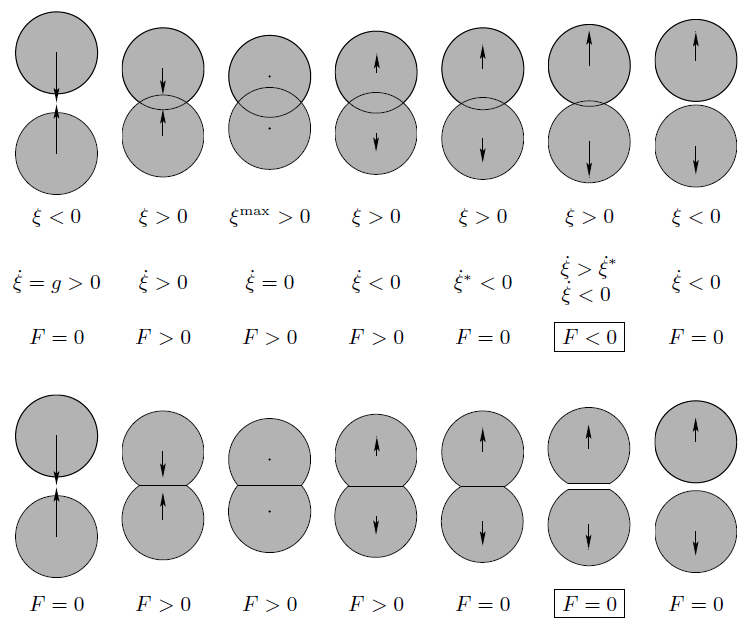
\includegraphics[width=0.9\textwidth]{images/mathematical_model/particle_attraction.PNG}
	% {\centerline{\includegraphics[scale=#2]{#1}}}
	% \vspace{-0.2cm}
	\label{fig:particle_attraction}
	\source{\adapted{\citeonline[p. 22]{bib:computational_granular_dynamics}}}
	% \vspace{-1cm}
\end{figure}

No entanto a atração entre partículas geralmente não condiz com resultados experimentais. Uma das técnicas para eliminar esse fenômeno é limitarem-se inferiormente as forças calculadas. Esse artifício justifica-se pois, embora tenha sido feita a hipótese de que as partículas sejam corpos rígidos, partículas reais são deformáveis, e essa deformação pode ser suficiente para encerrar a colisão em um tempo anterior àquele considerado pelo modelo de partículas rígidas. Isso é representado na figura \ref{fig:particle_attraction}.

Para o amortecedor linear, isso significa que
\begin{equation} \label{eq:corrected_linear_dashpot:normal_force}
	\normalForceScalarji = \max\Bqty{\elasticModulusij\cdot\overlapij + \normalDampingConstantij\cdot\overlapDerivativeij, \,\, 0},
\end{equation}
enquanto, para o modelo de esferas viscoelásticas, essa correção resulta em
\begin{equation*}
	\normalForceScalarji = \max\Bqty{\dfrac{4}{3}\ \effectiveNormalElasticij\ \sqrt{\effectiveRadiusij}\cdot\pqty{
		\overlapij^{\sfrac{3}{2}} + \normalDissipativeConstantij\ \overlapDerivativeij\ \sqrt{\overlapij}
	}, \,\, 0}.
\end{equation*}

Como consequência dessa mudança, o coeficiente de restituição normal tem seu valor alterado. \citeonline{bib:linear_dashpot_revisited} demonstram que, para o modelo de amortecedor linear, o coeficiente de restituição normal fica
\begin{equation} \label{eq:corrected_linear_dashpot:coefficient_of_restitution}
	\normalCoefficientOfRestitutionij = 
	\left\lbrace
		\def\arraystretch{1.8}
		\begin{array}{ll}
			\exp\bqty{-\dfrac{\betaij}{\omegaij}\pqty{\pi - \arctan\dfrac{2\ \betaij\ \omegaij}{\omegaij^2-\betaij^2}}}, & \text{se } \betaij < \dfrac{\omegazij}{\sqrt{2}} \\
			\exp\bqty{-\dfrac{\betaij}{\omegaij}\arctan\dfrac{2\ \betaij\ \omegaij}{\omegaij^2-\betaij^2}}, & \text{se } \betaij \in \bqty{\dfrac{\omegazij}{\sqrt{2}}, \omegazij} \\
			\exp\bqty{-\dfrac{\betaij}{\Omegaij} \ln\dfrac{\betaij + \Omegaij}{\betaij - \Omegaij}}, & \text{se } \betaij > \omegazij
		\end{array}
	\right.
	,
\end{equation}
em que
\begin{equation*}
	\def\arraystretch{1.5}
	\begin{array}{cc}
		\pqty{\omegazij}^2 = \bigslant{\elasticModulusij}{\massij}, &
		\betaij = \bigslant{\normalDampingConstantij}{\pqty{2\ \massij}}, \\
		\omegaij = \sqrt{\pqty{\omegazij}^2 - \betaij^2}, &	\Omegaij = \sqrt{\betaij^2 - \pqty{\omegazij}^2}.
	\end{array}
\end{equation*}

Uma expressão para o coeficiente de restituição corrigido para o modelo de esferas viscoelásticas pode ser encontrada em \citeonline{bib:schwager2008}.

\subsection{Modelos de Força Tangencial} \label{subsec:tangential_force_models}

Modelos para forças tangenciais, diferentemente dos modelos para forças normais, têm caráter intrinsecamente dinâmico, resistindo sempre ao movimento relativo entre as partículas. Esses modelos são responsáveis por fornecer um valor de força tangencial
\begin{equation*}
	\tangentialForceji = \tangentialForceScalarji\tangentialVersorji.
\end{equation*}

O fato de que essa força resiste ao movimento é representado pela desigualdade
\begin{equation*}
	\tangentialForceScalarji \leq 0.
\end{equation*}

Ainda, pela lei de Coulomb, a força tangencial não pode superar, em módulo, a força de atrito dinâmico 
\begin{equation*}
	\dynamicFrictionForceji = - \dynamicFrictionij\normalForceScalarji\cdot\tangentialVersorji,
\end{equation*}
em que \(\dynamicFrictionij\) é o coeficiente de atrito dinâmico entre o par de partículas \(\particlei\) e \(\particlej\). Disso segue a desigualdade
\begin{equation} \label{eq:coulomb_law}
	\tangentialForceScalarji \geq - \dynamicFrictionij\normalForceScalarji.
\end{equation}

Ao se determinar a força tangencial, a componente de torque \(\torqueji\) que a partícula \(j\) aplica sobre a \(i\) pode ser calculada como
\begin{equation*}
	\torqueji = \contactVectorij\cross\tangentialForceji
\end{equation*}

Nesta seção, são apresentados os dois principais modelos de força tangencial, de acordo com \citeonline{bib:computational_granular_dynamics}.

\subsubsection*{Modelo de Haff e Werner}

O modelo de Haff e Werner já foi aplicado com sucesso em diversas simulações. Esse modelo é o análogo tangencial do modelo de amortecedor linear para a força normal \cite{bib:computational_granular_dynamics}.

Para partículas esféricas, supondo que há contato, a equação \eqref{eq:overlap_derivative_and_normal_relative_velocity} sugere a analogia
\begin{equation*}
	\overlapDerivativeij \to \relativeTangentialVelocityScalarij
\end{equation*}

Além disso, devido ao caráter dinâmico da força tangencial, desconsideram-se componentes elásticas.

Com essas considerações e com a restrição da lei de Coulomb \eqref{eq:coulomb_law}, o análogo tangencial da equação \eqref{eq:linear_dashpot_force} fica
\begin{equation} \label{eq:haff_werner}
	\tangentialForceScalarji = - \min\set{\tangentialDampingConstantij\cdot\relativeTangentialVelocityScalarij,\,\, \dynamicFrictionij\cdot\normalForceScalarji},
\end{equation}
em que
\begin{itemize}
	\item \(\tangentialDampingConstantij\) é a constante de amortecimento tangencial efetiva do par \(i\) e \(j\). Essa constante pode ser obtida por uma associação em série de amortecedores de constantes \(\tangentialDampingConstanti\) e \(\tangentialDampingConstantj\), cada um pertencente a uma das partículas, como
	\begin{equation*}
		\tangentialDampingConstantij = \pqty{\dfrac{1}{\tangentialDampingConstanti} + \dfrac{1}{\tangentialDampingConstantj}}^{-1}
	\end{equation*}

	\item \(\dynamicFrictionij\) é o fator de atrito para o par \(\pqty{i,j}\). Embora esse fator seja definido para pares de partículas, é possível atribuirem-se fatores \(\dynamicFrictioni\) e \(\dynamicFrictionj\), um a cada partícula, de modo que
	\begin{equation*}
		\dynamicFrictionij = \min\Bqty{\dynamicFrictioni, \dynamicFrictionj}
	\end{equation*}
\end{itemize}

Com isso, o modelo de Haff e Werner assemelha-se a um modelo de amortecedor linear, exceto pelos fatos de haver a limitação da lei de Coulomb e de se desconsiderar a componente elástica.

A dificuldade apresentada por esse modelo é que não há propriedades de material mensuráveis a partir dos quais se possa extrair os valores de \(\tangentialDampingConstanti\) e \(\tangentialDampingConstantj\). Esses parâmetros só são conhecidos posteriormente, com a comparação entre os resultados das simulações e experimentos.

\subsubsection*{Modelo de Cundall e Strack}

Ao contrário do modelo de Haff e Werner, no modelo de Cundall e Strack supõe a existência de uma mola que resiste ao deslocamento relativo entre as partículas na direção tangencial. Esse modelo foi proposto por \citeonline[p. 52]{bib:cundall1979}. Considera-se que a mola esteja na posição de equilíbrio no instante de início da colisão \(\collisionBeginningij\), e a sua deformação ou elongação no instante \(t\) é dada por
\begin{equation*}
	\elongationij\pqty{t} = \int_{\collisionBeginningij}^{t} \relativeTangentialVelocityScalarij\pqty{\tau} \dd{\tau}.
\end{equation*}

Com isso, e considerando a restrição da lei de Coulomb, a força calculada pelo modelo de Cundall e Strack fica
\begin{equation*}
	\tangentialForceScalarji = - \min\Bqty{\tangentialElasticConstantij\elongationij,\,\, \dynamicFrictionij\cdot\normalForceScalarji},
\end{equation*}
sendo que
\begin{itemize}
	\item \(\tangentialElasticConstantij\) é a constante elástica da mola equivalente no choque. Essa mola pode ser tratada como a associação em série de molas de constantes \(\tangentialElasticConstanti\) e \(\tangentialElasticConstantj\), cada uma pertencente à respectiva partícula:
	\begin{equation*}
		\tangentialElasticConstantij = \pqty{\dfrac{1}{\tangentialElasticConstanti} + \dfrac{1}{\tangentialElasticConstantj}}^{-1}.
	\end{equation*}

	Porém essas constantes, assim como o amortecimento no modelo de Haff e Werner, só são obtidas na comparação posterior das simulações com resultados experimentais.
\end{itemize}

\section{Algoritmo de Gear} \label{sec:gear_integration_scheme}

Com as equações diferenciais bem determinadas através do uso de modelos de interação, inicia-se a busca por sua solução. O algoritmo de Gear é um método de resolução de equações diferenciais ordinárias originado do trabalho de \citeonline{bib:gear_book}.

Gear considerou o problema de extrapolar funções sujeitas a equações diferenciais. Dada uma função \(y\) tal que \(y(t), \deriv{1}{y}(t),\dotsc, \deriv{\taylorOrder}{y}(t)\) existem e são bem conhecidos, o objetivo é determinar os valores de \(y(t + \Dt), \deriv{1}{y}(t + \Dt),\dotsc, \deriv{\taylorOrder}{y}(t + \Dt)\) sabendo que \(y\) deve satisfazer uma equação diferencial da forma
\begin{equation} \label{eq:gear_diff}
	\deriv{\eqOrder}{y} = \eqFor{y}\pqty{y, \deriv{1}{y},\dotsc,\deriv{\eqOrder-1}{y}, t}
\end{equation}
com \(\eqOrder \leq \taylorOrder\).

O algoritmo consiste em duas etapas: uma etapa de \textit{previsão} e uma de \textit{correção}, detalhadas nas seções \ref{subsec:prediction} e \ref{subsec:correction}.

\subsection{Etapa de Predição} \label{subsec:prediction}

Nos métodos computacionais desenvolvidos para a solução dessas equações, a extrapolação de funções possui um papel fundamental por permitir a estimativa de valores além do conjunto previamente conhecido.

A etapa de predição é responsável por obter uma estimativa para \(y\pqty{t+\Dt}\), \(\deriv{1}{y}\pqty{t+\Dt}\),\,\dots, \(\deriv{\taylorOrder}{y}\pqty{t+\Dt}\) através de uma extrapolação a partir dos valores de \(y\pqty{t}\), \(\deriv{1}{y}\pqty{t}\),\(\dotsc\), \(\deriv{\taylorOrder}{y}\pqty{t}\).

Para simplificação da notação, dada uma função \(y\), define-se o vetor das \(\taylorOrder\) primeiras derivadas de \(y\) como a função vetorial
\begin{equation*}
	\drvvec{\taylorOrder}{y} = \pqty{y, \deriv{1}{y}, \deriv{2}{y}, \dotsc, \deriv{\taylorOrder}{y}}
\end{equation*}
nos pontos em que todas as coordenadas estiverem definidas.

Conforme demonstrado por \citeonline{bib:extrapolation}, métodos de extrapolação lineares para uma função e suas derivadas podem ser escritos na forma
\begin{equation*}
	\begin{pmatrix}
		\predicted{y} \\
		\predicted{\deriv{1}{y}} \\
		\predicted{\deriv{2}{y}} \\
		\vdots \\
		\predicted{\deriv{\taylorOrder-1}{y}} \\
		\predicted{\deriv{\taylorOrder}{y}}
	\end{pmatrix}
	=
	\begin{pmatrix}
		a_{0,0} & a_{0,1} & a_{0,2} &  & a_{0,\taylorOrder-1} & a_{0,\taylorOrder} \\
		a_{1,0} & a_{1,1} & a_{1,2} & \cdots & a_{1,\taylorOrder-1} & a_{1,\taylorOrder} \\
		a_{2,0} & a_{2,1} & a_{2,2} &  & a_{2,\taylorOrder-1} & a_{2,\taylorOrder} \\
	     & \vdots & & \ddots & & \vdots \\
	    a_{\taylorOrder-1,0} & a_{\taylorOrder-1,1} & a_{\taylorOrder-1,2} &  & a_{\taylorOrder-1,\taylorOrder-1} & a_{\taylorOrder-1,\taylorOrder} \\
	    a_{\taylorOrder,0} & a_{\taylorOrder,1} & a_{\taylorOrder,2} & \cdots & a_{\taylorOrder,\taylorOrder-1} & a_{\taylorOrder,\taylorOrder}
	\end{pmatrix}
	\cdot
	\begin{pmatrix}
		y \\
		\deriv{1}{y} \\
		\deriv{2}{y} \\
		\vdots \\
		\deriv{\taylorOrder-1}{y} \\
		\deriv{\taylorOrder}{y}
	\end{pmatrix}
\end{equation*}
ou, mais simplesmente,
\begin{equation} \label{eq:prediction}
	\drvvec{\taylorOrder}{\predicted{y}} = \extrapolationMatrix{\taylorOrder} \cdot \drvvec{\taylorOrder}{y}.
\end{equation}
em que a matriz \(\extrapolationMatrix{\taylorOrder}\) é determinada pelo método escolhido e \(\drvvec{\taylorOrder}{\predicted{y}}\) é o vetor de derivadas de \(y\) \textit{predito}.

Dentre os métodos de extrapolação mais utilizados estão o método de expansão de Taylor, o método de Richardson, o método de interpolação de Aitken e os métodos de Runge-Kutta, cada qual com diferentes características em termos de exatidão e estabilidade \cite{bib:gear_book}.

O método de extrapolação por expansão de Taylor combina simplicidade, exatidão e estabilidade, e por isso é o método adotado neste trabalho. Esse método é fundamentado pelo \nameref{theo:taylor}.

\begin{unnumberedtheorem}[Teorema  de Taylor] \label{theo:taylor}
	Seja \(y\) uma função de uma variável com derivadas \(\deriv{1}{y},\dotsc,y^{\pqty{\taylorOrder+1}}\) todas definidas em um intervalo aberto que contenha \(t\), e seja \(\remainderFunction{\taylorOrder}{t}{y}\) definida pela equação
    \begin{equation*}
    	y(t + \Dt) = y(t) + \deriv{1}{y}(t)\cdot\Dt + \dotsb + \dfrac{\deriv{\taylorOrder}{y}(t)}{\taylorOrder!}\cdot\Dt^\taylorOrder + \remainderFunction{\taylorOrder}{t}{y}(\Dt).
    \end{equation*}
    Então
    \begin{equation} \label{eq:remainder_limit}
    	\lim_{\Dt \rightarrow 0} \dfrac{\remainderFunction{\taylorOrder}{t}{y}(\Dt)}{\Dt^\taylorOrder} = 0.
    \end{equation}
\end{unnumberedtheorem}

Uma versão mais completa desse teorema é apresentada e demonstrada por \citeonline{bib:spivak}.

A função \(\remainderFunction{\taylorOrder}{t}{y}\) é o resto de ordem \(\taylorOrder\) para a função \(y\) no entorno de \(t\). A equação \eqref{eq:remainder_limit} indica que o resto é um termo da ordem de \(\Dt^{\taylorOrder+1}\), e motiva a aproximação
\begin{equation} \label{eq:taylor_trunc}
    y(t + \Dt) \approximately y(t) + \deriv{1}{y}(t)\cdot\Dt + \dotsb + \dfrac{\deriv{\taylorOrder}{y}(t)}{\taylorOrder!}\cdot\Dt^\taylorOrder.
\end{equation}

A equação \eqref{eq:taylor_trunc} é o truncamento da expansão de Taylor na \(\taylorOrder\)-ésima derivada.

Considerando uma função vetorial \(\vec{y}:I\subseteq \real \rightarrow \real^m\), o \nameref{theo:taylor} pode ser aplicado a cada uma de suas funções coordenadas\footnote{Escrevendo \(\vec{y}(t) = \pqty{y_1(t),\dotsc,y_m(t)}\), a \(i\)-ésima função coordenada de \(\vec{y}\) é a função \(y_i\).}, resultando em uma expansão similar à da equação \eqref{eq:taylor_trunc}, desde que as hipóteses do teorema sejam satisfeitas. Os casos de interesse são \(m=1\), para funções reais; \(m=2\), para vetores bidimensionais como a posição de uma partícula em uma simulação em duas dimensões; \(m=3\), para simulações em três dimensões; e \(m=4\) para algumas parametrizações para a orientação das partículas, como mostrado no \autoref{app:three_dimensional_rotation}.

Assim, o \nameref{theo:taylor} permite a estimativa do valor de uma função em um ponto \(t+\Dt\) a partir do valor da função e de suas derivadas em um ponto \(t\), e essa estimativa é tanto melhor quanto menor for o valor de \(\Dt\).

Não somente a função pode ser prevista, mas suas derivadas também. Para a \(j\)-ésima derivada de \(y\):
\begin{equation*}
	\predicted{\deriv{j}{y}}\pqty{t + \Dt} = \deriv{j}{y}\pqty{t} + \dotsb + \dfrac{\Dt^{\taylorOrder-j}}{\pqty{\taylorOrder-j}!}\cdot\deriv{\taylorOrder-j}{y}\pqty{t}.
\end{equation*}

Com isso, é possível escrever
\begin{equation} \label{eq:extrapolation_matricial_form}
	\def\arraystretch{1.2}
\begin{pmatrix}
	\predicted{y} \\
	\predicted{\deriv{1}{y}} \\
	\predicted{\deriv{2}{y}} \\
	\vdots \\
	\predicted{\deriv{\taylorOrder-1}{y}} \\
	\predicted{\deriv{\taylorOrder}{y}}
\end{pmatrix}
=
\begin{pmatrix}
	1 & \Dt & \frac{\Dt^2}{2} &  & \frac{\Dt^{\taylorOrder-1}}{\pqty{\taylorOrder-1}!} & \frac{\Dt^\taylorOrder}{\taylorOrder!} \\
	0 & 1 & \Dt & \cdots & \frac{\Dt^{\taylorOrder-2}}{\pqty{\taylorOrder-2}!} & \frac{\Dt^{\taylorOrder-1}}{\pqty{\taylorOrder-1}!} \\
	0 & 0 & 1 &  & \frac{\Dt^{\taylorOrder-3}}{\pqty{\taylorOrder-3}!} & \frac{\Dt^{\taylorOrder-2}}{\pqty{\taylorOrder-2}!} \\
     & \vdots & & \ddots & & \vdots \\
    0 & 0 & 0 &  & 1 & \Dt \\
    0 & 0 & 0 & \cdots & 0 & 1
\end{pmatrix}
\cdot
\begin{pmatrix}
	y \\
	\deriv{1}{y} \\
	\deriv{2}{y} \\
	\vdots \\
	\deriv{\taylorOrder-1}{y} \\
	\deriv{\taylorOrder}{y}
\end{pmatrix}.
\end{equation}

A matriz da equação \eqref{eq:extrapolation_matricial_form} é a matriz de extrapolação do método de expansão de Taylor, sendo a mesma para a extrapolação de ordem \(\taylorOrder\) de qualquer função.

Esse método ainda pode ser usado para aproximar as funções de posição e de orientação da partícula, assim como outros graus de liberdade que o problema porventura possua.

Todavia essa predição geralmente não é exata. Uma das razões para isto é que o truncamento da expansão de Taylor, ou qualquer outro método de extrapolação que se use, despreza a função resto, que não é necessariamente nula. Mesmo assim, essa diferença é aceitável quando se utilizam passos de tempo suficientemente pequenos. 

A principal fonte de erros da equação \eqref{eq:extrapolation_matricial_form} é que não se considera, em nenhum momento, equações diferenciais a que a função \(y\) pode estar restrita. Por exemplo, para a posição ou a orientação de uma partícula, pode haver a ação de forças e torques atuantes entre os instantes \(t\) e \(t + \Dt\). É necessário, então, \textit{corrigir} a função prevista. Essa correção pode ser feita na etapa de correção, apresentada na seção \ref{subsec:correction}.

\subsection{Correção} \label{subsec:correction}

Na etapa de correção, um termo é adicionado ao vetor previsto \(\drvvec{\taylorOrder}{\predicted{y}}\) para se obter o vetor \(\drvvec{\taylorOrder}{\corrected{y}}\), corrigido em função da equação diferencial \eqref{eq:gear_diff}.

O valor corrigido para \(\deriv{\eqOrder}{y}\) pode ser obtido no instante \(t+\Dt\) diretamente através da equação:
\[
	\corrected{\deriv{\eqOrder}{y}}\pqty{t+\Dt} = \eqFor{y}\pqty{\predicted{y}, \predicted{\deriv{1}{y}},\dotsc,\predicted{\deriv{\eqOrder-1}{y}}, t+\Dt},
\]
e assim é conhecido o valor do erro \(\Delta \deriv{\eqOrder}{y} \eqdef \corrected{\deriv{\eqOrder}{y}} - \predicted{\deriv{\eqOrder}{y}}\) no ponto \(t+\Dt\).

Como demonstrado por \citeonline{bib:gear_book}, as demais derivadas de \(y\) podem ser corrigidas em função de \(\Delta \deriv{\eqOrder}{y}\) de acordo com a equação
\begin{equation} \label{eq:correction}
	\def\arraystretch{1.2}
	\begin{pmatrix}
		\corrected{\deriv{0}{y}} \\
		\corrected{\deriv{1}{y}} \\
		\corrected{\deriv{2}{y}} \\
		\vdots \\
		\corrected{\deriv{\eqOrder}{y}} \\
		\vdots \\
		\corrected{\deriv{\taylorOrder-1}{y}} \\
		\corrected{\deriv{\taylorOrder}{y}}
	\end{pmatrix}
	=
	\begin{pmatrix}
		\predicted{\deriv{0}{y}} \\
		\predicted{\deriv{1}{y}} \\
		\predicted{\deriv{2}{y}} \\
		\vdots \\
		\predicted{\deriv{\eqOrder}{y}} \\
		\vdots \\
		\predicted{\deriv{\taylorOrder-1}{y}} \\
		\predicted{\deriv{\taylorOrder}{y}}
	\end{pmatrix}
	+
	\begin{pmatrix}
		\correctorConstant{0}{\eqOrder} \\
		\correctorConstant{1}{\eqOrder}\frac{1}{\Dt} \\
		\correctorConstant{2}{\eqOrder}\frac{2}{\Dt^2} \\
		\vdots \\
		\correctorConstant{\eqOrder}{\eqOrder}\frac{\eqOrder!}{\Dt^\eqOrder}\\
		\vdots \\
		\correctorConstant{\taylorOrder-1}{\eqOrder}\frac{\pqty{\taylorOrder-1}!}{\Dt^{\taylorOrder-1}}\\
		\correctorConstant{\taylorOrder}{\eqOrder}\frac{\taylorOrder!}{\Dt^\taylorOrder}
	\end{pmatrix}
	\cdot
	\dfrac{\Dt^\eqOrder}{\eqOrder!}\Delta \deriv{\eqOrder}{y},
\end{equation}
sendo que as constantes corretoras \(\correctorConstant{0}{\eqOrder}\), \(\correctorConstant{1}{\eqOrder}\), \(\dotsc\), \(\correctorConstant{\taylorOrder}{\eqOrder}\) dependem da ordem \(\taylorOrder\) da maior derivada considerada e da ordem \(\eqOrder\) da equação diferencial. Alguns dos valores dessas constantes são apresentados na tabela \ref{table:corrector_constants}. Em todos casos, sempre se tem que \(\correctorConstant{\eqOrder}{\eqOrder}=1\), pois \(\corrected{\deriv{p}{y}} = \predicted{\deriv{p}{y}} + \Delta \deriv{\eqOrder}{y}\).

Por simplicidade, escreve-se
\begin{equation*}
	\correctorConstantVector{\taylorOrder}{\eqOrder} = \pqty{\correctorConstant{0}{\eqOrder}, \correctorConstant{1}{\eqOrder}\dfrac{1}{\Dt}, \correctorConstant{2}{\eqOrder}\frac{2}{\Dt^2}, \dotsc, \correctorConstant{\taylorOrder}{\eqOrder}\frac{\taylorOrder!}{\Dt^\taylorOrder}},
\end{equation*}
e então a equação \eqref{eq:correction} pode ser reescrita como
\begin{equation} \label{eq:correction_simplified}
	\drvvec{\taylorOrder}{\corrected{y}} = \drvvec{\taylorOrder}{\predicted{y}} + \correctorConstantVector{\taylorOrder}{\eqOrder}\cdot\dfrac{\Dt^\eqOrder}{\eqOrder!}\Delta \deriv{\eqOrder}{y}.
\end{equation}
	
\begin{table}[h]
	\caption{Constantes corretoras para o algoritmo de Gear em função da ordem \(\taylorOrder\) da maior derivada considerada e da ordem \(\eqOrder\) da equação diferencial}
	\label{table:corrector_constants}

	\begin{equation*}
		% \arraycolsep=1.4pt
		\def\arraystretch{1.5}
		\begin{array}{cccccccccc}
	\hline
	\hline
		\eqOrder & \taylorOrder & \correctorConstant{0}{\eqOrder} & \correctorConstant{1}{\eqOrder} & \correctorConstant{2}{\eqOrder} & \correctorConstant{3}{\eqOrder} & \correctorConstant{4}{\eqOrder} & \correctorConstant{5}{\eqOrder} & \correctorConstant{6}{\eqOrder} & \correctorConstant{7}{\eqOrder} \\
	\hline
		\multirow{6}{*}{1} 
		& 2 & \frac{5}{12} & 1 & \frac{1}{2} & \emptyTableEntry & \emptyTableEntry & \emptyTableEntry & \emptyTableEntry & \emptyTableEntry \\
		& 3 & \frac{3}{8} & 1 & \frac{3}{4} & \frac{1}{6} & \emptyTableEntry & \emptyTableEntry & \emptyTableEntry & \emptyTableEntry \\
		& 4 & \frac{251}{720} & 1 & \frac{11}{12} & \frac{1}{3} & \frac{1}{24} & \emptyTableEntry & \emptyTableEntry & \emptyTableEntry \\
		& 5 & \frac{95}{288} & 1 & \frac{25}{24} & \frac{35}{72} & \frac{5}{48} & \frac{1}{120} & \emptyTableEntry & \emptyTableEntry \\
		& 6 & \frac{19087}{60480} & 1 & \frac{137}{120} & \frac{5}{8} & \frac{17}{96} & \frac{1}{40} & \frac{1}{720} & \emptyTableEntry \\
		& 7 & \frac{5257}{17280} & 1 & \frac{49}{40} & \frac{203}{270} & \frac{49}{192} & \frac{7}{144} & \frac{7}{1440} & \frac{1}{5040} \\
	\hline
		\multirow{5}{*}{2} 
		& 3 & \frac{1}{6} & \frac{5}{6} & 1 & \frac{1}{3} & \emptyTableEntry & \emptyTableEntry & \emptyTableEntry & \emptyTableEntry \\
		& 4 & \frac{19}{120} & \frac{3}{4} & 1 & \frac{1}{2} & \frac{1}{12} & \emptyTableEntry & \emptyTableEntry & \emptyTableEntry \\
		& 5 & \frac{3}{20} & \frac{251}{360} & 1 & \frac{11}{18} & \frac{1}{6} & \frac{1}{60} & \emptyTableEntry & \emptyTableEntry \\
		& 6 & \frac{863}{6048} & \frac{665}{1008} & 1 & \frac{25}{36} & \frac{35}{144} & \frac{1}{24} & \frac{1}{360} & \emptyTableEntry \\
		& 7 & \frac{1925}{14112} & \frac{19087}{30240} & 1 & \frac{137}{180} & \frac{5}{16} & \frac{17}{240} & \frac{1}{120} & \frac{1}{2520} \\
	\hline
		\multirow{4}{*}{3} 
		& 4 & \frac{1}{4} & \frac{1}{2} & \frac{5}{4} & 1 & \frac{1}{4} & \emptyTableEntry & \emptyTableEntry & \emptyTableEntry \\
		& 5 & \frac{3}{80} & \frac{19}{40} & \frac{9}{8} & 1 & \frac{3}{8} & \frac{1}{20} & \emptyTableEntry & \emptyTableEntry \\
		& 6 & \frac{221}{5040} & \frac{9}{20} & \frac{251}{240} & 1 & \frac{11}{24} & \frac{1}{10} & \frac{1}{120} & \emptyTableEntry \\
		& 7 & \frac{2185}{46368} & \frac{863}{2016} & \frac{95}{96} & 1 & \frac{25}{48} & \frac{49}{336} & \frac{1}{48} & \frac{1}{840} \\
	\hline
		\multirow{3}{*}{4} 
		& 5 & \frac{1}{30} & \frac{1}{10} & 1 & \frac{5}{3} & 1 & \frac{1}{5} & \emptyTableEntry & \emptyTableEntry \\
		& 6 & \frac{16}{630} & \frac{3}{20} & \frac{19}{20} & \frac{3}{2} & 1 & \frac{3}{10} & \frac{1}{30} & \emptyTableEntry \\
		& 7 & \frac{11}{630} & \frac{221}{1260} & \frac{9}{10} & \frac{251}{180} & 1 & \frac{11}{30} & \frac{1}{15} & \frac{1}{210} \\
	\hline
	\hline	
		\end{array}
	\end{equation*}
	\source{\citeonline{bib:gear_book}}
\end{table}

\alert{O \(k\) que estou usando é diferente do de Gear. Para Gear, a maior derivada considerada é \(k-1\). A minha tabela está corrigida e, em todos os casos, \(k_{\text{Ruan}} = k_{\text{Gear}}-1 \). Será que devo mudar o símbolo?}

Ainda, de acordo com \citeonline[p. 153]{bib:gear_book}, o erro global do algoritmo é da ordem de \(\Dt^{\taylorOrder+1+\maxDerivOrder-\eqOrder}\), em que \(\maxDerivOrder\) é o maior inteiro tal que a equação diferencial \eqref{eq:gear_diff} pode ser escrita como
\begin{equation} \label{eq:smaller_diff}
	\deriv{\eqOrder}{y} = \eqFor{y}\pqty{y, \deriv{1}{y},\dotsc,\deriv{\eqOrder-\maxDerivOrder}{y}, t}.
\end{equation}

E, com isso, a etapa de correção está bem definida. Em virtude das características apresentadas, o algoritmo de Gear é usado como método de resolução das equações de movimento dos elementos dos sistemas de partículas.

Com as considerações feitas neste capítulo, todas as ferramentas matemáticas necessárias para a solução do problema já estão expostas. A próxima etapa, então, é desenvolver um método numérico que permita a implementação desse algoritmo de solução.

% \subsection{Aplicação do Algoritmo de Gear aos Sistemas de Partículas} \label{subsec:gear_application}

%  Esta seção é dedicada a apresentar essa utilização. Primeiramente, é apresentado o caso geral. Por fim, mostra-se a simplificação existente para partículas esféricas.



% E assim está demonstrada a aplicação do algoritmo de Gear aos sistemas de partículas. 

% Para o caso da posição de uma partícula  \(\particlei\), a equação de movimento translacional é obtida a partir do princípio da superposição \eqref{eq:superposition_translation} e da primeira lei de Euler \eqref{eq:motion_first} como
% \begin{equation*}
% 	\accelerationi = \dfrac{1}{\massi}\sum_{\particlej\in\neighborhoodi}\forceji.
% \end{equation*}

% A força \(\forceji\) que cada partícula \(\particlej\) aplica sobre \(\particlei\) é função de suas posições, velocidades, orientações e velocidades angulares. Utilizando-se parametrizações \(\orientationi\) e \(\orientationj\) para as orientações das partículas, obtém-se
% \begin{equation*}
% 	\accelerationi = \dfrac{1}{\massi}\sum_{\particlej\in\neighborhoodi}\forceji\pqty{\positioni, \velocityi, \orientationi, \deriv{1}{\orientationi}, \positionj, \velocityj, \orientationj, \deriv{1}{\orientationj}}.
% \end{equation*}

% De forma semelhante, a equação de movimento rotacional para \(\particlei\) é obtida a partir do princípio da superposição \eqref{eq:superposition_rotation} e da equação diferencial para rotação parametrizada \eqref{eq:diff_equation_orientation_parametrization}, como apresentada na \autoref{subsubsec:general_rotation}:
% \begin{equation*}
% 	\deriv{2}{\orientationi} = \eqFori{\orientation}\pqty{\sum_{\particlej\in\neighborhoodi}\torqueji, \,\orientationi,\,\deriv{1}{\orientationi}}.
% \end{equation*}

% Ainda, cada parcela \(\torqueji\) é função das coordenadas (e suas derivadas) das partículas \(\particlei\) e \(\particlej\), e então
% \begin{equation*}
% 	\deriv{2}{\orientationi} = \eqFori{\orientation}\pqty{\sum_{\particlej\in\neighborhoodi}\torqueji\pqty{\positioni, \velocityi, \orientationi, \deriv{1}{\orientationi}, \positionj, \velocityj, \orientationj, \deriv{1}{\orientationj}}, \,\orientationi,\,\deriv{1}{\orientationi}}.
% \end{equation*}

% Para se utilizar o algoritmo de Gear, porém, é necessário escrever-se uma equação diferencial para uma única função, e o que se tem, até agora, é um sistema de \(\numberOfParticles\) equações
% \begin{equation*}
% 	,
% \end{equation*}
% em que \(\numberOfParticles\) é o número de partículas no sistema.

% \alert{Apagar a partir daqui}
% ou, vendo \(\angularVelocityi\), \(\positionj\), \(\velocityj\) e \(\angularVelocityj\) como funções do tempo,
% \begin{equation*}
% 	\accelerationi = \dfrac{1}{\massi}\sum_{\particlej\in\neighborhoodi}\forceji\pqty{\positioni, \velocityi, t}.
% \end{equation*}

% Já a equação de movimento rotacional é obtida através de \eqref{eq:superposition_rotation} e \eqref{eq:rotation_spherical_particle} como
% \begin{equation*}
% 	\angularAccelerationi = \dfrac{1}{\momentOfInertiai}\sum_{\particlej\in\neighborhoodi}\torqueji\pqty{\positioni, \velocityi, \angularVelocityi, \positionj, \velocityj, \angularVelocityj},
% \end{equation*}
% ou, similarmente,
% \begin{equation*}
% 	\angularAccelerationi = \dfrac{1}{\momentOfInertiai}\sum_{\particlej\in\neighborhoodi}\torqueji\pqty{\angularVelocityi, t}.
% \end{equation*}

% Assim, para o movimento de translação, a ordem da equação diferencial resultante é \(p=2\), enquanto \(q=1\) na equação \eqref{eq:smaller_diff}. Disso que resulta que o erro do algoritmo é da ordem de \(\Dt^{\taylorOrder}\).

% Por sua vez, a equação para o movimento de rotação tem ordem \(p=1\), e pode-se considerar que \(q=0\) em \eqref{eq:smaller_diff}. Logo, o erro também é da ordem de \(\Dt^{\taylorOrder}\).
\chapter{O Método de Elementos Discretos} \label{ch:discrete_element_method}

\alert{Descrever aqui as características básicas e gerais que o \DEM{} possui}

\alert{Falar das forças externas, que são fundamentais para algumas das simulações}

\alert{Mostrar os principais aspectos do algoritmo e passar por cada um deles, detalhando}

\alert{Falar do critério de parada}

O Método de Elementos Discretos (\DEM{}\footnote{Do inglês, \textit{Discrete Element Method}.}) refere-se a uma família de métodos numéricos aplicados na simulação de sistemas de partículas. Esses métodos compartilham diversas características entre si, como o monitoramento da vizinhança de cada partícula, o cálculo explícito das variáveis do problema a partir de seus valores nos instantes anteriores, dentre outras.

Este capítulo é dedicado à apresentação e à explicação dessas características. São apresentados o funcionamento geral de um algoritmo \DEM{}, o procedimento de solução das equações do problema e as principais etapas do método.

\alert{Talvez descrever melhor o que há em cada seção}

\section{Características Gerais do Método}

Segundo \citeonline[p. 1]{bib:bicanic2007}, o \DEM{} constitui-se de técnicas de modelagem computacional indicadas para a simulação do comportamento dinâmico de conjuntos de partículas de geometria arbitrária sujeitas a restrições de contato variantes no tempo.

Conforme a definição apresentada por \apudonline{bib:cundall1989}{bib:bicanic2007}, métodos de elementos discretos são métodos computacionais que:
\begin{alineas}
	\item consideram deslocamentos e rotações finitos de corpos discretos;
	\item reconhecem novos contatos automaticamente à medida que a simulação progride.
\end{alineas}

Cada partícula é considerada um corpo rígido com seis graus de liberdade: três translações e três rotações, e está sujeita às equações diferenciais de movimento descritas na \autoref{sec:equations_of_motion}. O processo de simulação consiste na solução dessas equações. 

Em um sistema, porém, os elementos interagem entre si, e as forças e os torques atuantes sobre eles dependem dessas interações. Sendo assim, é necessário o \textit{monitoramento das vizinhanças}, isto é, o método deve sempre determinar quais são os pares de elementos que interagem em cada passo de tempo. Dentre os algoritmos disponíveis, destacam-se o algoritmo de Verlet, dedicado a partículas esféricas, o algoritmo \textit{link cell} e o algoritmo \textit{lattice}. \alert{São esses mesmo que considero depois?}

Os elementos da simulação ainda podem pertencer a \textit{tipos} distintos. Por exemplo, é possível distinguirem-se \textit{partículas}, elementos cujas equações de movimento precisam ser resolvidas, de \textit{elementos de contorno}, que têm seu estado conhecido já na etapa de inicialização do algoritmo. Além dos elementos de contorno, outras \textit{condições de contorno} podem ser aplicadas ao sistema, como restrições de movimento, paredes reflexivas e condição de repetição.

De acordo com \citeonline[p. 2]{bib:bicanic2007}, existem diversas metodologias para a simulação com elementos discretos, sendo que as variações ocorrem:
\begin{alineas}
	\item nos algoritmos de detecção de contatos;
	\item nas formulações para as interações;
	\item nas condições de contorno;
	\item na consideração de modelos de fratura, fragmentação ou aglutinação;
	\item nos métodos de integração das equações;
	\item nos algoritmos de monitoramento de vizinhanças.
\end{alineas}

\subsection{Discretização Temporal}

Como é recorrente em métodos de simulação numérica, o \DEM{} conta com a discretização do tempo para a solução das equações de movimento. Para o intervalo de simulação \(\interval{\initialInstant}{\finalInstant}\), sendo \(\initialInstant\) o instante inicial e \(\finalInstant\), o final, uma discretização temporal é um conjunto \(\set{t_0, t_1, \dotsc, t_{\numberOfTimesteps}}\) tal que
\begin{equation*}
	\initialInstant = \instant[0] < \instant[1] < \dotsb < \instant[\numberOfTimesteps - 1] < \instant[\numberOfTimesteps] = \finalInstant.
\end{equation*}

O valor \(\numberOfTimesteps\) é o número de passos de tempo da simulação. Um passo de tempo é o período compreendido entre dois instantes consecutivos da discretização. A duração do \(n\)-ésimo passo de tempo é dada então por
\begin{equation*}
	\Dt[n] \eqdef \instant[n] - \instant[n-1],
\end{equation*}
e escreve-se \(\Dt\) no caso em que os passos de tempo têm todos a mesma duração.

Com isso, o objetivo do Método de Elementos Discretos torna-se obter a solução para as coordenadas das partículas no tempo discretizado.

\subsection{Solução das Equações}

A solução das equações governantes do sistema é feita conforme explicado na \autoref{subsec:motion_equations_solution} utilizando algoritmos de integração como o algoritmo de Gear, descrito na \autoref{sec:gear_integration_scheme}.

Uma característica dos métodos de elementos discretos é serem métodos explícitos, ou seja, o estado do sistema de partículas no instante \(\instant[n]\) é calculado a partir do estado em \(\instant[n-1]\) que se supõe ser conhecido. Isso é evidente no algoritmo de Gear.

De acordo com \citeonline{bib:computational_granular_dynamics}, a solução das equações pode ser dividida em quatro etapas, sendo elas:

\begin{enumdesc}
	\item[Determinação da Vizinhança:] Nessa etapa, a vizinhança de cada partícula do sistema é construída (no primeiro instante) ou atualizada (em instantes posteriores da simulação). O objetivo é limitar a quantidade de interações avaliadas no passo de tempo. 
	\item[Predição:] Nesse passo, o estado do sistema no instante \(\instant[n]\) é predito em função do estado em \(\instant[n-1]\). Essa predição é feita por métodos de extrapolação, como explicado na \autoref{subsec:prediction}.
	\item[Interação:] A partir do estado predito do sistema, são computadas as interações entre cada partícula e os elementos de sua vizinhança. \label{item:interaction}
	\item[Correção:] Na etapa de correção, o estado do sistema no instante \(\instant[n]\) é corrigido em função das interações calculadas na etapa \ref{item:interaction} e das equações governantes do problema, como apresentado na \autoref{subsec:correction}. Embora esse processo não seja exato, o DEM considera o estado corrigido como a solução do problema para o instante \(\instant[n]\).
\end{enumdesc}

\alert{é estranho colocar a vizinhança antes. Três motivos por que isso é feito: 1) a referência faz; 2) o passo de tempo que usamos é pequeno; 3) permite uma fácil alteração do algoritmo de integração da equação}

Sendo \(\instant[n]\) o instante de interesse e \(\instant[n-1]\), o instante anterior em que o sistema é conhecido, as posições e as orientações das partículas podem ser previstas como na equação \eqref{eq:position_and_orientation_prediction}:
\begin{equation*}
	\def\arraystretch{1.5}
	\begin{array}{c}
		\drvec{\taylorOrder}{\positionipr}\pqty{\instant[n]} = \extrapolationMatrix{\taylorOrder}[\Dt[n]]\cdot\drvec{\taylorOrder}{\positioni}\pqty{\instant[n-1]} \\
		\drvec{\taylorOrder}{\orientationipr}\pqty{\instant[n]} = \extrapolationMatrix{\taylorOrder}[\Dt[n]]\cdot\drvec{\taylorOrder}{\orientationi}\pqty{\instant[n-1]} \\
	\end{array}, \quad \particlei \in \particleSet,
\end{equation*}
sendo \(\particleSet\) o conjunto de partículas do sistema, \(\taylorOrder\), a ordem de extrapolação escolhida para o método e \(\extrapolationMatrix{\taylorOrder}[\Dt[n]]\), a matriz de extrapolação dada na equação \eqref{eq:extrapolation_matricial_form} calculada com o passo de tempo \(\Dt[n]\).

A vizinhança de uma partícula, como explicado na \autoref{sec:neighborhood}, é o conjunto de todas as entidades da simulação com as quais há interação. A vizinhança da \(i\)-ésima partícula do sistema é denotada por \(\neighborhoodi\) \alert{Verificar se essas coisas já não foram ditas antes com a mudança das seções.}. Cada elemento \(\elementj\) da vizinhança de \(\particlei\) contribui para a força \(\forcei\) e o torque \(\torquei\) resultantes sobre a mesma com parcelas \(\forceji\) e \(\torqueji\) que são, por hipótese, dependentes apenas do par \(\orderedPair{\particlei}{\elementj}\). Com isso, os vetores força e torque resultantes são calculados como
\begin{equation*}
	\def\arraystretch{1.5}
	\begin{array}{c}
		\displaystyle \forcei = \sum_{\elementj\in\neighborhoodi} \forceji \\
		\displaystyle \torquei = \sum_{\elementj\in\neighborhoodi} \torqueji 
	\end{array}, \quad \particlei \in \particleSet,
\end{equation*}
já incluindo-se as forças e os torques provenientes de elementos externos ao sistema.

A cada um dos graus de liberdade da partícula é associada uma equação que determina seu comportamento. Para as equações de movimento, essas equações são escritas na forma
\begin{equation*}
	\def\arraystretch{1.5}
	\begin{array}{c}
		\displaystyle \accelerationicorr =  \dfrac{1}{\massi}\cdot \forcei \\
		\displaystyle \dorientationicorr{2} = \eqFor{\orientationScalar}\pqty{\torquei, \orientationipr, \dorientationipr{1}}
	\end{array}, \quad \particlei \in \particleSet,
\end{equation*}
sendo que \(\eqFor{\orientationScalar}\) depende da parametrização escolhida para a orientação.

\alert{Corrigir essas equações e continuar}

\alert{Referenciar as equações anteriores}

\alert{Falar da etapa de correção com as constantes}

\alert{Falar que o método considera essas correções como exatas}

\alert{Mostrar isso em forma de fluxograma e de pseudocódigo}

\begin{lstlisting}[style=pseudocode]
para cada partícula $\particlei \in \particleSet$
	para cada vizinho $\elementj \in \neighborhoodi$
		calcular \forceji
		calcular \torqueji
\end{lstlisting}

\subsection{Elementos da Simulação}

Toda simulação possui um \textit{conjunto universo} \(\universeSet\) que consiste em todas as entidades consideradas pelo algoritmo: elementos, fluidos, campos de força, entre outras. Nos métodos de elementos discretos, os corpos rígidos pertencentes ao conjunto universo são agrupados no \textit{conjunto de elementos} \(\elementSet\). Por fim, é possível dividir-se o conjunto de elementos em um \textit{conjunto de partículas} \(\particleSet\) e um \textit{conjunto de elementos de contorno} \(\boundarySet\).

O conjunto de partículas é o conjunto de todos os elementos para os quais as equações de movimento devem ser resolvidas. Essa resolução é feita de acordo com os algoritmos de integração. 

Os elementos de contorno, por outro lado, são elementos cujos estados já são conhecidos como funções explícitas do tempo desde a etapa de inicialização. Exemplo disso são os elementos fixos, cujas coordenadas são sempre iguais às coordenadas iniciais.

\alert{Continuar}

\subsubsection{Tipos de Elementos}
\subsubsection{Geometria}

A geometria dos elementos de um sistema de um sistema de partículas é \alert{o quê?}

\subsection{Algoritmo Geral do \DEM{}} \label{sec:dem_algorithm}

\section{Etapas do Algoritmo}
\subsection{Inicialização do Sistema de Partículas}

A primeira etapa em uma simulação \DEM{} consiste na inicialização do sistema de partículas. Essa inicialização consiste em se definir o ambiente da simulação e se construírem todos os elementos necessários.

\alert{Falar das condições iniciais}

\subsection{Laço da Simulação}
\alert{É esse mesmo o nome? Falar aqui sobre o ciclo previsão - cálculo de forças - correção}

\subsection{Exportação de Dados}

\subsection{Condição de Parada}

\subsection{Finalização}\alert{Talvez essa seja a seção mais inútil. Talvez excluí-la. Mas falar que o último timestep pode ser usado como inicialização para outras simulações}

\section{Monitoramento da Vizinhança} \label{sec:neighborhood}
\alert{Dividir em vizinhança global, local e contato: em uma, o domínio é dividido em regiões. Partículas só podem colidir com as que estão na mesma região ou em regiões vizinhas à sua. Depois, os vizinhos locais: Define-se, em torno da partícula, um volume envolvente. Duas partículas só podem colidir se houver contato entre seus volumes envolventes. Por fim, avalia-se o contato efetivamente, levando em conta a geometria das partículas.}

\alert{Falar dos métodos de busca de vizinhos}

\alert{Verificar se já não falei dos custos do cálculo das forças} Segundo \citeonline[p. 26]{bib:computational_granular_dynamics}, o maior custo computacional em uma simulação de elementos discretos está associado à avaliação das forças atuantes sobre as partícula em cada passo de tempo. Em um sistema de \(\numberOfParticles\) elementos, e com a simplificação de que a interação de cada par interagente é independente dos demais, cada partícula pode interagir com até \(\numberOfParticles-1\) outros elementos. Isso resulta em um total de
\begin{equation*}
	\numberOfParticles\cdot\pqty{\numberOfParticles-1}
\end{equation*}
interações computadas a cada passo de tempo.

\alert{Usei as palavras ``interação'' e ``cada'' diversas vezes nesse parágrafo...}

Essa quantidade de interações, porém, limita o número de partículas e de passos de tempo aplicáveis. Buscam-se, então, métodos mais eficientes para o monitoramento da vizinhança de cada elemento. 

\alert{Onde escrever a parte a seguir: ?}

A vizinhança de uma partícula \(\particlei\) é o conjunto \(\neighborhoodi\) de todos os elementos da simulação com os quais a partícula pode interagir. Sendo \(\particleSet\) o conjunto de todas as partículas do sistema, pode-se definir
\begin{equation*}
	\neighborhoodi = \particleSet \setminus \Bqty{\particlei}.
\end{equation*}

Entretanto essa definição resulta em tempos de simulação elevados.

Uma simples consideração, a terceira lei de Newton, reduz pela metade a quantidade de interações avaliadas. \alert{Continuar aqui}

\subsection{Terceira Lei de Newton}

Dadas duas partículas \(\particlei\) e \(\particlej\), a terceira lei de Newton estabelece que à força \(\forceij\) que a partícula \(i\) aplica sobre a \(j\) corresponde uma reação \(\forceji\) que satisfaz
\begin{equation*}
	\forceji = -\forceij.
\end{equation*}
Esse princípio possui duas consequências. A primeira, que, se \(\particlej\) está na vizinhança de \(\particlei\), então \(\particlei\) está, necessariamente, na vizinhança de \(\particlej\).

A segunda é que a força de interação entre \(i\) e \(j\) precisa ser computada apenas uma vez.

\alert{Eu ficaria mais feliz se a primeira fosse representada por uma figura ou uma equação para a vizinhança, mostrando a vizinhança explícita e a vizinhança implícita.}

\subsection{Algoritmo de Verlet}

De acordo com \citeonline{bib:computational_granular_dynamics}, o algoritmo de Verlet é um método de monitoramento de vizinhanças que fundamenta-se em duas considerações:
\begin{itemize}
	\item Uma partícula só pode colidir com partículas que estejam próximas a ela.
	\item \alert{Caso as partículas não se movam o suficiente, a vizinhança é constante}
\end{itemize}

Nesse método, considera-se que duas partículas são vizinhas se a menor distância entre suas superfícies for menor que uma constante arbitrada \(\verletDistance\) denominada de \textit{distância de Verlet}.

\begin{figure}[h]
	\caption{Representação da vizinhança de partículas esféricas no algoritmo de Verlet. Duas partículas são vizinhas se a distância entre suas superfícies for menor que a distância de Verlet \(\verletDistance\)}
	% \vspace{-0.5cm}
	\begin{center}
		\alert{Colocar imagem representando a distância de Verlet. Mostrar três pares de partículas: não vizinhas, caso extremo em que são quase vizinhas e vizinhas}
		% \includegraphics[width=0.65\textwidth]{images/introduction/drug_production.png}
	\end{center}
	% {\centerline{\includegraphics[scale=#2]{#1}}}
	% \vspace{-0.2cm}
	\label{fig:verlet_distance}
	\source{\alert{Citar fonte}}
	% \vspace{-1cm}
\end{figure}

Para partículas esféricas \(\particlei\) e \(\particlej\), a condição de vizinhança se escreve como
\begin{equation*}
	\norm{\positioni - \positionj} < \radiusi + \radiusj + \verletDistance,
\end{equation*}
como indicado na figura \ref{fig:verlet_distance}, e então a vizinhança da partícula \(i\) é o conjunto
\begin{equation*}
	\neighborhoodi = \set{\particlej \suchThat \alert{}}
\end{equation*}

\alert{Mostrar o conjunto vizinhança e dizer que, para o algoritmo de Verlet, esse conjunto é denominado de lista de Verlet}
\alert{Definir o deslocamento de Verlet como a distância \(\verletPosition\) entre a partícula e a sua posição quando a última lista de Verlet foi construída}

% Com isso, no instante \(t\), a vizinhança da \(i\)-ésima partícula é o conjunto
% \begin{equation*}
% 	\neighborhoodi\pqty{t} = \left\lbrace\particlej \,\suchThat\, \distanceij\pqty{t} < \radiusi + \radiusj + \verletDistance\right\rbrace,
% \end{equation*}
% em que \(\distanceij\) é a distância entre os centros das partículas \(i\) e \(j\).

Ao longo da simulação, porém, a movimentação das partículas faz  com que sua vizinhança se altere, e então é necessário reconstruir as listas de Verlet. O critério para a reconstrução das listas leva em consideração a situação extrema

\alert{continuar}

O algoritmo de Verlet, embora bastante eficiente para partículas esféricas \alert{Falar ainda que há como otimizar isso}

\subsection{Algoritmo \textit{link cell}}
\subsection{Algoritmo \textit{lattice}}

\section{Identificação de Contatos}

\section{Limitação do Passo de Tempo}

\alert{Ver \citeonline{bib:cundall1979} e \citeonline{bib:gomes2014}}

\alert{Explicar que o passo de tempo deve ser menor que um limite. Ver se essa seção é mesmo necessária.}

\section{Condições de Contorno e Restrições} \label{sec:boundary_condition}

\alert{Falar das condições de contorno: partículas com movimento pré-determinado, condição de repetição e de reflexão (parede que reflete a partícula)}

\section{Outros Aspectos do Método}
\alert{Considerar, principalmente, \citeonline{bib:bicanic2007}. Essa seção deve falar que existem o estudo de fratura e fragmentação, abordagem para corpos deformáveis e esquemas de variação do passo de tempo}
\alert{Falar da paralelização}

\section{Acoplamento com Outros Métodos}
\alert{Falar aqui como o \DEM{} pode ser acoplado com CFD e FEM}
\chapter{Implementação Computacional} \label{ch:computational_implementation}

\lstinputlisting[style=json]{listings/example.json}

\begin{lstlisting}[style=pseudocode, label=lst:equations_solution, caption=Solução das equações de movimento por meio do algoritmo de Gear]
[Algoritmo de Gear]
para cada partícula $\particlei \in \particleSet$:
	determinar a vizinhança $\neighborhoodi$
	para cada elemento $\elementj \in \neighborhoodi$:
		calcular a força
\end{lstlisting}

\begin{lstlisting}[style=C++]
using std::cout;
for(i=0; i<n; ++i)
{
	cout << "Hello World" << std::endl;
}
\end{lstlisting}
\chapter{Implementação Computacional, Resultados e Validação} \label{ch:results}

Os conceitos apresentados nos capítulos anteriores servem como fundamento para a implementação de algoritmos de solução através do Método de Elementos Discretos. Este \namecref{ch:results} é destinado a apresentar a implementação computacional desenvolvida neste trabalho e a executar as tarefas de apresentação de resultados de simulação e de validação numérica da implementação.

\section{Implementação Computacional} \label{sec:computational_implementation}

A implementação computacional de um algoritmo consiste em se transformar modelos matemáticos e numéricos em programas executáveis por computadores, e, portanto, passíveis de análises concretas. Esta \namecref{sec:computational_implementation} é dedicada à exposição dos principais pontos concernentes à implementação e, com isso, possibilita o entendimento das capacidades e das limitações do simulador desenvolvido.

Inicialmente, foi implementada, em linguagem \CPP{}, uma biblioteca de simulação contendo o suporte à construção de simuladores. Posteriormente, as \textit{funções} e \textit{classes} da biblioteca foram especializadas para obter-se um simulador. Tal simulador recebe dados de entrada através de arquivos no formato \JSON{}, executa a simulação correspondente com base nessa entrada, e os exporta, também em formato \JSON{}. A partir dos resultados exportados, scripts de pós-processamento, escritos em linguagem \Python{}, são executados para a geração de gráficos, figuras, tabelas e animações. Esses componentes e a sua interrelação estão ilustrados na \cref{fig:results:computational_implementation:complete_workflow}.

\begin{figure}[h]
	\caption{Componentes do programa implementado.}
	\centering
		
\definecolor{dkyellow}{RGB}{204,150,41}
\definecolor{lpurple}{rgb}{0.65, 0.12, 0.82}

\tikzstyle{decision} = [diamond, draw, aspect=2, fill=lpurple!20, text width=4.5em, text badly centered, node distance=2.5cm, inner sep=0pt]
\tikzstyle{block} = [rectangle, draw, fill=blue!20, text centered, rounded corners, minimum height=2em]
\tikzstyle{line} = [draw, -latex']
\tikzstyle{cloud} = [draw, ellipse,fill=red!20, node distance=3cm, minimum height=2em]
\tikzstyle{decision answer}=[near start,color=black]
\tikzstyle{arrow}=[thick, ->, >=stealth']
\tikzstyle{mathbox}=[rectangle, draw, fill=dkyellow!20, text centered, rounded corners, minimum height=2em]

% Proposal: to improve this code, take a look at <https://tex.stackexchange.com/questions/342155/trapezium-size-issues-tikz>

\begin{tikzpicture}[
    node distance = 1.5cm,
    % >=triangle 60,              % Nice arrows; your taste may be different
    start chain=going down,    % General flow is top-to-bottom
    auto]
    % Place nodes
	\node [io] (input) {Entrada};
	\node [block, right of=input, text depth = 1.3cm, text width = 3cm, minimum height=1.3cm, node distance = 3.8cm] (simulator) {Simulador};
	\node [io, below of=simulator, node distance = 2cm] (output) {Saída};
    \node [block, right of=output, node distance=3.8cm] (post-processing) {Pós-processamento};
    \node [io, below of=post-processing, text width=3cm, minimum width=1cm] (results) {Apresentação de resultados};
    \node [comment, text width=2.5cm] at (input |- output) (io comment) {Formato \JSON{}};
    \node [comment, right of=simulator, node distance=4.5cm, text width=3cm] (simulator comment) {Linguagem \CPP{}};
    \node [comment, right of=post-processing, node distance=4.2cm, text width=2cm] (post-processing comment) {Linguagem \Python{}};
    \node [block, fill=lpurple!20] at ([yshift=2em]simulator.south) (simulator library) {Biblioteca};
    % Draw edges
    \draw[arrow] (input) -- (simulator);
    \draw[arrow] (simulator) -- (output);
    \draw[arrow] (output) -- (post-processing);
    \draw[arrow] (post-processing) -- (results);
    \draw[dashed] (io comment) -- (input);
    \draw[dashed] (io comment) -- (output);
    \draw[dashed] (simulator comment) -- (simulator);
    \draw[dashed] (post-processing comment) -- (post-processing);
\end{tikzpicture}
	\label{fig:results:computational_implementation:complete_workflow}
	\sourceMe
\end{figure}

% \subsection{Linguagens de Programação e Formatos Usados}

% O simulador e a biblioteca foram implementados na linguagem orientada a objetos \CPP{}. A orientação a objetos é um paradigma de programação em que as principais entidades do código são \textit{objetos}, unidades que contêm, cada uma, seus próprios dados e métodos. Sendo assim, a posição de uma partícula \lstinline[style=Inline C++]{particle} pode ser simplesmente representada por um dado membro \lstinline[style=Inline C++]{position}. Cada objeto pertence a uma \textit{classe} de objetos que especifica suas características. Por exemplo, se a partícula citada for esférica, ela pode pertencer à classe \lstinline[style=Inline C++]{SphericalParticle}. A atribuição de classes, ou tipos, às variáveis do programa é denominada de \textit{tipagem}.

% Além disso, \CPP{} é uma linguagem \textit{compilada}, o que significa que o código-fonte passa por um processo de compilação antes de gerar um executável. Toda a tipagem é feita em \textit{tempo de compilação}, assim como a análise sintática e semântica do código. A simulação, por sua vez, é feita em \textit{tempo de execução}, uma etapa posterior em que os algoritmos são, de fato, executados.

% Ainda, a linguagem \CPP{} oferece suporte à \textit{metaprogramação template}, uma técnica que permite construírem-se modelos gerais para classes e funções e, posteriormente, especializá-los. Assim, pode-se definir uma classe template \lstinline[style=Inline C++]{list}:
% \begin{lstlisting*}[style=C++]
% 	template<class T>
% 	class list
% 	{
% 		(*\hiddenCode*) // implementação aqui
% 	}
% \end{lstlisting*}

% Com isso, uma lista de números inteiros (do tipo \lstinline[style=Inline C++]{int}) pode ser dada simplesmente por \lstinline[style=Inline C++]{list<int>}, e uma lista de partículas esféricas, por \lstinline[style=Inline C++]{list<SphericalParticle>}.

% Como suporte ao desenvolvimento do código, foram usadas as bibliotecas Boost \cite{bib:boost} e JSON for Modern C++ \cite{bob:nlohmann}.

% A linguagem \Python{}, por sua vez, foi usada para a etapa de pós-processamento tendo em vista a facilidade de usá-la no contexto requisitado. Essa linguagem é \textit{interpretada}, o que significa que todo o processamento ocorre em tempo de execução. Existem diversas bibliotecas e funções disponíveis para a leitura e exportação de dados, geração de gráficos e criação de animações, o que justifica a sua utilização.

% Ambas as linguagens, \CPP{} e \Python{}, possuem uma vasta comunidade de usuários. Por esse motivo, existem diversos fóruns de discussão, bibliotecas de códigos e \textit{softwares} que auxiliam na tarefa de programação.

% Neste trabalho, foi utilizado o formato \JSON{} para os arquivos de entrada e saída da simulação. O \JSON{} é um formato de arquivo independente de linguagem que facilita a troca de informações, sendo desenhado para ser facilmente lido por humanos e interpretado por programas de computador \cite{bib:json}. Como exemplo, é apresentado, no \cref{app:code_listings}, o arquivo de inicialização do problema de lançamento oblíquo, descrito na \cref{sec:free_fall}.

% \subsection{Implementação da Biblioteca}

% A biblioteca implementada fundamenta-se na metaprogramação template para obter generalidade e eficiência. O principal componente dessa biblioteca é a classe template \lstinline[style=Inline C++]{Simulator}, cuja declaração é da forma
% \begin{lstlisting*}[style=C++]
% 	template<
% 		class ... ParticleTypes,
% 		class ... BoundaryTypes,
% 		class ... InteractionTypes,
% 		class ... IntegratorTypes,
% 		class ... SeekerTypes
% 	>
% 	class Simulator<
% 		ParticleList<ParticleTypes...>,
% 		BoundaryList<BoundaryTypes...>,
% 		InteractionList<InteractionTypes...>,
% 		IntegratorList<IntegratorTypes...>,
% 		SeekerList<SeekerTypes...>
% 	>;
% \end{lstlisting*}

% Sendo assim, a classe template \lstinline[style=Inline C++]{Simulator} é especializada em função dos tipos de partículas (\lstinline[style=Inline C++]{ParticleTypes}), de elementos de contorno (\lstinline[style=Inline C++]{BoundaryTypes}), de interações (\lstinline[style=Inline C++]{InteractionTypes}), de métodos de integração (\lstinline[style=Inline C++]{IntegratorTypes}) e de métodos de monitoramento de vizinhanças (\lstinline[style=Inline C++]{SeekerTypes}) usados.

% \alert{Falar de como ficou a biblioteca, isto é, as classes template Simulator, Property e Particle, das exigências para as Interactions. Falar das limitações: Por exemplo, não se implementou o suporte a partículas de geometria qualquer pois temos que lidar com as rotações.}
% \subsection{Implementação do Simulador}
% \alert{Falar de como a biblioteca foi especializada para se obterem as propriedades usadas, as interações, as partículas etc.}

\section{Resultados e Validação}

Com o simulador finalizado, é necessária a avaliação de seus resultados para que a implementação seja validada. Com o fim de se fazer a validação numérica, simulações são executadas e seus resultados são comparados com soluções analíticas ou qualitativamente avaliados.

O procedimento adotado para validação numérica da implementação considera:
\begin{alineas}
	\item a análise qualitativa da solução numérica. Por exemplo, em simulações sem forças externas, as quantidades de movimento linear e angular devem se manter constantes no sistema, e a verificação desse fato no resultado da simulação indica, nesse sentido, uma representatividade correta do fenômeno físico estudado;
	\item a comparação qualitativa com a solução analítica, se esta estiver disponível. Este item é semelhante ao anterior, mas considera ainda a solução analítica para o estudo do comportamento dos resultados numéricos; 
	\item o estudo do erro da solução numérica com relação à analítica, se esta for conhecida. O erro representa o grau de discordância entre as soluções, e valores baixos indicam a corretude do algoritmo.
\end{alineas}


O \textit{erro} de um resultado é uma medida fundamental para atestar-se a validade do método. Quanto maior o erro, menos representativa se torna a simulação. Sendo \(y\) uma solução obtida numericamente e \(\analytical{y}\) a solução exata do problema, define-se o erro de \(y\) como
\begin{equation*}
	\errorOf{y} = \abs{y - \analytical{y}}.
\end{equation*}

O erro máximo, por sua vez, é o maior erro pontual entre \(y\) e \(\analytical{y}\), isto é, é o maior elemento do conjunto imagem da função erro:
\begin{equation*}
	\maximumErrorOf{y} = \max\pqty{\Im\pqty{\errorOf{y}}}.
\end{equation*}

Para funções vetoriais \(\vec{y}\), o erro e o erro máximo são definidos equivalentemente como
\begin{gather}
	\errorOf{\vec{y}} = \norm{\vec{y} - \analytical{\vec{y}}}, \label{eq:vector_error} \\
	\maximumErrorOf{\vec{y}} = \max\pqty{\Im\pqty{\errorOf{\vec y}}}. \label{eq:maximum_vector_error}
\end{gather}

Todas as simulações foram executadas em um computador com épsilon de máquina aproximadamente igual a \(2\cdot10^{-16}\), memória \RAM{} de 16\GiB{} e processador Intel Core i7-4770 \SI{3.40}{\giga\hertz}.

Foram escolhidos quatro problemas a serem apresentados e estudados: o problema do lançamento oblíquo, em que uma partícula é lançada no espaço sujeita unicamente à ação da gravidade; o problema da esfera quicando, em que uma partícula liberada no espaço em repouso é atraída, pela gravidade, em direção ao chão, colidindo com ele; a colisão com rotação, em que duas esferas se chocam, sendo que uma delas possui velocidade angular não nula; e o problema da queda com arrasto, em que uma partícula é solta no espaço e cai em decorrência da ação da gravidade, sofrendo, ao longo de sua trajetória, a resistência do ar.

\section{Lançamento Oblíquo} \label{sec:free_fall}

O lançamento oblíquo é um dos problemas clássicos de física básica. Considera-se uma partícula de massa \(\mass\) sujeita unicamente à ação de um campo gravitacional constante cuja aceleração da gravidade é \(\gravity\). Nessas condições, as equações de movimento para a partícula se tornam, simplesmente,
\begin{gather}
	\acceleration = \gravity, \label{eq:free_fall_translation}\\
	\angularAcceleration = \nullVector \label{eq:free_fall_rotation}.
\end{gather}

O instante inicial da simulação é definido como \(\initialInstant=0\), e o instante final é um valor arbitrário \(\finalInstant\). A posição, a velocidade e a velocidade angular da partícula no instante inicial assumem, respectivamente, os valores \(\initial{\position}\), \(\initial{\velocity}\) e \(\initial{\angularVelocity}\). Com isso, as equações \eqref{eq:free_fall_translation} e \eqref{eq:free_fall_rotation} podem ser resolvidas por integração simples.

Por simplicidade, considera-se que o movimento ocorra apenas no plano \(\xAxis\yAxis\), que a gravidade atue no sentido negativo do eixo \(\yAxis\), isto é, \(\gravity = -\gravityScalar\cdot\yUnit\) com \(\gravityScalar>0\), e que a partícula não possua rotação, como representado na figura \ref{fig:free_fall}. Nessa situação, a posição em \(\yAxis\) da partícula é chamada de altura.

\begin{figure}[h]
	\caption{Ilustração do problema do lançamento oblíquo.}
	\centering
		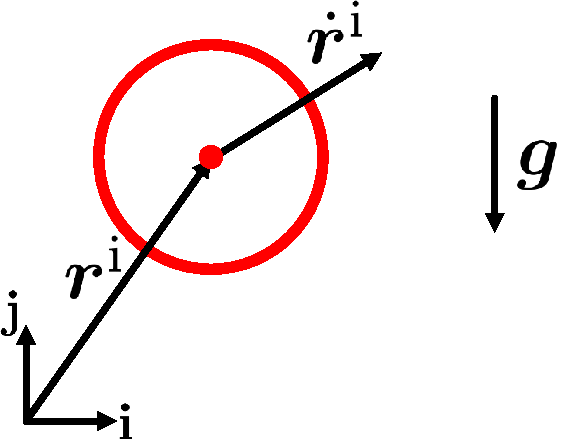
\includegraphics[width=0.3\textwidth]{images/falling_sphere/illustration.pdf}
	\label{fig:free_fall}
	\sourceMe
\end{figure}

Com isso, escrevendo \(\position = \explicitVectorCoordinates{\positionScalar}\), \(\velocity = \explicitVectorCoordinates{\velocityScalar}\) e \(\acceleration = \explicitVectorCoordinates{\accelerationScalar}\), é obtida a solução como apresentada na tabela \ref{table:free_fall_solution}.

\begin{table}[h]
	\caption{Solução do problema do lançamento oblíquo.}
	\label{table:free_fall_solution}

	\begin{equation*}
		\arraycolsep=1.5\arraycolsep
		\def\arraystretch{1.5}
		\begin{array}{lcc}
	\hline
		& \text{Direção } \xAxis 
		& \text{Direção } \yAxis \\
	\text{Posição} 
		& \positionx = \initial{\positionx} + \initial{\velocityx}\cdot \Dt
		& \positiony = \initial{\positiony} + \initial{\velocityy}\cdot \Dt - \dfrac{\gravityScalar\Dt^2}{2} \\
	\text{Velocidade} 
		& \velocityx = \initial{\velocityx}
		& \velocityy = \initial{\velocityy} - \gravityScalar\cdot \Dt \\
	\text{Aceleração} 
		& \accelerationx = 0
		& \accelerationy = - \gravityScalar \\
	\hline	
		\end{array}
	\end{equation*}
	\sourceMe
\end{table}

Embora seja conceitualmente simples e de fácil resolução, o problema do lançamento oblíquo permite:
\begin{itemize}
\item A validação numérica da implementação do algoritmo de Gear em simulações sem colisões, mas com a atuação de forças de campo. Em cada instante, as coordenadas da partícula são previstas e, em seguida, corrigidas a partir do valor da força da gravidade. A proximidade da resposta numericamente calculada com a solução analítica evidencia o bom funcionamento do algoritmo.
\item A obtenção da evolução do erro com o tempo de simulação. Não só existe um erro associado ao método como esse erro se acumula com o tempo.
\end{itemize}

A fim de se compararem os resultados numéricos com a solução analítica, foram arbitrados aos parâmetros do problema os valores dispostos na tabela \ref{tab:free_fall_case_parameters}.

\begin{table}[h]
\centering
\caption{Parâmetros para o problema de lançamento oblíquo.}
\label{tab:free_fall_case_parameters}
\begin{parametersdesc}
	\item{Gravidade}{\gravityScalar = 9,81}{\si[per-mode=symbol]{\metre\per\square\second}}
	\arrayrulecolor[gray]{0.8}\hline
	\item{Massa da partícula}{\mass = 1}{\si\kilogram}
	\item{Raio da partícula}{\radius = 3}{\si\centi\metre}
	\item{Posição inicial}{\explicitVector{\initial{\positionx}}{\initial{\positiony}}{\initial{\positionz}} = \explicitNumericVector{0}{0}{0}}{\si{\metre}}
	\item{Velocidade inicial}{\explicitVector{\initial{\velocityx}}{\initial{\velocityy}}{\initial{\velocityz}} = \explicitNumericVector{20}{10}{0}}{\si[per-mode=symbol]{\metre\per\second}}
	\item{Aceleração inicial}{\explicitVector{\initial{\accelerationx}}{\initial{\accelerationy}}{\initial{\accelerationz}} = \explicitNumericVector{0}{-9,81}{0}}{\si[per-mode=symbol]{\metre\per\square\second}}
	\arrayrulecolor[gray]{0.8}\hline
	\item{Instante final}{\finalInstant = 3}{\si\second} 
	\item{Passo de tempo}{\Dt = 10^{-3}}{\si\second}
	\item{Ordem de extrapolação}{\taylorOrder = 7}{\emptyUnit}
	\arrayrulecolor{black}
\end{parametersdesc}
\sourceMe 
\end{table}

Muito embora se trate de um problema bidimensional sem rotação, o simulador utiliza a formulação tridimensional e considera a evolução da velocidade angular da partícula.

\begin{figure}[htb!]
	\caption{Solução para a altura da partícula no problema de lançamento oblíquo\protect\footnotemark.}
	% \vspace{-0.5cm}
	\centering
		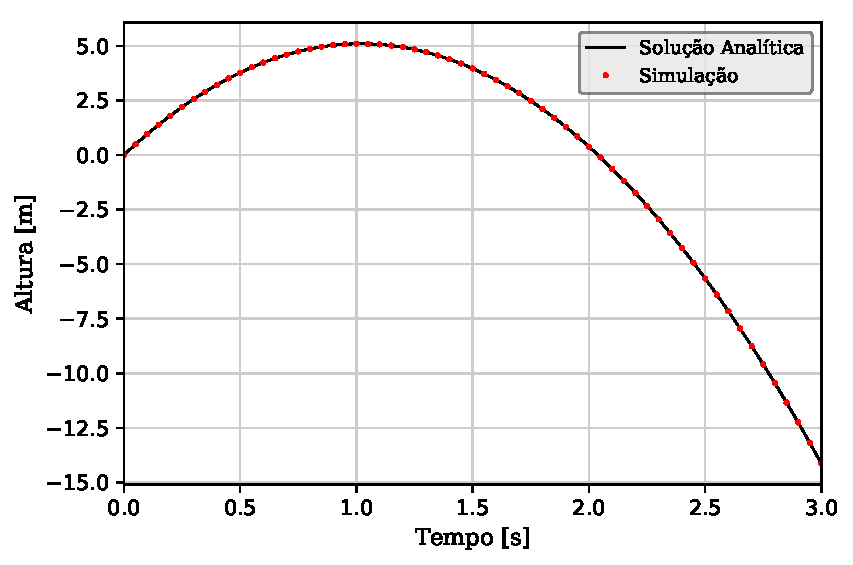
\includegraphics[scale=1]{images/falling_sphere/correct_initial_acceleration/y_position.pdf}
		% 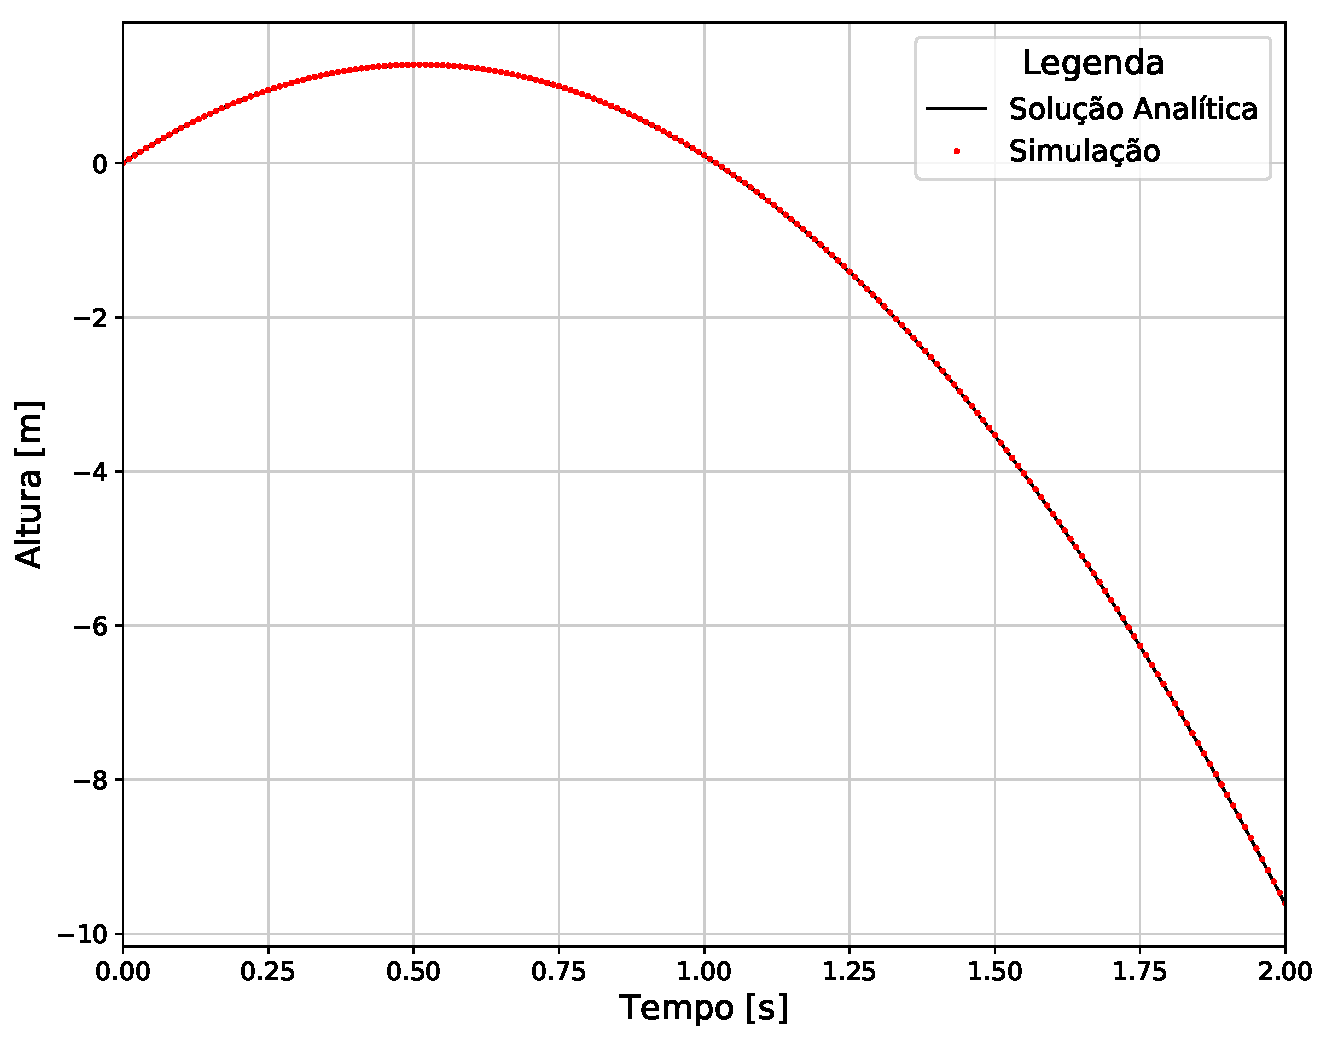
\includegraphics[width=\normalresultsfigwidth]{images/falling_sphere/y_position.pdf}
	% {\centerline{\includegraphics[scale=#2]{#1}}}
	% \vspace{-0.2cm}
	\label{fig:falling_sphere_y_position}
	\sourceMe
	% \vspace{-1cm}
\end{figure}

\footnotetext{Para melhor visualização dos resultados, é apresentado apenas um ponto a cada dez passos de tempo.}

\begin{figure}[htb!]
	\caption[Solução do problema de lançamento oblíquo para a posição horizontal, a velocidade horizontal, a velocidade vertical e a aceleração vertical da partícula]{Solução do problema de lançamento oblíquo para (\subref{subfig:x_position}) a posição horizontal, (\subref{subfig:x_velocity}) a velocidade horizontal, (\subref{subfig:y_velocity}) a velocidade vertical e (\subref{subfig:y_acceleration}) a aceleração vertical da partícula}
	% \vspace{-0.5cm}
	\centering
	\captionsetup[subfloat]{labelfont=bf}
	\subfloat{
		\centering
		\begin{subfigure}[t]{\smallresultsfigwidth}
			\centering
			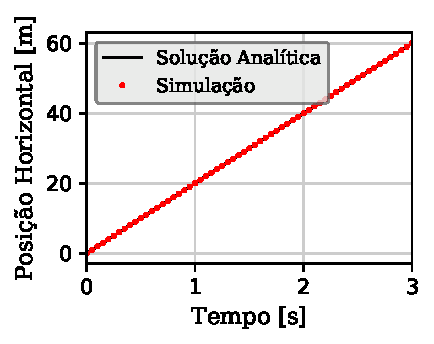
\includegraphics[scale=1]{images/falling_sphere/correct_initial_acceleration/x_position.pdf}
			\caption{}
			\label{subfig:x_position}
		\end{subfigure}
		\begin{subfigure}[t]{\smallresultsfigwidth}
			\centering
			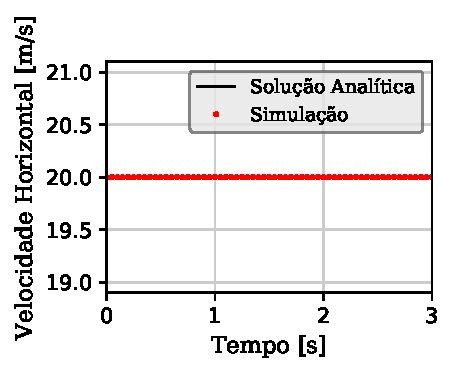
\includegraphics[scale=1]{images/falling_sphere/correct_initial_acceleration/x_velocity.pdf}
			\caption{}
			\label{subfig:x_velocity}
		\end{subfigure}
		\begin{subfigure}[t]{\smallresultsfigwidth}
			\centering
			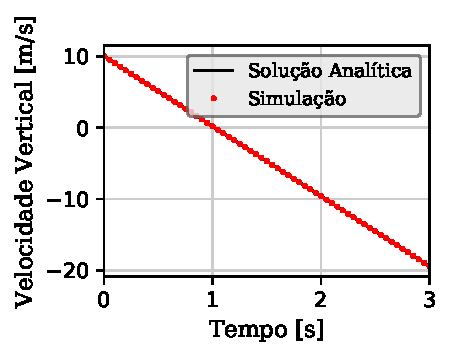
\includegraphics[scale=1]{images/falling_sphere/correct_initial_acceleration/y_velocity.pdf}
			\caption{}
			\label{subfig:y_velocity}
		\end{subfigure}
		\begin{subfigure}[t]{\smallresultsfigwidth}
			\centering
			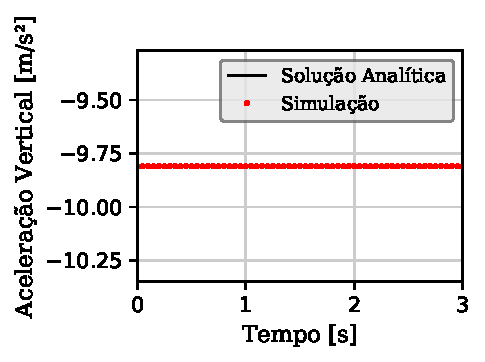
\includegraphics[scale=1]{images/falling_sphere/correct_initial_acceleration/y_acceleration.pdf}
			\caption{}
			\label{subfig:y_acceleration}
		\end{subfigure}
	}
	% \vspace{-0.2cm}
	\label{fig:falling_sphere_other}
	\sourceMe
	% \vspace{-1cm}
\end{figure}

Com esses parâmetros, foi calculada a trajetória da partícula através do simulador e da solução analítica. Na \cref{fig:falling_sphere_y_position} estão expostas as soluções para a altura da partícula. Observa-se nessa figura que os resultados obtidos pelo simulador se aproximam bastante da solução analítica das equações.

Outras variáveis, como a posição horizontal, as velocidades horizontal e vertical e a aceleração vertical estão apresentadas na \cref{fig:falling_sphere_other}.

\begin{figure}[htb!]
	\caption[Erro da simulação com relação à solução numérica para a posição e da partícula do problema do lançamento oblíquo]{Erro da simulação com relação à solução numérica para (\subref{subfig:position_error}) a posição e (\subref{subfig:velocity_error}) da partícula do problema do lançamento oblíquo}
	% \vspace{-0.5cm}
	\centering
	\captionsetup[subfloat]{labelfont=bf}
	\subfloat{
		\centering
		\begin{subfigure}[t]{\smallresultsfigwidth}
			\centering
			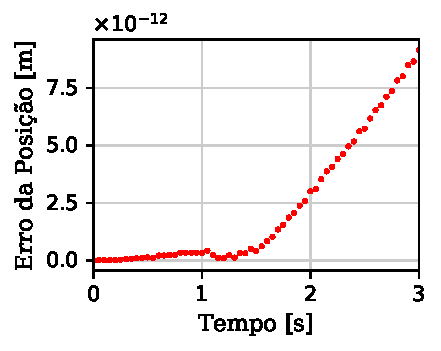
\includegraphics[scale=1]{images/falling_sphere/correct_initial_acceleration/position_error.pdf}
			\caption{}
			\label{subfig:position_error}
		\end{subfigure}
		\begin{subfigure}[t]{\smallresultsfigwidth}
			\centering
			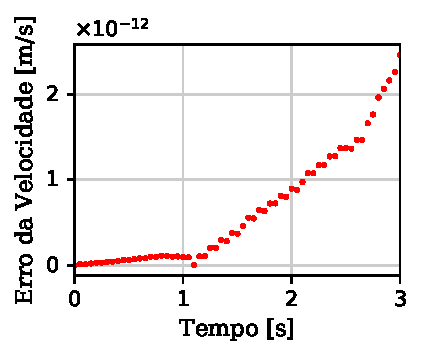
\includegraphics[scale=1]{images/falling_sphere/correct_initial_acceleration/velocity_error.pdf}
			\caption{}
			\label{subfig:velocity_error}
		\end{subfigure}
	}
	% \vspace{-0.2cm}
	\label{fig:falling_sphere_error}
	\sourceMe
	% \vspace{-1cm}
\end{figure}

Por sua vez, o erro da posição e o erro da velocidade, como funções do tempo, são apresentados na \cref{fig:falling_sphere_error}. Esses erros são calculados de acordo com a equação \eqref{eq:vector_error}. Observa-se nessa \namecref{fig:falling_sphere_error} que o erro da posição se mantém inferior a \SI{0,01}{\nano\meter} durante toda a simulação, evidenciando a exatidão do método. Além disso, é possível notar que o erro se acumula com o avanço da simulação.

O arquivo em formato \JSON{} utilizado para essa simulação é apresentado no \cref{app:code_listings}.

\section{Esfera Quicando}

Como extensão do problema de queda livre, o problema da esfera quicando inclui, além da gravidade, a colisão entre uma esfera e uma parede plana. Supõe-se uma partícula \(\particle\) esférica de raio \(\radius\) e massa \(\mass\) que, no instante inicial \(\initialInstant=0\), é liberada no espaço, em repouso, na posição \(\initial{\position} = \explicitVector{0}{\initial{\positiony}}{0}\).

A partícula está sujeita a um campo gravitacional constante cuja aceleração da gravidade é \(\gravity = -\gravityScalar\cdot\yUnit\) com \(\gravityScalar>0\). Nessa situação, a componente \(\positiony\) denota a altura da partícula.

Além disso, considera-se um elemento \(\element\) identificado com o plano \(\xAxis\zAxis\) representando o chão. Sendo um plano fixo, esse elemento é completamente determinado ao se fornecerem um ponto e um versor normal a ele. Para o plano \(\xAxis\zAxis\), podem ser adotados a origem \(\originPoint\) do sistema como ponto pertencente ao plano e o versor normal \(\planeNormalVersor = \explicitVector{0}{1}{0}\).

Essa configuração pode ser representada como na figura \ref{fig:bouncing_sphere}.

\begin{figure}[h]
	\caption{O problema da esfera quicando.}
	% \vspace{-0.5cm}
	\centering
		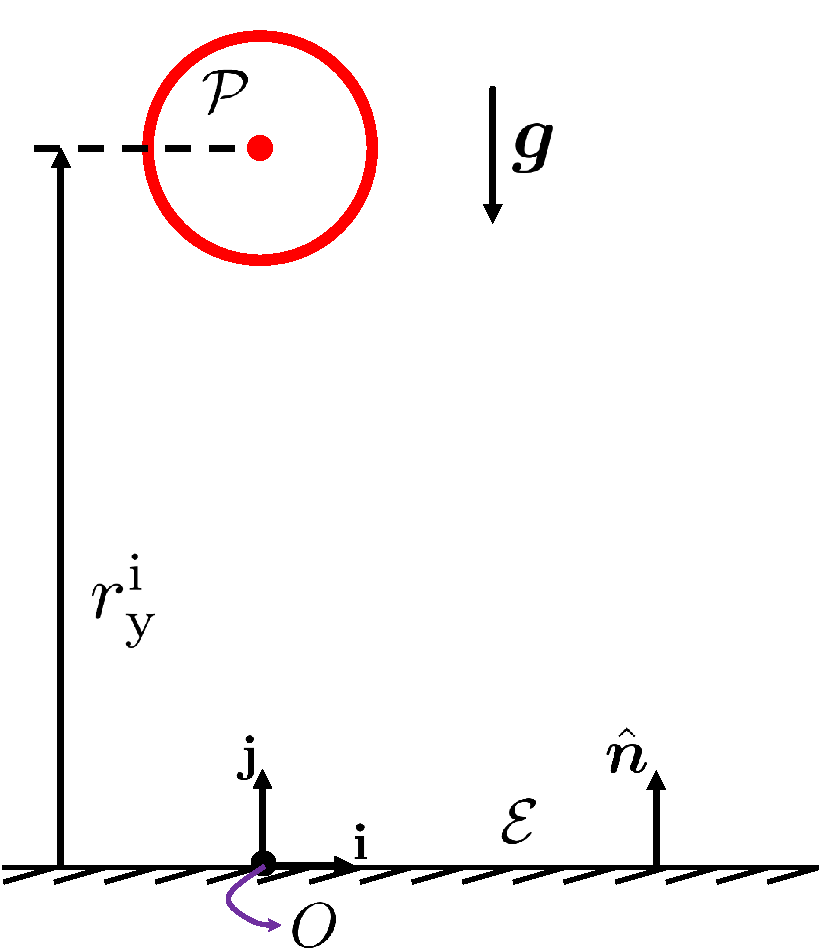
\includegraphics[width=0.35\textwidth]{images/bouncing_sphere/illustration.pdf}
	\label{fig:bouncing_sphere}
	\sourceMe
\end{figure}

Além de servir como mais um caso para a validação do código, o problema da esfera quicando possibilita a comparação entre o coeficiente de restituição calculado a partir dos resultados da simulação e o coeficiente calculado analiticamente a partir do modelo de força escolhido.

A configuração do problema implica que a velocidade da esfera relativa ao plano é a sua própria velocidade vertical, já que o plano não se movimenta. Como consequência das equações \eqref{eq:antisymmetry_relative_velocity} e \eqref{eq:sphere_plane_relative_velocity}, essa velocidade é a própria velocidade da partícula.

Com isso, sendo \(\coefficientOfRestitution\) o coeficiente de restituição associado ao modelo de força de colisão escolhido, é possível mostrar que
\begin{equation} \label{eq:coefficient_of_restitution_with_gravity}
	\coefficientOfRestitution = - \dfrac{\afterCollision{\yComponent{\velocityScalar}} + \gravityScalar\cdot\collisionDuration}{\beforeCollision{\yComponent{\velocityScalar}}},
\end{equation}
sendo \(\afterCollision{\yComponent{\velocityScalar}}\) a velocidade da partícula \(\particle\) após a colisão com o chão, e \(\collisionDuration\), o tempo em que os corpos permanecem em contato. O termo \(\gravityScalar\cdot\collisionDuration\) é uma compensação feita pelo fato de que, no problema em questão, a gravidade contribui para a variação da velocidade das partículas, o que não é considerado no cálculo analítico do coeficiente de restituição.

Para a solução desse problema, foram escolhidos dois casos: um dissipativo (\cref{sec:results:bouncing_sphere:dissipative_case}), em que os elementos da simulação possuem constante de amortecimento não nula, e um conservativo (\cref{sec:results:bouncing_sphere:conservative}), em que essa constante é zero.

\subsection{Caso Dissipativo} \label{sec:results:bouncing_sphere:dissipative_case}

Para o estudo do problema da esfera quicando, foram considerados os parâmetros de simulação expostos na tabela \ref{tab:bouncing_sphere:dissipative_case:parameters}. O modelo de interação considerado é o modelo do amortecimento linear corrigido, cuja expressão para a força é dada pela \cref{eq:corrected_linear_dashpot:normal_force}, enquanto o coeficiente de restituição é calculado pela \cref{eq:corrected_linear_dashpot:coefficient_of_restitution}.

\begin{table}[h]
\centering
\caption{Parâmetros para o caso dissipativo do problema da esfera quicando.}
\label{tab:bouncing_sphere:dissipative_case:parameters}
\begin{parametersdesc}
	\item{Modelo de força normal}{\text{Amortecedor linear corrigido}}{\emptyUnit}
	\item{Gravidade}{\gravityScalar = 9,81}{\si[per-mode=symbol]{\metre\per\square\second}}
	\arrayrulecolor[gray]{0.8}\hline
	\item{Massa da partícula}{\ind{\mass}{\particle} = 1}{\si\kilogram}
	\item{Raio da partícula}{\ind{\radius}{\particle} = 3}{\si\centi\metre}
	\item{Constante elástica da partícula}{\ind{\elasticModulus}{\particle} = 1}{\si[per-mode=symbol]{\giga\pascal}}
	\item{Constante de amortecimento da partícula}{\ind{\normalDampingConstant}{\particle} = \SI{5000}{}}{\si[per-mode=symbol]{\newton\second\per\meter}}
	\arrayrulecolor[gray]{0.8}\hline
	\item{Altura inicial da partícula}{\initial{\positiony} = 1}{\si{\metre}}
	\item{Velocidade inicial da partícula}{\explicitVector{\initial{\velocityx}}{\initial{\velocityy}}{\initial{\velocityz}} = \explicitVector{0}{0}{0}}{\si[per-mode=symbol]{\metre\per\second}}
	\item{Aceleração inicial da partícula}{\explicitVector{\initial{\accelerationx}}{\initial{\accelerationy}}{\initial{\accelerationz}} = \explicitVector{0}{0}{0}}{\si[per-mode=symbol]{\metre\per\square\second}}
	\arrayrulecolor[gray]{0.8}\hline
	\item{Ponto da parede}{\ind{\planeOrigin}{\element} = \explicitVector{0}{0}{0}}{\si\meter}
	\item{Versor normal à parede}{\ind{\planeNormalVersor}{\element} = \explicitVector{0}{1}{0}}{\si\metre}
	\item{Constante elástica da parede}{\ind{\elasticModulus}{\element} = 1}{\si[per-mode=symbol]{\giga\pascal}}
	\item{Constante de amortecimento da parede}{\ind{\normalDampingConstant}{\element} = \SI{5000}{}}{\si[per-mode=symbol]{\newton\second\per\meter}}
	\arrayrulecolor[gray]{0.8}\hline
	\item{Instante final}{\finalInstant = 10}{\si\second} 
	\item{Passo de tempo}{\Dt = 10^{-5}}{\si\second}
	\item{Ordem de extrapolação}{\taylorOrder = 7}{\emptyUnit}
	\arrayrulecolor{black}
\end{parametersdesc}
\sourceMe 
\end{table}

\begin{figure}[htb!]
	\caption{Solução para a altura da partícula no caso dissipativo do problema da esfera quicando.}
	\centering
		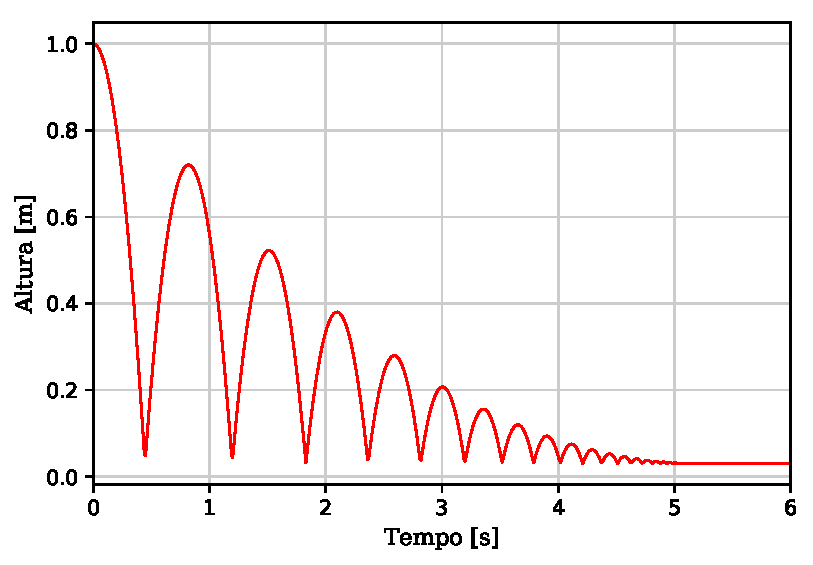
\includegraphics[scale=1]{images/bouncing_sphere/dissipative/y_position.pdf}
	\label{fig:bouncing_sphere_y_position}
	\sourceMe
\end{figure}

A partir desses parâmetros, uma simulação foi executada, resultando na altura da partícula em função do tempo como exposta na \cref{fig:bouncing_sphere_y_position}.

\begin{figure}[h]
	\caption[Energia cinética e energia mecânica da partícula no caso dissipativo do problema da esfera quicando.]{Energia cinética (\subref{subfig:bouncing_sphere:kinetic_energy}) e energia mecânica (\subref{subfig:bouncing_sphere:mechanical_energy}) da partícula no caso dissipativo do problema da esfera quicando.}
	% \vspace{-0.5cm}
	\centering
	\captionsetup[subfloat]{labelfont=bf}
	\subfloat{
		\centering
		\begin{subfigure}[t]{\smallresultsfigwidth}
			\centering
			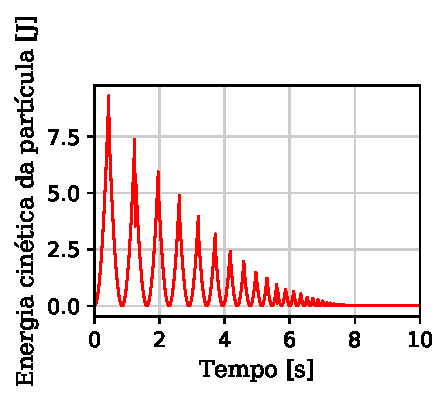
\includegraphics[scale=1]{images/bouncing_sphere/dissipative/kinetic_energy.pdf}
			\caption{}
			\label{subfig:bouncing_sphere:kinetic_energy}
		\end{subfigure}
		\begin{subfigure}[t]{\smallresultsfigwidth}
			\centering
			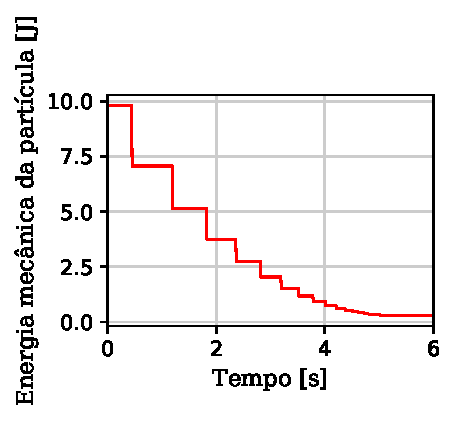
\includegraphics[scale=1]{images/bouncing_sphere/dissipative/mechanical_energy.pdf}
			\caption{}
			\label{subfig:bouncing_sphere:mechanical_energy}
		\end{subfigure}
	}
	\sourceMe
	\label{fig:bouncing_sphere_energy}
	% \vspace{-1cm}
\end{figure}

Uma análise importante a se fazer nesse problema é a da energia. A energia cinética e a energia mecânica resultantes da simulação, calculadas de acordo com as \cref{eq:kineticEnergy,eq:mechanicalEnergy}, são apresentadas na \cref{fig:bouncing_sphere_energy}. Observa-se nos gráficos que a partícula experiencia uma queda em sua sua energia mecânica após as colisões com o chão, sendo que a energia cinética anula-se aproximadamente após \SI{5}{\second} de simulação.

\begin{figure}[h]
	\caption{Coeficiente de restituição resultante da colisão dissipativa do problema da esfera quicando.}
	\centering
		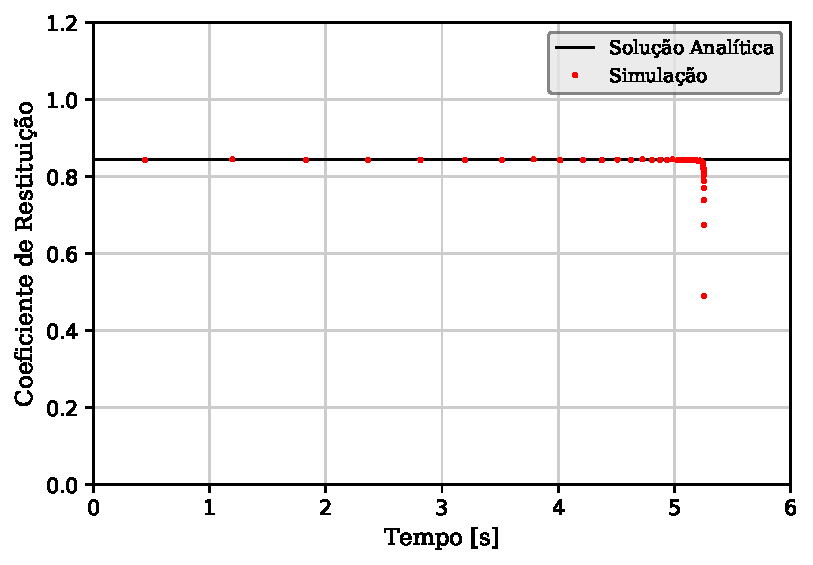
\includegraphics[scale=1]{images/bouncing_sphere/dissipative/coefficient_of_restitution.pdf}
		% 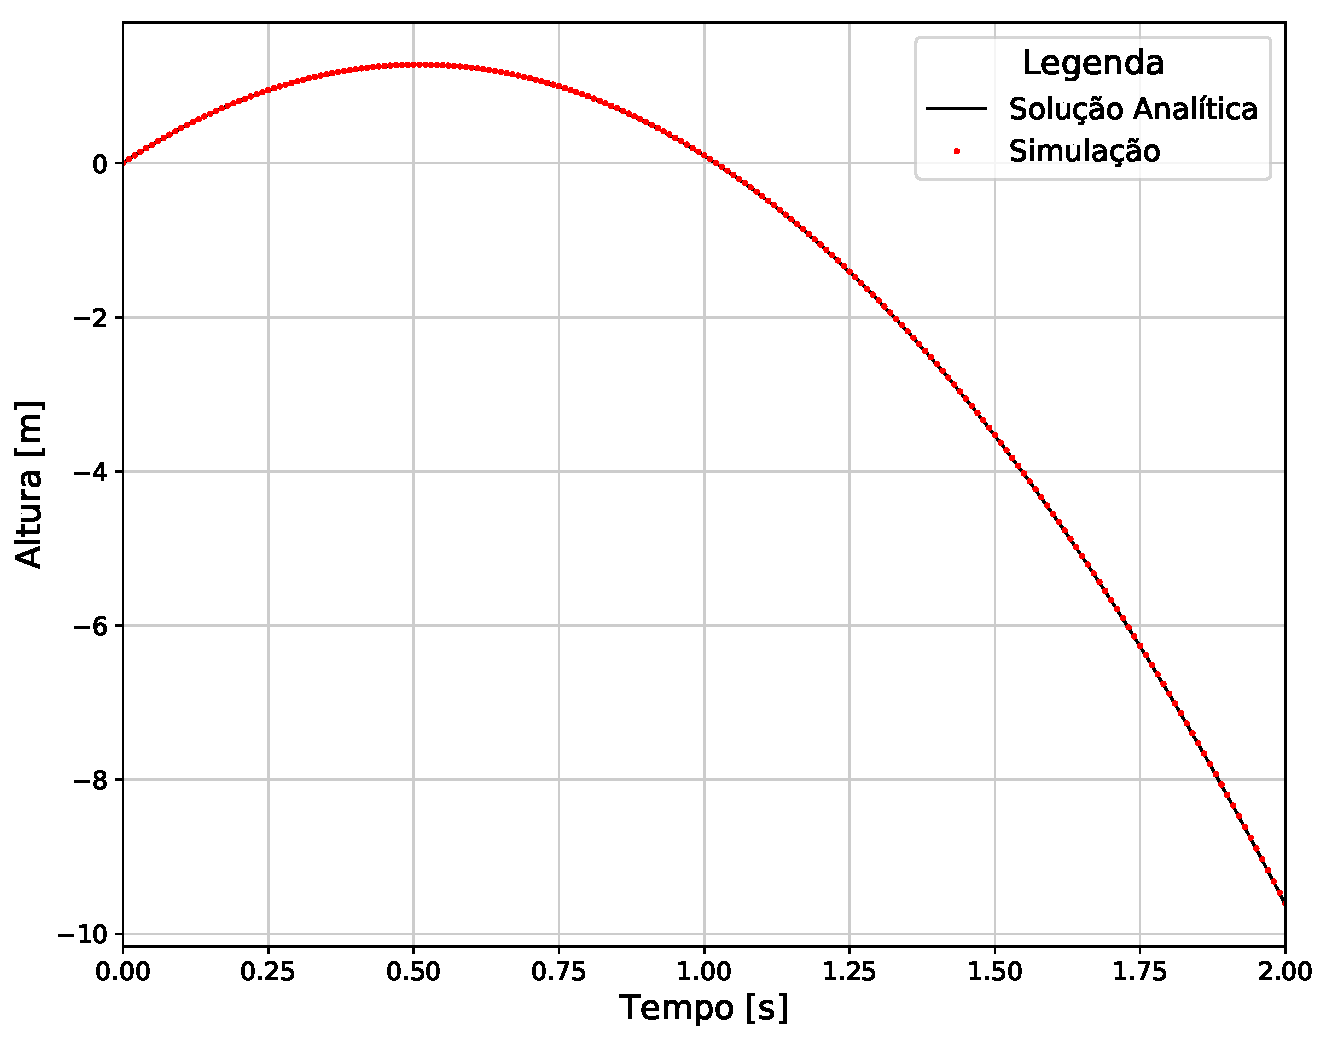
\includegraphics[width=\normalresultsfigwidth]{images/falling_sphere/y_position.pdf}
	% {\centerline{\includegraphics[scale=#2]{#1}}}
	\label{fig:bouncing_sphere:dissipative:coefficient_of_restitution}
	\sourceMe
\end{figure}

Além da energia, o coeficiente de restituição resultante da colisão também pode ser estudado. Na \cref{fig:bouncing_sphere:dissipative:coefficient_of_restitution}, estão representados o coeficiente calculado numericamente através da \cref{eq:coefficient_of_restitution_with_gravity} e o coeficiente analítico dado pela expressão \eqref{eq:corrected_linear_dashpot:coefficient_of_restitution}. Observa-se uma boa concordância entre os resultados até aproximadamente \SI{5}{\second} de simulação. A divergência que ocorre após esse instante explica-se pelo fato de que a partícula entra em repouso sobre o chão.

\subsection{Caso Conservativo} \label{sec:results:bouncing_sphere:conservative}

O caso dissipativo, como exposto na \cref{sec:results:bouncing_sphere:dissipative_case}, apresenta uma dissipação da energia causada pelo amortecimento do modelo de colisão adotado. Nesta \namecref{sec:results:bouncing_sphere:conservative}, considera-se o caso conservativo.

\begin{table}[h]
\centering
\caption{Parâmetros para o caso dissipativo do problema da esfera quicando.}
\label{tab:bouncing_sphere:conservative:parameters}
\begin{parametersdesc}
	\item{Constante de amortecimento da partícula}{\ind{\normalDampingConstant}{\particle} = 0}{\si[per-mode=symbol]{\newton\second\per\meter}}
	\item{Constante de amortecimento da parede}{\ind{\normalDampingConstant}{\element} = 0}{\si[per-mode=symbol]{\newton\second\per\meter}}
	\item{Demais parâmetros}{\text{\Cref{tab:bouncing_sphere:dissipative_case:parameters}}}{}
\end{parametersdesc}
\sourceMe 
\end{table}
\alert{Essa tabela ficou feia!}

\alert{Tirar o gráfico da energia e dizer que ela se conserva exceto nos choques}

\begin{figure}[htb!]
	\caption[Altura e energia mecânica da partícula e coeficiente de restituição no caso conservativo do problema da esfera quicando.]{Altura (\subref{subfig:bouncing_sphere:conservative:height}) e energia mecânica (\subref{subfig:bouncing_sphere:conservative:mechanical_energy}) da partícula e coeficiente de restituição (\subref{subfig:bouncing_sphere:conservative:coefficient_of_restitution}) no caso conservativo do problema da esfera quicando.}
	\centering
	\captionsetup[subfloat]{labelfont=bf}
	\subfloat{
		\centering
		\begin{subfigure}[t]{\smallresultsfigwidth}
			\centering
			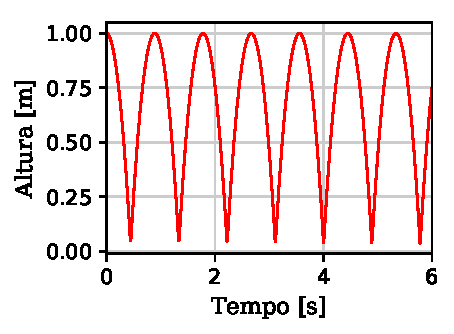
\includegraphics[scale=1]{images/bouncing_sphere/conservative/small_y_position.pdf}
			\caption{}
			\label{subfig:bouncing_sphere:conservative:height}
		\end{subfigure}
		\begin{subfigure}[t]{\smallresultsfigwidth}
			\centering
			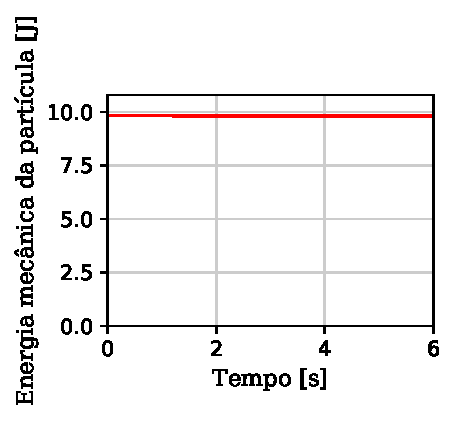
\includegraphics[scale=1]{images/bouncing_sphere/conservative/mechanical_energy.pdf}
			\caption{}
			\label{subfig:bouncing_sphere:conservative:mechanical_energy}
		\end{subfigure}
		\begin{subfigure}[t]{\smallresultsfigwidth}
			\centering
			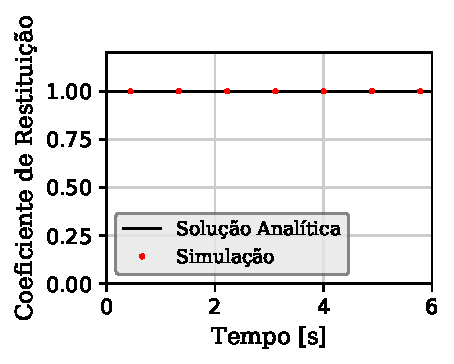
\includegraphics[scale=1]{images/bouncing_sphere/conservative/small_coefficient_of_restitution.pdf}
			\caption{}
			\label{subfig:bouncing_sphere:conservative:coefficient_of_restitution}
		\end{subfigure}
	}
	\sourceMe
	\label{fig:bouncing_sphere:conservative}
\end{figure}

Para essa simulação, foram utilizados parâmetros idênticos aos indicados na \cref{tab:bouncing_sphere:dissipative_case:parameters}, à exceção das constantes de amortecimento. Essas constantes são responsáveis pela dissipação da energia, e, para o caso conservativo, devem tomar valor nulo, como indicado na \cref{tab:bouncing_sphere:conservative:parameters}.

\begin{table}[h]
\centering
\caption{Energia mecânica e coeficiente de restituição resultantes do caso conservativo do problema da esfera quicando.}
\label{tab:bouncing_sphere:conservative:energy_and_coefficient_of_restitution}
\begin{parametersdesc}
	\item{Energia mecânica inicial}{\initial{\mechanicalEnergy} = \SI{9,81}{\joule}}{}
	\item{Energia mecânica final}{\final{\mechanicalEnergy} = \SI{9,80644775955}{\joule}}{}
	\item{Variação da energia mecânica}{\Delta \mechanicalEnergy = \initial{\mechanicalEnergy} - \final{\mechanicalEnergy} = \SI{3,552}{\milli\joule}}{}
	\item{Percentual de energia dissipada}{\bigslant{\Delta\mechanicalEnergy}{\initial{\mechanicalEnergy}} = \SI{0,036}{\percent}}{}
	\item{Coeficiente de restituição analítico}{\coefficientOfRestitution = 1}{}
	\item{Erro máximo do coeficiente de restituição}{\maximumErrorOf{\coefficientOfRestitution} = 2\cdot 10^{-4}}{}
	\item{Erro máximo percentual do coeficiente de restituição}{\bigslant{\maximumErrorOf{\coefficientOfRestitution}}{\coefficientOfRestitution} = \SI{0,02}{\percent}}{}
\end{parametersdesc}
\sourceMe 
\end{table}

Nessa situação, os resultados obtidos pela simulação para a altura e a energia mecânica da partícula e para o coeficiente de restituição são obtidos como na \cref{fig:bouncing_sphere:conservative}. Observa-se nessa \namecref{fig:bouncing_sphere:conservative} que a energia se conserva, sendo constante com exceção dos instantes de colisão, em que a energia mecânica se transforma em energia puramente elástica. De fato, a diferença observada entre a energia mecânica inicial \(\initial{\mechanical{\energy}}\) e a final \(\final{\mechanical{\energy}}\) foi da ordem de \(10^{-3}\si{\joule}\), o que representa \SI{0,036}{\percent} da energia inicial. Por sua vez, o coeficiente de restituição manteve-se bastante próximo de \(1\), o que corresponde ao resultado analítico, com erro máximo de \SI{0,02}{\percent}. Esses resultados estão expostos na \cref{tab:bouncing_sphere:conservative:energy_and_coefficient_of_restitution}.


\section{Colisão entre Esferas} \label{sec:results:colliding_spheres}

A questão central dos métodos de elementos discretos é a interação entre partículas, situação em que existem duas ou mais equações de movimento a serem resolvidas simultaneamente. Nesta \namecref{sec:results:colliding_spheres}, é apresentado o problema da colisão entre duas esferas.

\begin{figure}[h]
	\caption{O problema da colisão entre esferas.}
	\centering
		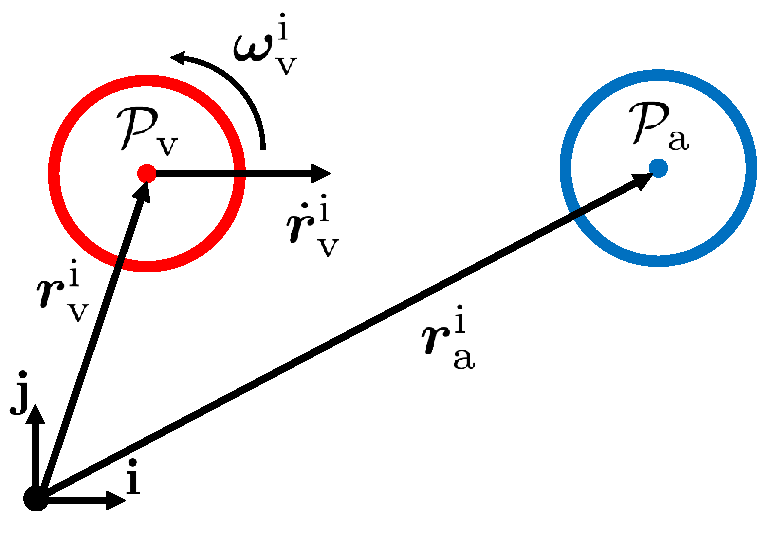
\includegraphics[width=0.45\textwidth]{images/colliding_spheres/illustration.pdf}
	\label{fig:colliding_spheres}
	\sourceMe
\end{figure}

Consideram-se duas partículas esféricas: a partícula vermelha \(\redParticle\) e a azul \(\blueParticle\). A partícula azul encontra-se em repouso na posição \(\initial{\bluePosition}\). A partícula vermelha encontra-se inicialmente na posição \(\initial{\redPosition}\) e avança, com uma velocidade linear \(\initial{\redVelocity}\) e uma velocidade angular \(\initial{\redAngularVelocity} = \initial{\redAngularVelocityScalar}\cdot\zUnit\), na direção de \(\blueParticle\). As partículas colidem, e ocorre transferência de movimento da partícula vermelha para a azul. Essa situação é representada na \cref{fig:colliding_spheres}.

Nesse problema, não é considerada a ação da gravidade, o que permite a análise simples das quantidades de movimento linear a angular. Como no problema da esfera quicando, são consideradas duas situações: o caso conservativo e o caso dissipativo. Devido à natureza das forças tangenciais apresentadas na \cref{sec:collision_force_models}, simulações com rotações são intrinsecamente dissipativas, e por isso esse caso só é considerado na \cref{sec:colliding_spheres:dissipative}.

\subsection{Caso Conservativo}

Para a simulação com conservação da energia, foram escolhidos os parâmetros expostos na \cref{tab:colliding_spheres:conservative:parameters}. Novamente, foi escolhido o modelo de força normal de amortecimento linear pela facilidade de se examinar o coeficiente de restituição resultante.

\begin{table}[h]
\centering
\caption{Parâmetros para o caso conservativo do problema da esfera quicando.}
\label{tab:colliding_spheres:conservative:parameters}
\begin{parametersdesc}
	\item{Modelo de força normal}{\text{Amortecedor linear corrigido}}{\emptyUnit}
	\arrayrulecolor[gray]{0.8}\hline
	\item{Massa da partícula vermelha}{\redMass = 1}{\si\kilogram}
	\item{Raio da partícula vermelha}{\redRadius = 3}{\si\centi\metre}
	\item{Constante elástica da partícula vermelha}{\redElasticModulus = 1}{\si[per-mode=symbol]{\giga\pascal}}
	\item{Constante de amortecimento normal da partícula vermelha}{\redNormalDampingConstant = 0}{\si[per-mode=symbol]{\newton\second\per\meter}}
	\arrayrulecolor[gray]{0.8}\hline
	\item{Posição inicial da partícula vermelha}{\initial{\redPosition} = \explicitVector{0}{0}{0}}{\si{\metre}}
	\item{Velocidade inicial da partícula vermelha}{\initial{\redVelocity} = \explicitVector{10}{0}{0}}{\si[per-mode=symbol]{\metre\per\second}}
	\item{Aceleração inicial da partícula vermelha}{\initial{\redAcceleration} = \explicitVector{0}{0}{0}}{\si[per-mode=symbol]{\metre\per\square\second}}
	\arrayrulecolor[gray]{0.8}\hline
	\item{Massa da partícula azul}{\blueMass = 1}{\si\kilogram}
	\item{Raio da partícula azul}{\blueRadius = 3}{\si\centi\metre}
	\item{Constante elástica da partícula azul}{\blueElasticModulus = 1}{\si[per-mode=symbol]{\giga\pascal}}
	\item{Constante de amortecimento normal da partícula azul}{\blueNormalDampingConstant = 0}{\si[per-mode=symbol]{\newton\second\per\meter}}
	\arrayrulecolor[gray]{0.8}\hline
	\item{Posição inicial da partícula azul}{\initial{\bluePosition} = \explicitVector{62}{0}{0}}{\si{\milli\metre}}
	\item{Velocidade inicial da partícula azul}{\initial{\blueVelocity} = \explicitVector{0}{0}{0}}{\si[per-mode=symbol]{\metre\per\second}}
	\item{Aceleração inicial da partícula azul}{\initial{\blueAcceleration} = \explicitVector{0}{0}{0}}{\si[per-mode=symbol]{\metre\per\square\second}}
	\arrayrulecolor[gray]{0.8}\hline
	\item{Instante final}{\finalInstant = 1}{\si\milli\second} 
	\item{Passo de tempo}{\Dt = 10^{-8}}{\si\second}
	\item{Ordem de extrapolação}{\taylorOrder = 7}{\emptyUnit}
	\arrayrulecolor{black}
\end{parametersdesc}
\sourceMe 
\end{table}

Com esses parâmetros, foi executada a simulação conservativa. A posição e a velocidade das partículas são apresentadas na \cref{fig:colliding_spheres:conservative:position_and_velocity}.

\begin{figure}[htb!]
	\caption[Solução para a posição horizontal e a velocidade horizontal das partículas colidentes na simulação conservativa.]{Solução para a posição horizontal (\subref{subfig:colliding_spheres:conservative:x_position}) e a velocidade horizontal (\subref{subfig:colliding_spheres:conservative:x_velocity}) das partículas colidentes na simulação conservativa.}
	\centering
	\captionsetup[subfloat]{labelfont=bf}
	\subfloat{
		\centering
		\begin{subfigure}[t]{\smallresultsfigwidth}
			\centering
			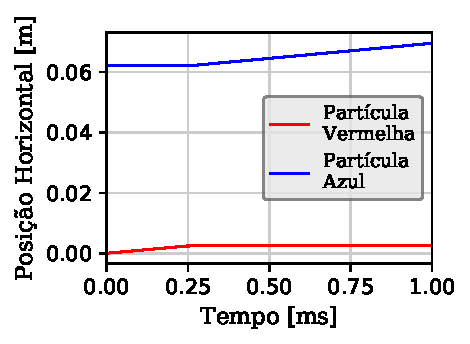
\includegraphics[scale=1]{images/colliding_spheres/conservative/Position-X_small.pdf}
			\caption{}
			\label{subfig:colliding_spheres:conservative:x_position}
		\end{subfigure}
		\begin{subfigure}[t]{\smallresultsfigwidth}
			\centering
			\includegraphics[scale=1]{images/colliding_spheres/conservative/Velocity-X_small.pdf}
			\caption{}
			\label{subfig:colliding_spheres:conservative:x_velocity}
		\end{subfigure}
	}
	\label{fig:colliding_spheres:conservative:position_and_velocity}
	\sourceMe
\end{figure}

Também é possível representarem-se a quantidade de movimento linear horizontal, a força de contato horizontal entre as partículas, a energia cinética e o coeficiente de restituição resultante do choque, como na \cref{fig:colliding_spheres:conservative:linear_momentum_force_kinetic_energy_and_coefficient_of_restitution}.

\begin{figure}[htb!]
	\caption[Curvas da quantidade de movimento linear, da força de contato horizontal, da energia cinética e do coeficiente de restituição do par de partículas colidentes na simulação conservativa.]{Curvas da quantidade de movimento linear (\subref{subfig:colliding_spheres:conservative:x_linear_momentum}), da força de contato horizontal (\subref{subfig:colliding_spheres:conservative:x_contact_force}), da energia cinética (\subref{subfig:colliding_spheres:conservative:kinetic_energy}) e do coeficiente de restituição (\subref{subfig:colliding_spheres:conservative:coefficient_of_restitution}) do par de partículas colidentes na simulação conservativa.}
	\centering
	\captionsetup[subfloat]{labelfont=bf}
	\subfloat{
		\centering
		\begin{subfigure}[t]{\smallresultsfigwidth}
			\centering
			\includegraphics[scale=1]{images/colliding_spheres/conservative/linearMomentum-X_small_total.pdf}
			\caption{}
			\label{subfig:colliding_spheres:conservative:x_linear_momentum}
		\end{subfigure}
		\begin{subfigure}[t]{\smallresultsfigwidth}
			\centering
			\includegraphics[scale=1]{images/colliding_spheres/conservative/contactForce-X_small.pdf}
			\caption{}
			\label{subfig:colliding_spheres:conservative:x_contact_force}
		\end{subfigure}
		\begin{subfigure}[t]{\smallresultsfigwidth}
			\centering
			\includegraphics[scale=1]{images/colliding_spheres/conservative/kineticEnergy_small_total.pdf}
			\caption{}
			\label{subfig:colliding_spheres:conservative:kinetic_energy}
		\end{subfigure}
		\begin{subfigure}[t]{\smallresultsfigwidth}
			\centering
			\includegraphics[scale=1]{images/colliding_spheres/conservative/coefficient_of_restitution_small.pdf}
			\caption{}
			\label{subfig:colliding_spheres:conservative:coefficient_of_restitution}
		\end{subfigure}
	}
	\label{fig:colliding_spheres:conservative:linear_momentum_force_kinetic_energy_and_coefficient_of_restitution}
	\sourceMe
\end{figure}

\begin{table}[h]
\centering
\caption{Coeficiente de restituição resultante do caso conservativo do problema das esferas colidentes.}
\label{tab:colliding_spheres:conservative:energy_and_coefficient_of_restitution}
\begin{parametersdesc}
	\item{Coeficiente de restituição analítico}{\coefficientOfRestitution = 1}{}
	\item{Erro máximo do coeficiente de restituição}{\maximumErrorOf{\coefficientOfRestitution} = 9\cdot 10^{-9}}{}
\end{parametersdesc}
\sourceMe 
\end{table}

Como pode ser observado, os resultados aproximam-se bastante do esperado. Por se tratar de uma colisão sem termos dissipativos, a partícula vermelha transfere todo o seu movimento à azul, entrando em repouso após a colisão. A \cref{subfig:colliding_spheres:conservative:coefficient_of_restitution} e a \cref{tab:colliding_spheres:conservative:energy_and_coefficient_of_restitution} indicam que o coeficiente de restituição numericamente calculado praticamente se iguala ao analítico com valor unitário, o que implica uma colisão perfeitamente elástica. Mais ainda, infere-se das \cref{subfig:colliding_spheres:conservative:x_linear_momentum,subfig:colliding_spheres:conservative:kinetic_energy} que ocorre a conservação da quantidade de movimento e a conservação da energia. Além disso, chama a atenção o fato de que parte da energia cinética é transformada em energia elástica durante o choque, e é restituída finda a colisão. Também é interessante notar que a força de colisão entre as partículas, indicada na \cref{subfig:colliding_spheres:conservative:x_contact_force}, ultrapassa os \SI{150}{\kilo\newton} em módulo.

\subsection{Caso Dissipativo} \label{sec:colliding_spheres:dissipative}

No caso dissipativo, são atribuídas às partículas constantes de amortecimento não nulas. A simulação dissipativa pode ser separada em dois casos: sem rotação e com rotação.

\subsubsection{Sem Rotação}

Para a simulação dissipativa sem rotação, consideram-se os parâmetros da \cref{tab:colliding_spheres:dissipative:parameters}. Os resultados desse caso podem ser compilados como na \cref{fig:colliding_spheres:dissipative:results}.

\begin{table}[h]
\centering
\caption{Parâmetros para o caso dissipativo do problema da colisão entre esferas.}
\label{tab:colliding_spheres:dissipative:parameters}
\begin{parametersdesc}
	\item{Constante de amortecimento da partícula vermelha}{\redNormalDampingConstant = 10000}{\si[per-mode=symbol]{\newton\second\per\meter}}
	\item{Constante de amortecimento da partícula azul}{\blueNormalDampingConstant = 10000}{\si[per-mode=symbol]{\newton\second\per\meter}}
	\item{Demais parâmetros}{\text{\Cref{tab:colliding_spheres:conservative:parameters}}}{}
\end{parametersdesc}
\sourceMe 
\end{table}

\begin{figure}[htb!]
	\caption[Solução da posição, da velocidade, da quantidade de movimento linear, da força de contato horizontal, da energia cinética e do coeficiente de restituição do par de partículas colidentes na simulação dissipativa sem rotação.]{Solução da posição (\subref{subfig:colliding_spheres:dissipative:x_position}), da velocidade (\subref{subfig:colliding_spheres:dissipative:x_velocity}), da quantidade de movimento linear (\subref{subfig:colliding_spheres:dissipative:x_linear_momentum}), da força de contato horizontal (\subref{subfig:colliding_spheres:dissipative:x_contact_force}), da energia cinética (\subref{subfig:colliding_spheres:dissipative:kinetic_energy}) e do coeficiente de restituição (\subref{subfig:colliding_spheres:dissipative:coefficient_of_restitution}) do par de partículas colidentes na simulação dissipativa sem rotação.}
	\vspace*{-0.5cm}
	\centering
	\captionsetup[subfloat]{labelfont=bf}
	\subfloat{
		\centering
		\begin{subfigure}[t]{\smallresultsfigwidth}
			\centering
			\includegraphics[scale=1]{images/colliding_spheres/dissipative/Position-X_small.pdf}
			\caption{}
			\label{subfig:colliding_spheres:dissipative:x_position}
		\end{subfigure}
		\begin{subfigure}[t]{\smallresultsfigwidth}
			\centering
			\includegraphics[scale=1]{images/colliding_spheres/dissipative/Velocity-X_small.pdf}
			\caption{}
			\label{subfig:colliding_spheres:dissipative:x_velocity}
		\end{subfigure}
		\begin{subfigure}[t]{\smallresultsfigwidth}
			\centering
			\includegraphics[scale=1]{images/colliding_spheres/dissipative/linearMomentum-X_small_total_alternative.pdf}
			\caption{}
			\label{subfig:colliding_spheres:dissipative:x_linear_momentum}
		\end{subfigure}
		\begin{subfigure}[t]{\smallresultsfigwidth}
			\centering
			\includegraphics[scale=1]{images/colliding_spheres/dissipative/contactForce-X_small.pdf}
			\caption{}
			\label{subfig:colliding_spheres:dissipative:x_contact_force}
		\end{subfigure}
		\begin{subfigure}[t]{\smallresultsfigwidth}
			\centering
			\includegraphics[scale=1]{images/colliding_spheres/dissipative/kineticEnergy_small_total_alternative.pdf}
			\caption{}
			\label{subfig:colliding_spheres:dissipative:kinetic_energy}
		\end{subfigure}
		\begin{subfigure}[t]{\smallresultsfigwidth}
			\centering
			\includegraphics[scale=1]{images/colliding_spheres/dissipative/coefficient_of_restitution_small.pdf}
			\caption{}
			\label{subfig:colliding_spheres:dissipative:coefficient_of_restitution}
		\end{subfigure}
	}
	\label{fig:colliding_spheres:dissipative:results}
	\sourceMe
\end{figure}

Por fim, a simulação foi repetida com os parâmetros da \cref{tab:colliding_spheres:dissipative:parameters} à exceção do passo tempo, que foi variado. Foram executadas simulações para 
\begin{equation*}
	\Dt = 10^{-8},\quad{\sqrt{2}\cdot 10^{-8}},\quad{2\cdot 10^{-8}},\quad{2\sqrt{2}\cdot 10^{-8}},\quad{4\cdot 10^{-8}}, \dotsc, {1024\cdot 10^{-8}},
\end{equation*}
e o erro máximo do coeficiente de restituição foi computado. O resultado desse processo está exposto, em escala logarítmica, na \cref{fig:colliding_spheres:dissipative:coefficient_of_restitution_error}.

\begin{figure}[h]
	\caption{Erro máximo do coeficiente de restituição em função do passo de tempo no caso dissipativo do problema das esferas colidentes sem rotação.}
	\centering
	\includegraphics[scale=1]{images/colliding_spheres/dissipative/coefficient_of_restitution_error_loglog_small.pdf}
	\label{fig:colliding_spheres:dissipative:coefficient_of_restitution_error}
	\sourceMe
\end{figure}

Dentre as características que se observam nesses resultados, nota-se que a partícula vermelha, ao contrário do caso sem amortecimento, não entra em repouso após a colisão, mas, sim, continua a sua trajetória com uma velocidade reduzida. Também, a energia cinética total do sistema não se conserva, sofrendo uma queda de aproximadamente \SI{16,5}{\joule} do início até o fim da simulação. Embora ocorra a perda de energia, a quantidade de movimento linear mantém-se constante, como deve acontecer em qualquer sistema sem forças externas, mesmo que existam forças internas dissipativas. O coeficiente de restituição obtido foi de \SI{0,63}{}, apresentando um erro de apenas \(3,18\cdot 10^{-5}\) com relação ao coeficiente calculado analiticamente. Além dessas considerações, percebe-se, comparando-se as \cref{subfig:colliding_spheres:conservative:x_contact_force,subfig:colliding_spheres:dissipative:x_contact_force}, que ocorre uma alteração na curva da força de contato horizontal. No caso conservativo, existe uma simetria do gráfico com relação ao instante de máxima superposição, o que não se observa na força do caso dissipativo. Esse deslocamento no perfil de força, com intensidade maior na aproximação que no afastamento, é o responsável pela dissipação de energia. Por fim, observa-se que o erro máximo do coeficiente de restituição cresce com o aumento do passo de tempo, chegando a um erro de mais de \SI{100}{\percent} para passos de aproximadamente \(10^{-5}\si{\second}\).

\subsubsection{Com Rotação}

Para a colisão de partículas com rotação, utilizou-se o modelo de interação de Haff e Werner, que é o análogo rotacional do modelo do amortecedor linear, e cuja expressão para a força tangencial é dada pela \cref{eq:haff_werner}. Para a força normal, o modelo adotado ainda é o do amortecedor linear corrigido. Como entrada para a simulação, foram aplicados os parâmetros da \cref{tab:colliding_spheres:dissipative:rotation:parameters}. O momento de inércia das partículas é consequência de sua massa e seu raio, de acordo com a \cref{eq:momentOfInertia_for_spheres}.

\begin{table}[h]
\centering
\caption{Parâmetros para o caso dissipativo do problema da colisão entre esferas considerando rotações.}
\label{tab:colliding_spheres:dissipative:rotation:parameters}
\begin{parametersdesc}
	\item{Modelo de força normal}{\text{Amortecedor linear corrigido}}{\emptyUnit}
	\item{Modelo de força tangencial}{\text{Modelo de Haff e Werner}}{\emptyUnit}
	\arrayrulecolor[gray]{0.8}\hline
	\item{Momento de inércia da partícula vermelha}{\redMomentOfInertia = 3,6}{\si[per-mode=symbol]{\kilogram\square\centi\meter}}
	\item{Velocidade angular da partícula vermelha}{\initial{\redAngularVelocityScalar} = 100}{\si[per-mode=symbol]{\radian\per\second}}
	\item{Constante de amortecimento normal da partícula vermelha}{\redNormalDampingConstant = \SI{10000}{}}{\si[per-mode=symbol]{\newton\second\per\meter}}
	\item{Constante de amortecimento tangencial da partícula vermelha}{\redTangentialDampingConstant = \SI{10000}{}}{\si[per-mode=symbol]{\newton\second\per\meter}}
	\item{Coeficiente de atrito associado à partícula vermelha}{\redDynamicFriction = 0,95}{\emptyUnit}
	\arrayrulecolor[gray]{0.8}\hline
	\item{Momento de inércia da partícula azul}{\blueMomentOfInertia = 3,6}{\si[per-mode=symbol]{\kilogram\square\centi\meter}}
	\item{Constante de amortecimento normal da partícula azul}{\blueNormalDampingConstant = \SI{10000}{}}{\si[per-mode=symbol]{\newton\second\per\meter}}
	\item{Constante de amortecimento tangencial da partícula azul}{\blueTangentialDampingConstant = \SI{10000}{}}{\si[per-mode=symbol]{\newton\second\per\meter}}
	\item{Coeficiente de atrito associado à partícula azul}{\blueDynamicFriction = 0,95}{\emptyUnit}
	\arrayrulecolor[gray]{0.8}\hline
	\item{Demais parâmetros}{\text{\Cref{tab:colliding_spheres:conservative:parameters}}}{}
	\arrayrulecolor{black}
\end{parametersdesc}
\sourceMe 
\end{table}

Com esses parâmetros, foram obtidos os resultados expostos nas \cref{fig:colliding_spheres:dissipative_rotation:kinematic_results,fig:colliding_spheres:dissipative_rotation:momentum_results,fig:colliding_spheres:dissipative_rotation:forces_and_torque_results,fig:colliding_spheres:dissipative_rotation:energy_and_coefficient_of_restitution_results}. Observa-se, na \cref{fig:colliding_spheres:dissipative_rotation:kinematic_results}, que, na colisão, a rotação da partícula vermelha tem o efeito de iniciar um movimento na direção vertical. Ainda, em virtude da não elasticidade do choque, a partícula vermelha mantém-se em movimento mesmo após a colisão com a azul. Na \cref{fig:colliding_spheres:dissipative_rotation:momentum_results}, estão expostas as curvas da quantidade de movimento linear e da quantidade de movimento angular. Novamente, a simulação apresentou resultados fisicamente verossímeis, visto que ocorre a conservação dessas quantidades. 

Os gráficos da força e do torque sobre as partículas estão representados na \cref{fig:colliding_spheres:dissipative_rotation:forces_and_torque_results}. Nota-se que a força horizontal atinge a casa de \SI{100}{\kilo\newton}, enquanto a vertical alcança \SI{30}{\kilo\newton}. As partículas experienciam torques resultantes iguais em razão de serem, elas próprias, idênticas. 

Por sua vez, na \cref{fig:colliding_spheres:dissipative_rotation:energy_and_coefficient_of_restitution_results}, são expostas as curvas de energia e o coeficiente de restituição obtidos. Observa-se que, por conta da dissipação, todas as formas de energia sofrem redução. Devido ao modelo intrinsecamente dissipativo para a força tangencial, não existe energia rotacional armazenada elasticamente. A consequência disso é que não há recuperação da energia rotacional após a colisão, como vê na \cref{subfig:colliding_spheres:dissipative_rotation:rotational_energy}. 

Por fim, na \cref{subfig:colliding_spheres:dissipative_rotation:coefficient_of_restitution}, apresenta-se o coeficiente de restituição. Mais uma vez, observa-se a sua correspondência com o valor analítico. A \cref{tab:colliding_spheres:dissipative_rotation:energy_and_coefficient_of_restitution} sumariza os resultados para a energia cinética e o coeficiente de restituição.

\begin{table}[h]
\centering
\caption{Energia mecânica e coeficiente de restituição resultantes do caso conservativo do problema da esfera quicando.}
\label{tab:colliding_spheres:dissipative_rotation:energy_and_coefficient_of_restitution}
\begin{parametersdesc}
	\item{Energia mecânica inicial}{\initial{\mechanicalEnergy} = \SI{51,80}{\joule}}{}
	\item{Energia mecânica final}{\final{\mechanicalEnergy} = \SI{33,78}{\joule}}{}
	\item{Variação da energia mecânica}{\Delta \mechanicalEnergy = \initial{\mechanicalEnergy} - \final{\mechanicalEnergy} = \SI{18}{\joule}}{}
	\item{Percentual de energia dissipada}{\bigslant{\Delta\mechanicalEnergy}{\initial{\mechanicalEnergy}} = \SI{34,78}{\percent}}{}
	\item{Coeficiente de restituição analítico}{\coefficientOfRestitution = 0,64}{}
	\item{Erro máximo do coeficiente de restituição}{\maximumErrorOf{\coefficientOfRestitution} = 9,8\cdot 10^{-6}}{}
	\item{Erro máximo relativo do coeficiente de restituição}{\bigslant{\maximumErrorOf{\coefficientOfRestitution}}{\coefficientOfRestitution} = 1,5\cdot 10^{-6}}{}
\end{parametersdesc}
\sourceMe 
\end{table}

\begin{figure}[htb!]
	\caption[Solução das posições horizontal e vertical, das velocidades horizontal e vertical, e da velocidade angular das partículas no caso dissipativo do problema da colisão de esferas com rotação.]{Solução das posições horizontal (\subref{subfig:colliding_spheres:dissipative_rotation:x_position}) e vertical (\subref{subfig:colliding_spheres:dissipative_rotation:y_position}), das velocidades horizontal (\subref{subfig:colliding_spheres:dissipative_rotation:x_velocity}) e vertical (\subref{subfig:colliding_spheres:dissipative_rotation:y_velocity}), e da velocidade angular (\subref{subfig:colliding_spheres:dissipative_rotation:z_angular_velocity}) das partículas no caso dissipativo do problema da colisão de esferas com rotação.}
	\vspace*{-0.5cm}
	\centering
	\captionsetup[subfloat]{labelfont=bf}
	\subfloat{
		\centering
		\begin{subfigure}[t]{\smallresultsfigwidth}
			\centering
			\includegraphics[scale=1]{images/colliding_spheres/dissipative_rotation/Position-X_small.pdf}
			\caption{}
			\label{subfig:colliding_spheres:dissipative_rotation:x_position}
		\end{subfigure}
		\begin{subfigure}[t]{\smallresultsfigwidth}
			\centering
			\includegraphics[scale=1]{images/colliding_spheres/dissipative_rotation/Position-Y_small.pdf}
			\caption{}
			\label{subfig:colliding_spheres:dissipative_rotation:y_position}
		\end{subfigure}
		\begin{subfigure}[t]{\smallresultsfigwidth}
			\centering
			\includegraphics[scale=1]{images/colliding_spheres/dissipative_rotation/Velocity-X_small.pdf}
			\caption{}
			\label{subfig:colliding_spheres:dissipative_rotation:x_velocity}
		\end{subfigure}
		\begin{subfigure}[t]{\smallresultsfigwidth}
			\centering
			\includegraphics[scale=1]{images/colliding_spheres/dissipative_rotation/Velocity-Y_small.pdf}
			\caption{}
			\label{subfig:colliding_spheres:dissipative_rotation:y_velocity}
		\end{subfigure}
		\begin{subfigure}[t]{\smallresultsfigwidth}
			\centering
			\includegraphics[scale=1]{images/colliding_spheres/dissipative_rotation/AngularVelocity-Z_small_alternative.pdf}
			\caption{}
			\label{subfig:colliding_spheres:dissipative_rotation:z_angular_velocity}
		\end{subfigure}
	}
	\label{fig:colliding_spheres:dissipative_rotation:kinematic_results}
	\sourceMe
\end{figure}

\begin{figure}[htb!]
	\caption[Solução numérica das quantidades de movimento linear horizontal, linear vertical e angular para o caso dissipativo do problema das esferas colidentes com rotação.]{Solução numérica das quantidades de movimento linear horizontal (\subref{subfig:colliding_spheres:dissipative_rotation:x_linear_momentum}), linear vertical (\subref{subfig:colliding_spheres:dissipative_rotation:y_linear_momentum}) e angular (\subref{subfig:colliding_spheres:dissipative_rotation:z_angular_momentum}) para o caso dissipativo do problema das esferas colidentes com rotação.}
	\vspace*{-0.5cm}
	\centering
	\captionsetup[subfloat]{labelfont=bf}
	\subfloat{
		\centering
		\begin{subfigure}[t]{\smallresultsfigwidth}
			\centering
			\includegraphics[scale=1]{images/colliding_spheres/dissipative_rotation/linearMomentum-X_small_total.pdf}
			\caption{}
			\label{subfig:colliding_spheres:dissipative_rotation:x_linear_momentum}
		\end{subfigure}
		\begin{subfigure}[t]{\smallresultsfigwidth}
			\centering
			\includegraphics[scale=1]{images/colliding_spheres/dissipative_rotation/linearMomentum-Y_small_total.pdf}
			\caption{}
			\label{subfig:colliding_spheres:dissipative_rotation:y_linear_momentum}
		\end{subfigure}
		\begin{subfigure}[t]{\smallresultsfigwidth}
			\centering
			\includegraphics[scale=1]{images/colliding_spheres/dissipative_rotation/angularMomentum-Z_small_total_alternative.pdf}
			\caption{}
			\label{subfig:colliding_spheres:dissipative_rotation:z_angular_momentum}
		\end{subfigure}
	}
	\label{fig:colliding_spheres:dissipative_rotation:momentum_results}
	\sourceMe
\end{figure}

\begin{figure}[htb!]
	\caption[Forças horizontal e vertical e torque no caso dissipativo do problema das esferas colidentes com rotação.]{Forças horizontal (\subref{subfig:colliding_spheres:dissipative_rotation:x_contact_force}) e vertical (\subref{subfig:colliding_spheres:dissipative_rotation:y_contact_force}) e torque (\subref{subfig:colliding_spheres:dissipative_rotation:z_torque}) no caso dissipativo do problema das esferas colidentes com rotação.}
	\vspace*{-0.5cm}{}
	\centering
	\captionsetup[subfloat]{labelfont=bf}
	\subfloat{
		\centering
		\begin{subfigure}[t]{\smallresultsfigwidth}
			\centering
			\includegraphics[scale=1]{images/colliding_spheres/dissipative_rotation/contactForce-X_small.pdf}
			\caption{}
			\label{subfig:colliding_spheres:dissipative_rotation:x_contact_force}
		\end{subfigure}
		\begin{subfigure}[t]{\smallresultsfigwidth}
			\centering
			\includegraphics[scale=1]{images/colliding_spheres/dissipative_rotation/contactForce-Y_small.pdf}
			\caption{}
			\label{subfig:colliding_spheres:dissipative_rotation:y_contact_force}
		\end{subfigure}
		\begin{subfigure}[t]{\smallresultsfigwidth}
			\centering
			\includegraphics[scale=1]{images/colliding_spheres/dissipative_rotation/resultingTorque-Z_small.pdf}
			\caption{}
			\label{subfig:colliding_spheres:dissipative_rotation:z_torque}
		\end{subfigure}
	}
	\label{fig:colliding_spheres:dissipative_rotation:forces_and_torque_results}
	\sourceMe
\end{figure}

\begin{figure}[htb!]
	\caption[Energias rotacional, translacional e cinética e coeficiente de restituição no caso dissipativo do problema das esferas colidentes com rotação.]{Energias rotacional, translacional e cinética e coeficiente de restituição no caso dissipativo do problema das esferas colidentes com rotação.}
	\vspace*{-0.5cm}{}
	\centering
	\captionsetup[subfloat]{labelfont=bf}
	\subfloat{
		\centering
		\begin{subfigure}[t]{\smallresultsfigwidth}
			\centering
			\includegraphics[scale=1]{images/colliding_spheres/dissipative_rotation/rotationalEnergy_small_total_alternative.pdf}
			\caption{}
			\label{subfig:colliding_spheres:dissipative_rotation:rotational_energy}
		\end{subfigure}
		\begin{subfigure}[t]{\smallresultsfigwidth}
			\centering
			\includegraphics[scale=1]{images/colliding_spheres/dissipative_rotation/translationalEnergy_small_total.pdf}
			\caption{}
			\label{subfig:colliding_spheres:dissipative_rotation:translational_energy}
		\end{subfigure}
		\begin{subfigure}[t]{\smallresultsfigwidth}
			\centering
			\includegraphics[scale=1]{images/colliding_spheres/dissipative_rotation/kineticEnergy_small_total.pdf}
			\caption{}
			\label{subfig:colliding_spheres:dissipative_rotation:kinetic_energy}
		\end{subfigure}
		\begin{subfigure}[t]{\smallresultsfigwidth}
			\centering
			\includegraphics[scale=1]{images/colliding_spheres/dissipative_rotation/coefficient_of_restitution_small.pdf}
			\caption{}
			\label{subfig:colliding_spheres:dissipative_rotation:coefficient_of_restitution}
		\end{subfigure}
	}
	\label{fig:colliding_spheres:dissipative_rotation:energy_and_coefficient_of_restitution_results}
	\sourceMe
\end{figure}

\section{Queda com Arrasto}

Como afirmado na \cref{sec:objectives_and_contributions}, um dos objetivos deste trabalho é possibilitar o uso de interações de naturezas distintas e o acoplamento entre a dinâmica de partículas e a mecânica de fluidos. Assim, esta seção é dedicada a demonstrar a capacidade do simulador de lidar com esse tipo de problema.

Considera-se uma partícula esférica \(\particle\) de raio \(\radius\) e massa \(\mass\) liberada, em repouso, na posição \(\position = \explicitVector{0}{\positiony}{0}\). A partícula sofre a ação da gravidade \(\gravity = \explicitVector{0}{-\gravityScalar}{0}\) com \(\gravityScalar>0\). A esfera é envolvida por ar atmosférico, e, por isso, sofre a ação da força de arrasto durante a sua queda. Essa configuração é representada pela \cref{fig:falling_with_drag}.

\begin{figure}[h]
	\caption{O problema da queda com arrasto.}
	\centering
		\includegraphics[width=0.4\textwidth]{images/falling_with_drag/illustration.pdf}
	\label{fig:falling_with_drag}
	\sourceMe
\end{figure}

Segundo \citeonline[p. 392]{bib:fox}, a força de arrasto \(\dragForce\) que a partícula sofre é dada por
\begin{equation*}
	\dragForce = \dragCoefficient\ \frac{1}{2}\specificMass\ \projectedArea\ \norm{\velocity} \velocity,
\end{equation*}
em que \(\dragCoefficient\) é o coeficiente de arrasto do par partícula-fluido, \(\specificMass\) é a massa específica do ar e \(\projectedArea\) é a área projetada da partícula no plano normal ao seu movimento. Para a esfera, a área projetada é dada por \(\projectedArea = \pi\radius^2\).

O coeficiente de arrasto não é constante, mas varia em função do número de Reynolds \(\reynolds\) definido, para partículas esféricas, como
\begin{equation*}
	\reynolds = \dfrac{\relative{\velocityScalar}\cdot \diameter}{\kinematicViscosity},
\end{equation*}
sendo \(\relative{\velocityScalar}\) a norma da velocidade relativa entre a partícula e o fluido, \(\diameter\), o diâmetro da partícula, e \(\kinematicViscosity\), a viscosidade cinemática do ar. Para o problema em questão, supõe-se que o ar está em repouso, do que segue que a velocidade relativa é idêntica à velocidade \(\velocityScalar\) da partícula.

Apesar dessa dependência, o coeficiente de arrasto apresenta pouca variação para números de Reynolds entre \SI{1000}{} e \SI{300000}{} se se considerarem partículas esféricas lisas \cite[p. 397]{bib:fox}. Para uma esfera de \SI{2}{\centi\meter} de raio, e considerando o ar com viscosidade cinemática de \(\kinematicViscosity = 1,5\cdot 10^{-5}\si[per-mode=symbol]{\square\meter\per\second}\), esses limites correspondem às velocidades de \(\velocityScalar=\SI[per-mode=symbol]{0,375}{\meter\per\second}\) e \(\velocityScalar = \SI[per-mode=symbol]{112,5}{\meter\per\second}\). Por simplicidade, considera-se, aqui, que o coeficiente de arrasto é constante mesmo para velocidades inferiores a \SI[per-mode=symbol]{0,375}{\meter\per\second}. Essa aproximação é razoável tendo em vista que, para o valor da gravidade de \SI[per-mode=symbol]{9,81}{\meter\per\square\second}, a partícula leva aproximadamente \SI{76}{\milli\second} para atingir essa velocidade mínima, sendo que o resto do movimento ocorre dentro da faixa de \(\dragCoefficient\) constante.

Com isso, e a partir dos resultados expostos em \citeonline[p. 397]{bib:fox}, foi fixado o valor \(\dragCoefficient = 0,5\).

A velocidade terminal \(\terminalVelocityScalar\) da partícula é aquela para a qual não ocorre mais a aceleração da partícula. Nessa situação, a força de arrasto se iguala, em módulo, à força peso:
\begin{equation} \label{eq:terminal_velocity}
	\mass\ \gravityScalar = \dragCoefficient\ \frac{1}{2}\specificMass\ \projectedArea\ \terminalVelocityScalar^2 \iff \terminalVelocityScalar = \sqrt{\dfrac{2\ \mass\ \gravityScalar}{\dragCoefficient\ \specificMass\ \projectedArea}},
\end{equation}
e assim se obtém a expressão analítica para a velocidade terminal.

A fim de se simular esse problema, foram considerados os parâmetros expostos na \cref{tab:falling_with_drag:parameters}. 

\begin{table}[h]
\centering
\caption{Parâmetros para o problema da queda com arrasto.}
\label{tab:falling_with_drag:parameters}
\begin{parametersdesc}
	\item{Gravidade}{\gravityScalar = 9,81}{\si[per-mode=symbol]{\metre\per\square\second}}
	\arrayrulecolor[gray]{0.8}\hline
	\item{Massa da partícula}{\mass = 256}{\si\gram}
	\item{Raio da partícula}{\radius = 2}{\si\centi\metre}
	\item{Altura inicial da partícula}{\initial{\positiony} = 3}{\si{\kilo\metre}}
	\item{Velocidade inicial da partícula}{\explicitVector{\initial{\velocityx}}{\initial{\velocityy}}{\initial{\velocityz}} = \explicitVector{0}{0}{0}}{\si[per-mode=symbol]{\metre\per\second}}
	\item{Aceleração inicial da partícula}{\explicitVector{\initial{\accelerationx}}{\initial{\accelerationy}}{\initial{\accelerationz}} = \explicitVector{0}{0}{0}}{\si[per-mode=symbol]{\metre\per\square\second}}
	\arrayrulecolor[gray]{0.8}\hline
	\item{Densidade do ar}{\specificMass = 1}{\si[per-mode=symbol]{\kilogram\per\cubic\meter}}
	\item{Coeficiente de arrasto}{\dragCoefficient = 0,5}{\emptyUnit}
	\arrayrulecolor[gray]{0.8}\hline
	\item{Instante final}{\finalInstant = 40}{\si\second} 
	\item{Passo de tempo}{\Dt = 0,1}{\si\second}
	\item{Ordem de extrapolação}{\taylorOrder = 7}{\emptyUnit}
	\arrayrulecolor{black}
\end{parametersdesc}
\sourceMe 
\end{table}

Com esses valores, foi executada uma simulação, e a altura da partícula em função do tempo foi obtida tal como na \cref{fig:falling_with_drag:height}. A velocidade vertical, por sua vez, está ilustrada na \cref{fig:falling_with_drag:speed}, sendo que a velocidade terminal é calculada analiticamente pela \cref{eq:terminal_velocity}. A energia cinética e a energia mecânica, calculadas de acordo com as \cref{eq:kineticEnergy,eq:mechanicalEnergy}, estão expostas na \cref{fig:falling_with_drag:energy}.

\begin{figure}[h]
	\caption{Solução para a altura da partícula no problema de queda com arrasto.}
	\centering
	\includegraphics[scale=1]{images/falling_with_drag/y_position_small.pdf}
	\label{fig:falling_with_drag:height}
	\sourceMe
\end{figure}

\begin{figure}[htb!]
	\caption{Resultado numérico da velocidade vertical da partícula no problema de queda livre com arrasto, e solução analítica para a velocidade terminal.}
	\centering
	\includegraphics[scale=1]{images/falling_with_drag/y_velocity_normal.pdf}
	\label{fig:falling_with_drag:speed}
	\sourceMe
\end{figure}

\begin{figure}[htb!]
	\caption[Energia cinética e energia mecânica da partícula no problema de queda com arrasto.]{Energia cinética (\subref{subfig:falling_with_drag:kinetic_energy}) e energia mecânica (\subref{subfig:falling_with_drag:mechanical_energy}) da partícula no problema de queda com arrasto.}
	\centering
	\captionsetup[subfloat]{labelfont=bf}
	\subfloat{
		\centering
		\begin{subfigure}[t]{\smallresultsfigwidth}
			\centering
			\includegraphics[scale=1]{images/falling_with_drag/kinetic_energy_small.pdf}
			\caption{}
			\label{subfig:falling_with_drag:kinetic_energy}
		\end{subfigure}
		\begin{subfigure}[t]{\smallresultsfigwidth}
			\centering
			\includegraphics[scale=1]{images/falling_with_drag/mechanical_energy_small.pdf}
			\caption{}
			\label{subfig:falling_with_drag:mechanical_energy}
		\end{subfigure}
	}
	\label{fig:falling_with_drag:energy}
	\sourceMe
\end{figure}

Observa-se que a velocidade da partícula converge para a velocidade terminal prevista analiticamente, evidenciando o correto comportamento do programa mesmo em um problema envolvendo a interação entre fluido e partícula. A energia cinética cresce em função da transformação da energia potencial em movimento. Entretanto esse crescimento é retardado até cessar aproximadamente em \SI{30}{\second} de simulação. A queda na energia mecânica da partícula, por sua vez, pode ser explicada pela dissipação provocada pelo arrasto. Como se observa, a força de arrasto é responsável por dissipar mais de \SI{6}{\kilo\joule} em \SI{40}{\second} de queda.

A importância dessa simulação reside no fato de que, embora o problema considerado seja simples e de fácil solução analítica, ele representa o transporte de informação do fluido para o elemento discreto, como indicado na \cref{sec:discrete_element_method:coupling_with_other_methods}.

\phantompart

\chapter{Conclusão} \label{ch:conclusion}

\section{Sumário}

Neste trabalho, foram apresentados os fundamentos do Método de Elementos Discretos, a implementação de uma biblioteca de códigos e resultados de simulação.

No \cref{ch:mathematical_model}, foram apresentados os aspectos matemáticos, como as equações de movimento baseadas nas leis de Euler para o movimento, os modelos de força de colisão e o algoritmo de integração de Gear. Dentre os modelos de força, foram detalhadas as expressões de cálculo e o significado físico dos parâmetros para os modelos de amortecimento linear e de esferas viscoelásticas, para a força normal, e os modelos de Haff e Werner e de Cundall e Strack, para a força tangencial. Também foi apresentado o algoritmo de Gear, responsável pela solução das equações diferenciais em cada passo de tempo.

Por sua vez, no \cref{ch:discrete_element_method}, foram apresentados os métodos de elementos discretos em maiores detalhes. Foram apresentados a discretização temporal e os principais elementos pertencentes às simulações. Cada etapa do algoritmo foi explicada, demonstrando, com base em fluxogramas e listagens, o seu funcionamento. O primeiro passo do algoritmo é a inicialização, em que a configuração da simulação é obtida de arquivos de entrada. Depois, inicia-se o laço temporal em que são resolvidas, para cada instante do tempo discretizado, as equações de movimento. A solução das equações de movimento foi descrita e uma listagem, apresentada. A exportação de dados, também, é um passo essencial na simulação visto que permite, de fato, a obtenção dos resultados simulados. O laço de simulação é executado repetidamente até que um critério de parada previamente estabelecido seja satisfeito, levando o programa à etapa de finalização. 

Ainda, foi apresentada a importância dos métodos de monitoramento de vizinhanças para simulações com elevado número de partículas. Também foi discutida a limitação do passo de tempo que, embora necessária, não segue, necessariamente, um método, dependendo mais da experiência do usuário que de critérios matemáticos rigorosos. Além disso, foram indicadas as condições de contorno e de restrição mais usuais, como a condição de movimento prescrito aos elementos de contorno, de paredes reflexivas para as bordas do domínio e de restrição de movimento relativo entre subelementos de partículas compostas. Mais ainda, no \cref{ch:discrete_element_method} foram apresentados aspectos mais específicos concernentes à simulação da fragmentação de partículas e à paralelização dos métodos de elementos discretos. Por fim, foi apresentado brevemente o acoplamento que pode ser feito entre o \DEM{} e outras famílias de métodos computacionais, como o Método de Elementos Finitos e a Mecânica de Fluidos Computacional.

A implementação da biblioteca e do simulador utilizados na obtenção de resultados foi então apresentada no \cref{ch:results}. A partir disso, foram considerados quatro problemas: o problema do lançamento oblíquo, o da esfera quicando, o da colisão entre esferas e, por fim, o da queda com arrasto.

\section{Conclusões}

A análise dos resultados obtidos no \cref{ch:results} indica uma grande concordância entre as simulações e as soluções analíticas dos problemas considerados.

O primeiro problema tratou do lançamento oblíquo de uma partícula. Embora relativamente simples e de fácil resolução analítica, esse problema permite a validação do simulador em problemas em que a força atuante sobre as partículas é constante. De fato, o erro apresentado pelos resultados numéricos é da ordem do erro de máquina, o que é a máxima exatidão que se pode exigir de um algoritmo computacional.

O segundo problema, ligeiramente mais complexo, inclui, além da gravidade, um elemento plano correspondente ao chão com o qual a partícula colide. Com esse problema, foi possível a análise da energia da partícula e do coeficiente de restituição resultante das colisões em um caso conservativo, em que não há componentes dissipativas na expressão para a força, e um caso dissipativo, em que essas componentes são incluídas. Em ambas as situações, os resultados numéricos reproduziram o comportamento analítico do sistema. Observou-se, porém, uma queda de energia no caso conservativo, o que não existe na solução analítica. Entretanto esse erro e o erro do coeficiente de restituição são, cada um, quatro ordens de magnitude inferiores aos valores esperados, o que pode ser explicado pela inexatidão das aproximações consideradas no método numérico empregado. Também é interessante notar a discrepância entre os coeficientes de restituição analítico e numérico no caso dissipativo quando a partícula se aproxima do repouso. Isso se deve ao fato de que a velocidade relativa entre os elementos colidentes tende a zero, e a computação do coeficiente de restituição deixa de fazer sentido. Esse repouso é atingido em decorrência da dissipação de energia mecânica nos choques como resultado da introdução das constantes de amortecimento no cálculo das forças.

No terceiro problema foi abordada a colisão entre duas partículas em três casos: um conservativo, um dissipativo sem rotações e outro dissipativo com rotações. O caso conservativo demonstrou um excelente desempenho, em que tanto a quantidade de movimento linear quanto a energia se conservaram, como esperado. O erro máximo do coeficiente de restituição atingiu, nessa situação, uma fração de bilionésimos da solução analítica. É interessante, ainda, observar-se que a força de contato entre as esferas ultrapassou \SI{100}{\kilo\newton} em módulo como consequência da rigidez das partículas, do modelo de interação usado e da configuração do problema. Também ficou evidente a transformação de energia cinética em energia elástica e vice-versa durante o choque.

No caso dissipativo sem rotação do terceiro problema, observou-se, novamente a conservação da quantidade de movimento linear visto que esta independe do modelo de força usado, mas segue da Lei de Ação e Reação. A energia cinética, por sua vez, reduziu-se como resultado da dissipação na colisão. Novamente, a força máxima no contato ultrapassou os \SI{100}{\kilo\newton} em módulo, mas, dessa vez, apresentou um perfil diferente, assimétrico, resultante da dissipação de energia. Ainda assim, o coeficiente de restituição numérico aproximou-se bastante do analítico, evidenciando a corretude do algoritmo. É interessante ainda observar o caráter crescente do erro máximo do coeficiente de restituição em função do passo de tempo empregado. Esse erro vai da ordem de milionésimos para simulações com \(\Dt=10^{-8}\si{\second}\) para mais que \SI{100}{\percent} quando \(\Dt=10^{-5}\si{\second}\), caso em que o passo de tempo se aproxima do tempo de colisão.

No caso dissipativo com rotação, observou-se, mais uma vez, o comportamento esperado para as grandezas translacionais: a quantidade de movimento linear se conservou e houve dissipação de energia, enquanto o coeficiente de restituição manteve-se próximo do analítico. Além disso, notou-se, nessa situação, a conservação da quantidade de movimento angular e uma queda na energia rotacional. Por não haver componente elástica no modelo de força tangencial, não houve recuperação de energia rotacional ao fim da colisão. Percebe-se, ainda, que a força tangencial consequente da rotação dá início a um movimento vertical, sendo que, também nessa direção, a quantidade de movimento linear se conserva. Mais uma vez, a força de contato horizontal atinge a casa dos \SI{100}{\kilo\newton}, ao passo que a força de contato vertical ultrapassa os \SI{20}{\kilo\newton}.

Por fim, foi apresentado o problema da queda com arrasto, em que uma partícula foi liberada no espaço a \SI{3}{\kilo\meter} de altura sob ação da força da gravidade e da resistência do ar. Da comparação do histórico da velocidade da partícula com a velocidade terminal analiticamente calculada, infere-se a corretude do algoritmo mesmo em situações em que a natureza da força é bem distinta das forças de colisão e da força constante da gravidade. A energia cinética da partícula cresce até se estabilizar em, aproximadamente, \SI{1}{\kilo\joule} aos \SI{30}{\second} de simulação, quando as forças de arrasto praticamente se igualam à força gravitacional. A energia mecânica, por outro lado, é continuamente dissipada em virtude da resistência do ar.

A importância desse último problema reside no fato de que o mesmo fenômeno físico é considerado na simulação acoplada entre o \DEM{} e a mecânica de fluidos, a diferença consistindo apenas na expressão para o cálculo do coeficiente de arrasto que, no caso geral, depende do número de Reynolds, enquanto, neste trabalho, foi considerado constante.

Com isso, foram cumpridos os objetivos propostos para este trabalho:
\begin{enumerate}
\item o Método de Elementos Discretos e sua fundamentação matemática foram apresentados e detalhados;
\item foi implementada uma biblioteca para simulação \DEM{} capaz de gerar simuladores a partir de modelos de interação de natureza qualquer entre partículas de geometria, tipo e propriedades arbitrários;
\item com base nos métodos expostos nas \cref{ch:mathematical_model,ch:discrete_element_method}, um simulador foi gerado com sucesso;
\item a corretude do programa foi atestada por meio da análise de resultados de simulação e de sua comparação com soluções analíticas.
\end{enumerate}

\section{Recomendações para Trabalhos Futuros}

Para trabalhos futuros nessa linha de pesquisa, sugere-se:
\begin{alineas}
\item remover as restrições indicadas na \cref{sec:computational_implementation} da biblioteca. Essa tarefa pode ainda ser dividida em etapas:
	\begin{alineas}
	\item permitir o uso de algoritmos de integração distintos, e mesmo da escolha de diferentes métodos de extrapolação no algoritmo de Gear;
	\item possibilitar a escolha de critérios de parada arbitrários;
	\item acrescentar suporte a métodos de monitoramento de vizinha quaisquer;
	\item generalizar o procedimento de entrada e saída de dados para permitir formatos de arquivo diferentes;
	\item permitir que não apenas a posição e a orientação sejam submetidas à integração, mas também graus de liberdade quaisquer.
	\end{alineas}
\item melhorar o pós-processamento. Embora a linguagem \Python{} forneça diversas ferramentas apropriadas para o processamento dos resultados das simulações, existem bibliotecas e \textit{softwares} especializados que o fazem de maneira muito mais eficiente. Por exemplo, sugere-se, aqui, o uso do Paraview \cite{bib:paraview_book,bib:paraview_handbook}, que possui ferramentas de visualização bastante completas e suporte para scripts em \Python{};
\item embora a classe template \lstinline[style=Inline C++]{Simulator} definida na biblioteca aceite tipos de entidades e de interações quaisquer, ainda pode ser trabalhoso de se implementarem as classes de interesse a serem inseridas no simulador. Propõe-se a implementação de tipos de partículas adicionais, como os superelipsoides, descritos em \citeonline{bib:sampaio}, as partículas poliédricas e as compostas, descritas por \citeonline{bib:computational_granular_dynamics};
\item introduzir a definição de materiais. Até o momento, todas as propriedades físicas de interesse devem ser informadas manualmente nos arquivos de entrada. Entretanto esses valores podem ser obtidos se se souberem os materiais de que são compostos os elementos da simulação. Para tanto, o conceito de \textit{materiais} deve ser introduzido na biblioteca, e um banco de dados deve ser inserido;
\item adicionar unidades de medida às propriedades. Na implementação corrente, o programa opera as variáveis independentemente de suas unidades de medida as quais devem ser rastreadas manualmente pelo usuário;
\item estudar o acoplamento entre \DEM{} e \CFD{} como indicado na \cref{sec:discrete_element_method:coupling_with_other_methods}. Propõe-se, ainda, que se considere o uso do Método de Volumes Finitos Baseado em Elementos para a resolução do escoamento;
\item incluir modelos de troca de calor como aquele descrito por \citeonline{bib:simsek2009}.
\end{alineas}



\postextual


\bibliography{references}

% ----------------------------------------------------------
% Glossário
% ----------------------------------------------------------
%
% Consulte o manual da classe abntex2 para orientações sobre o glossário.
%
%\glossary

\begin{apendicesenv}
  \partapendices

  \chapter{Rotações em Três Dimensões} \label{app:three_dimensional_rotation}

\alert{Falar dos vários sistemas existentes}
\alert{Como abordar a questão dos ângulos de Euler?}

  \chapter{\alert{Que título?}} \label{app:code_listings}

\section{Arquivo de Entrada para o Problema de Lançamento Oblíquo}

\lstinputlisting[
	style=json,
	label=lst:falling_sphere_main,
	caption={Pseudocódigo para a solução das equações de movimento por meio do algoritmo de Gear.}]
	{listings/fallingSphereMain.json}

\alert{colocar aqui}


\end{apendicesenv}

\begin{anexosenv}
  \partanexos
  
  \input{post-textual/annex}
\end{anexosenv}

%---------------------------------------------------------------------
% INDICE REMISSIVO
%---------------------------------------------------------------------
\phantompart
\printindex
%---------------------------------------------------------------------

\end{document}
